%!TEX program = xelatex
\documentclass[11pt,oneside]{book}
\usepackage{fontspec, xunicode, xltxtra}  
\setmainfont{Hiragino Sans GB}  
%%%%%%%%%%%%% Geometry
\usepackage[a4paper,left=2.5cm,right=2.5cm, bottom=2.5cm,top=2.5cm]{geometry}

%%%%%%%%%%%%%%% Les paquets

\usepackage[english]{babel}
\usepackage[palette=munch]{nexus}
\usepackage{verbatim}
\usepackage{listings} 
\usepackage{amsmath}

%%%%%%%%%%%%%%%% hyperref
\usepackage{lipsum}
\usepackage{graphicx}
\XeTeXlinebreaklocale "zh"
\XeTeXlinebreakskip = 0pt plus 1pt
\usepackage[verbose]{hyperref}
\hypersetup{ 
    hidelinks
}
\setlength{\XeTeXLinkMargin}{-1pt}


\begin{document}

\pagestyle{empty}

\definecolor{plop}{HTML}{4D7186}
\begin{textblock}{1}(0,0)
    \noindent\textcolor{plop}{\rule{\paperwidth}{.55\paperheight}}
\end{textblock}


\begin{textblock}{1}(0,.55)
    \noindent\textcolor{black}{\rule{\paperwidth}{.45\paperheight}}
\end{textblock}


\begin{textblock}{1}(.1,.09)
    \noindent{\fontsize{24.88}{2}\selectfont
        \bfseries\textcolor{white}{Report for}}
\end{textblock}

\begin{textblock}{1}(.1,.15)
    \noindent {\fontsize{24.88}{2}\selectfont
    \bfseries\textcolor{white}{Digital Image Processing}}
\end{textblock}

% \begin{textblock}{1}(.1,.21)
%     \noindent{\fontsize{30}{2}\selectfont
%         \bfseries\textcolor{white}{for \LaTeX}}
% \end{textblock}

\begin{textblock}{1}(.1,.45)
    \noindent {\fontsize{20.74}{2}\selectfont
        \bfseries\textcolor{white}{Fanyong Xue}}
\end{textblock}



\begin{textblock}{.9}(.05,.56)
    \begin{flushright}
        \noindent {\fontsize{20.74}{2}\selectfont
            \bfseries\textcolor{orange}{version 1.1}}
    \end{flushright}
\end{textblock}


\begin{textblock}{.45}(.5,.82)
    \begin{center}
        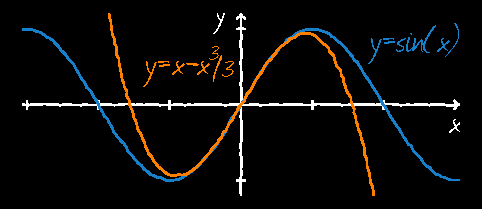
\includegraphics[width=.45\paperwidth]{dlsin}
    \end{center}
\end{textblock}

\begin{textblock}{.4}(.05,.65)
    \begin{center}
        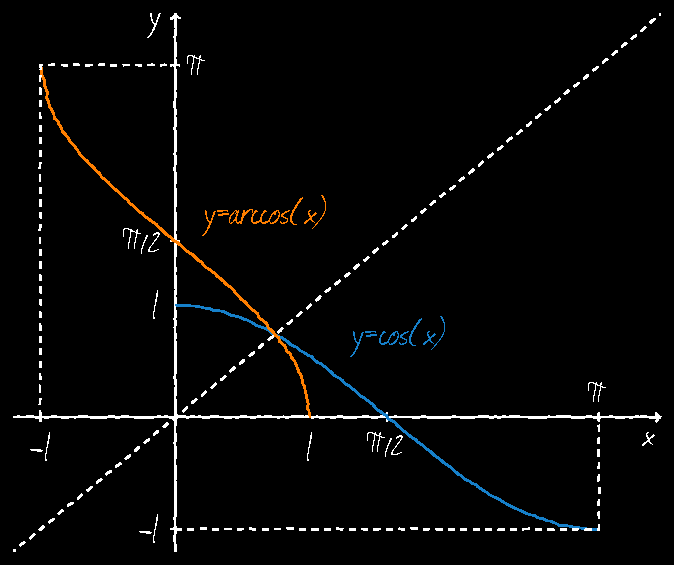
\includegraphics[width=.4\paperwidth]{arccos}
    \end{center}
\end{textblock}


\begin{textblock}{.6}(.05,.6)
    \noindent {\fontsize{20.74}{18}%
    \textcolor{white}{$\displaystyle(a+b)^n = \sum_{k=0}^n 
                \binom{n}{k} a^kb^{n-k}$}}
\end{textblock}


\begin{textblock}{.4}(.4,.77)
    \noindent {\fontsize{17.28}{18}%
    \textcolor{white!80}{$\displaystyle 
                \neg (p\vee q) \equiv (\neg p)\wedge (\neg q)$}}
\end{textblock}

\begin{textblock}{.4}(.1,.93)
    \noindent {\fontsize{14.4}{18}%
    \textcolor{white!50}{$\displaystyle 
                \binom{n}{k} = \frac{n!}{k!(n-k)!}$}}
\end{textblock}


\begin{textblock}{.6}(.5,.69)
    \noindent {\fontsize{17.28}{18}%
    \textcolor{white!10}{$\displaystyle 
                \zeta_k = |a|^{1/n} \mathrm{e}^{i(\mathrm{arg}(a)+2k\pi)/n}$}}
\end{textblock}


\begin{textblock}{.3}(.75,.73)
    \noindent {\fontsize{17.28}{18}%
    \textcolor{white!10}{$\displaystyle \mathrm{e}^{i\pi}+1=0$}}
\end{textblock}



\null\newpage\pagestyle{nexus}

\tableofcontents

\chapter{Histogram Equalization}

\section{OverView}
(a) Write a computer program for computing the histogram of an image.

(b) Implement the histogram equalization technique.

(c) Your program must be general to allow any gray-level image as its input.

As a minimum, your report should include the original image, a plot of its histogram, a plot of the transformation function, the enhanced image, and a plot of its histogram.
\section{Generate the Histogram}
\subsection{Function}
Generating the histogram of an image using following function:\\
\begin{align}
H(i) = the\ number\ of\ pixel\ whose\ value\ euquals\ to\ i
\end{align}
\subsection{Histogram}
The histogram pictures of Fig1.jpg and Fig2.jpg are listed as follows:
\begin{figure}[!htb]
   \centering  
   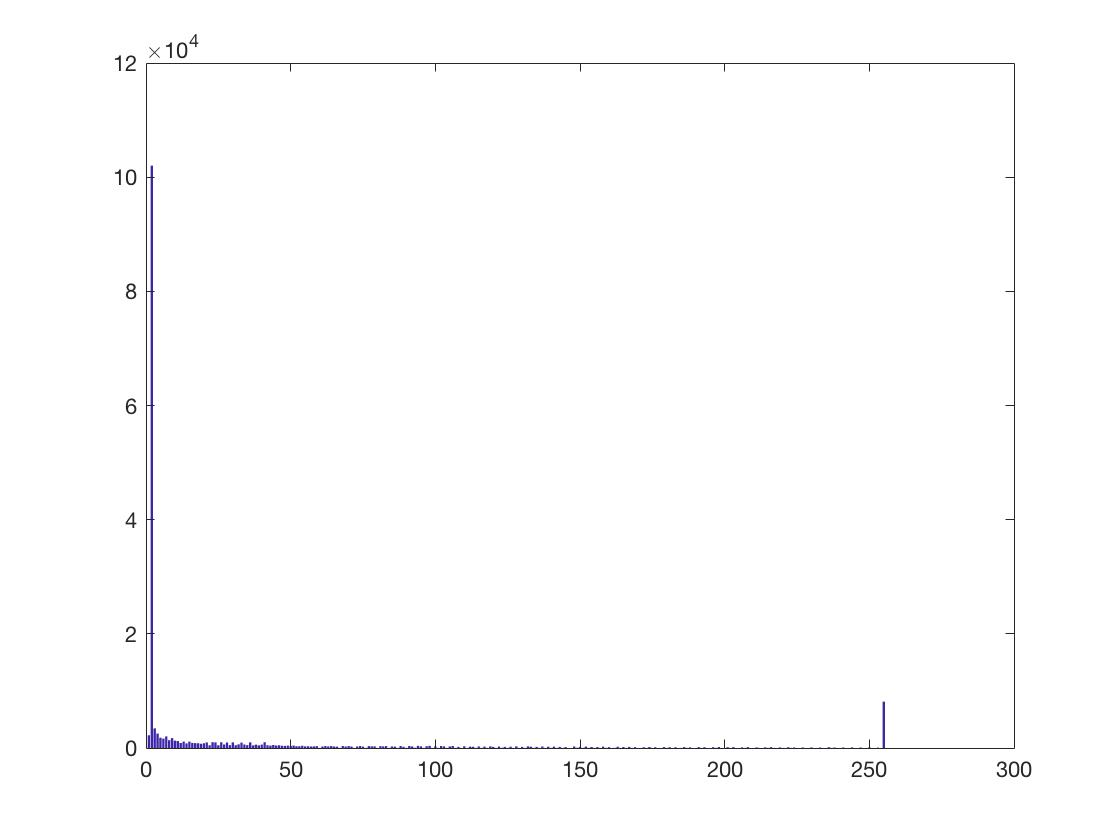
\includegraphics[width=1.0\textwidth]{images/1/histogram1.jpg}
   \caption{Histogram of fig1.jpg}  
\end{figure}
\begin{figure}[!htb]
   \centering  
   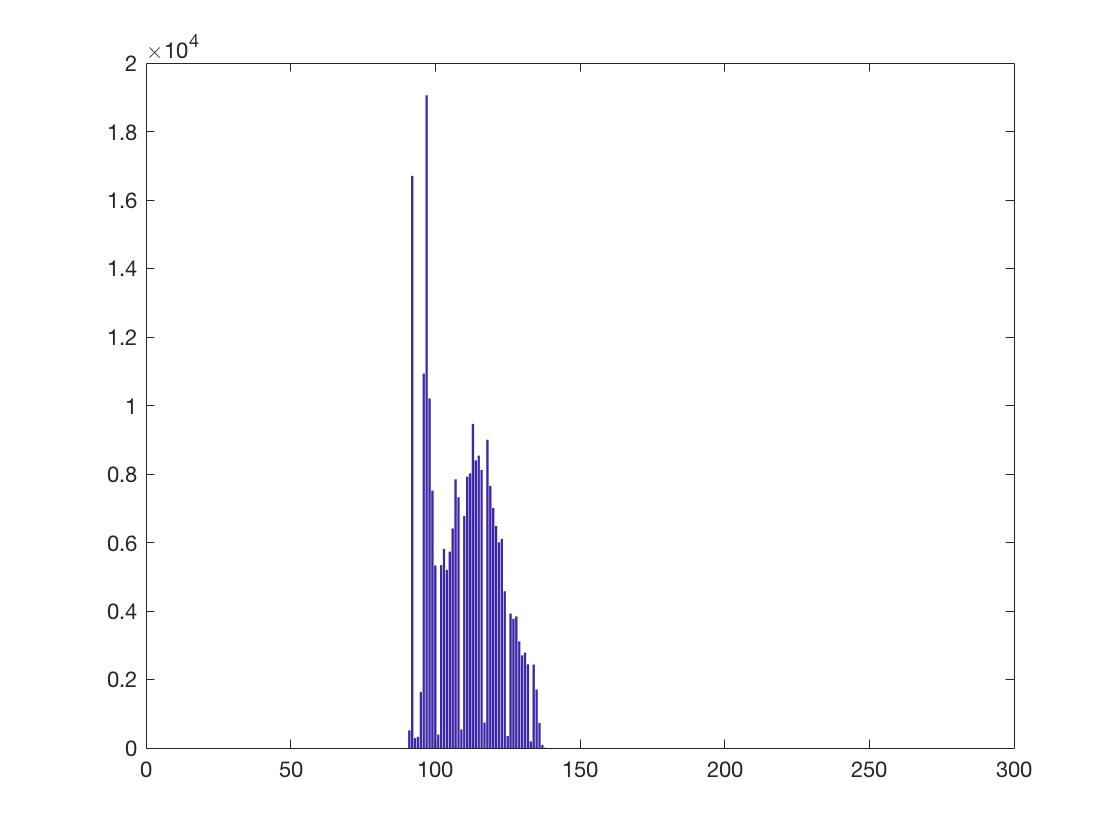
\includegraphics[width=1.0\textwidth]{images/1/histogram2.jpg}
   \caption{Histogram of fig2.jpg}  
\end{figure}

\section{Transfer Function}
\subsection{Implement the Histogram Equalization Technique}
We use those functions to calculate the histogram equalization:\\
\begin{align}
L=Max(image(r,c))\ \forall r \in [1,rows]\ and\ \forall c \in [1,cols]\\
s(r_k) = L*T(r_k) = L*\sum_{j=0}^kP_r(r_j)=L*\sum_{j=0}^k\frac{n_j}{n}
\end{align}
\newpage
\subsection{Transfer Function}
The transfer function of Fig1.jpg and Fig2.jpg are listed as follows:
\begin{figure}[!htb]
   \centering  
   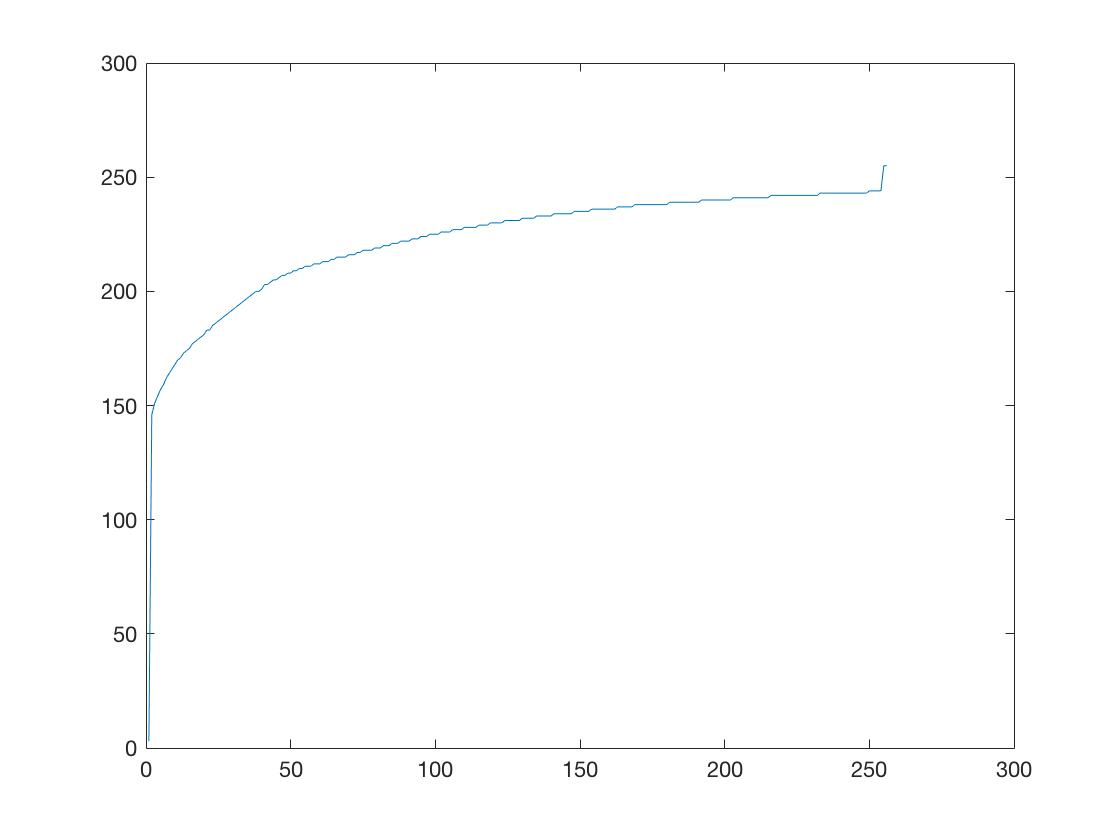
\includegraphics[width=0.8\textwidth]{images/1/transfer_f1.jpg}
   \caption{Transfer Function of fig1.jpg}  
\end{figure}
\begin{figure}[!htb]
   \centering  
   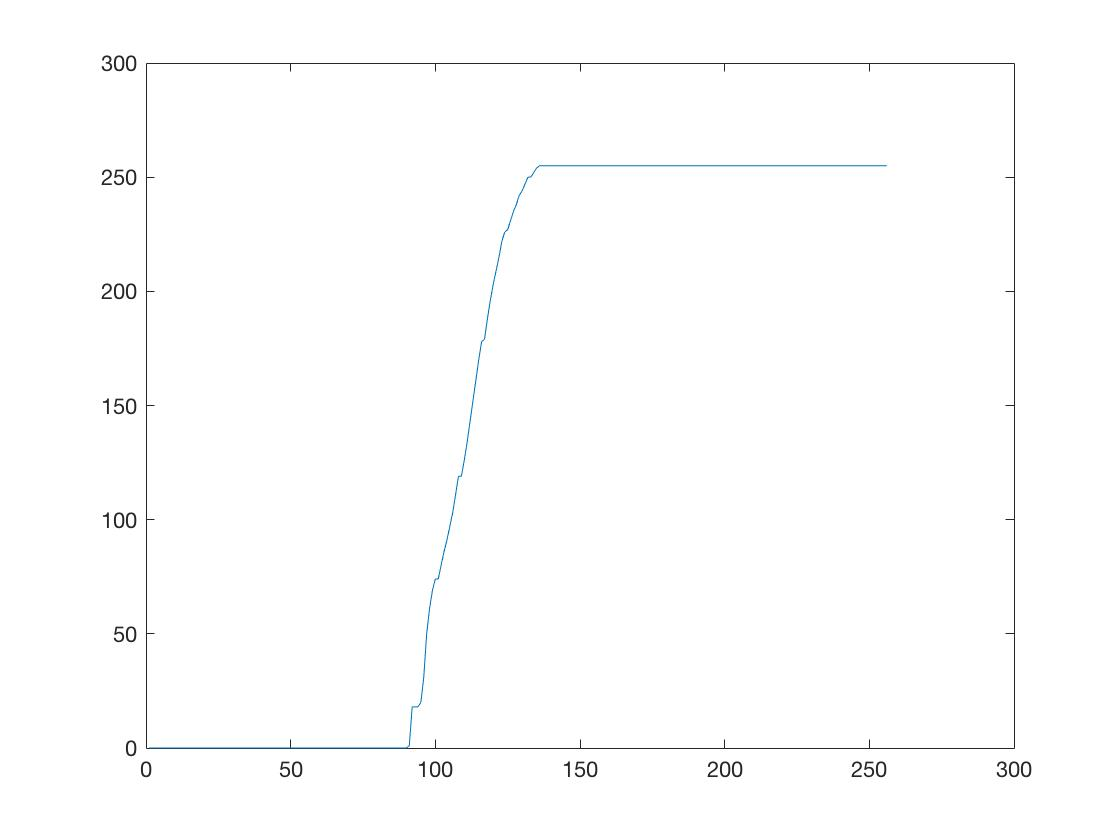
\includegraphics[width=0.8\textwidth]{images/1/transfer_f2.jpg}
   \caption{Transfer Function of fig2.jpg}  
\end{figure}
\section{Enhanced Images}
\subsection{Enhanced Function}
We use the function\\
\begin{align}
New\ Image(r,c) = Transfer\ Function(image(r,c))\ \forall r \in [1,rows]\ and\ \forall c \in [1,cols]
\end{align}
to enhance the original images. 
\subsection{Enhanced Images}
The original images and enhanced images and histogram comparation are listed as follows.
\begin{figure}[!htb]
   \centering  
   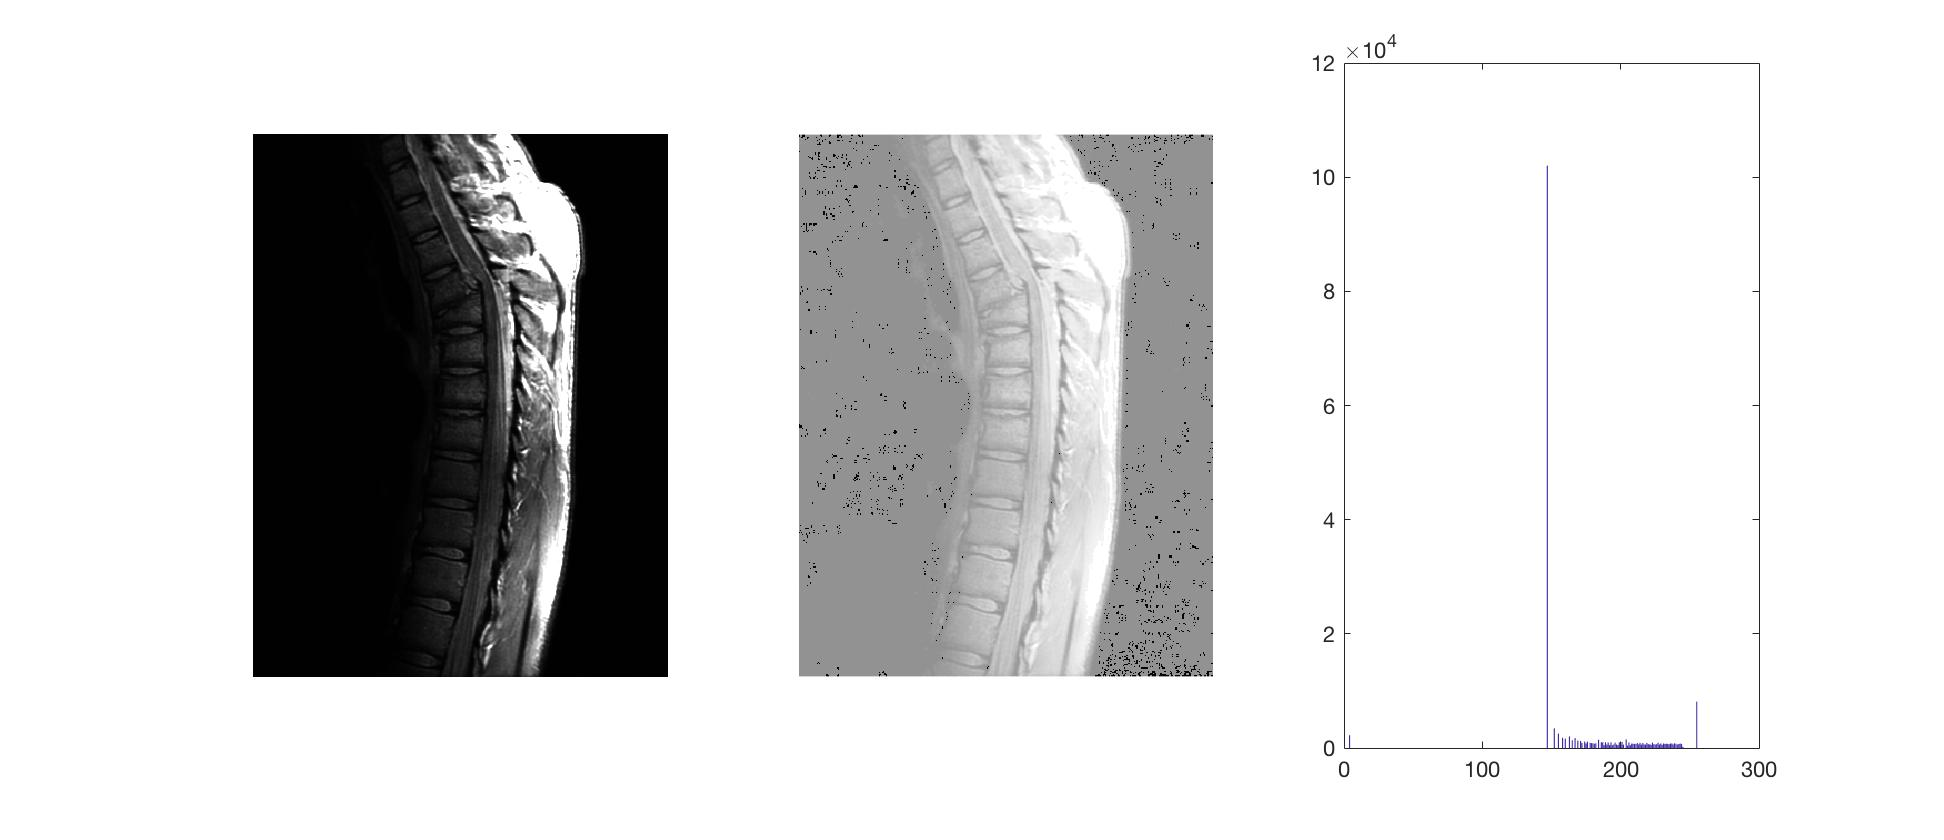
\includegraphics[width=1.0\textwidth]{images/1/image1.jpg}
   \caption{original image and enhanced image and histogram comparation of fig1.jpg}  
\end{figure}
\begin{figure}[!htb]
   \centering  
   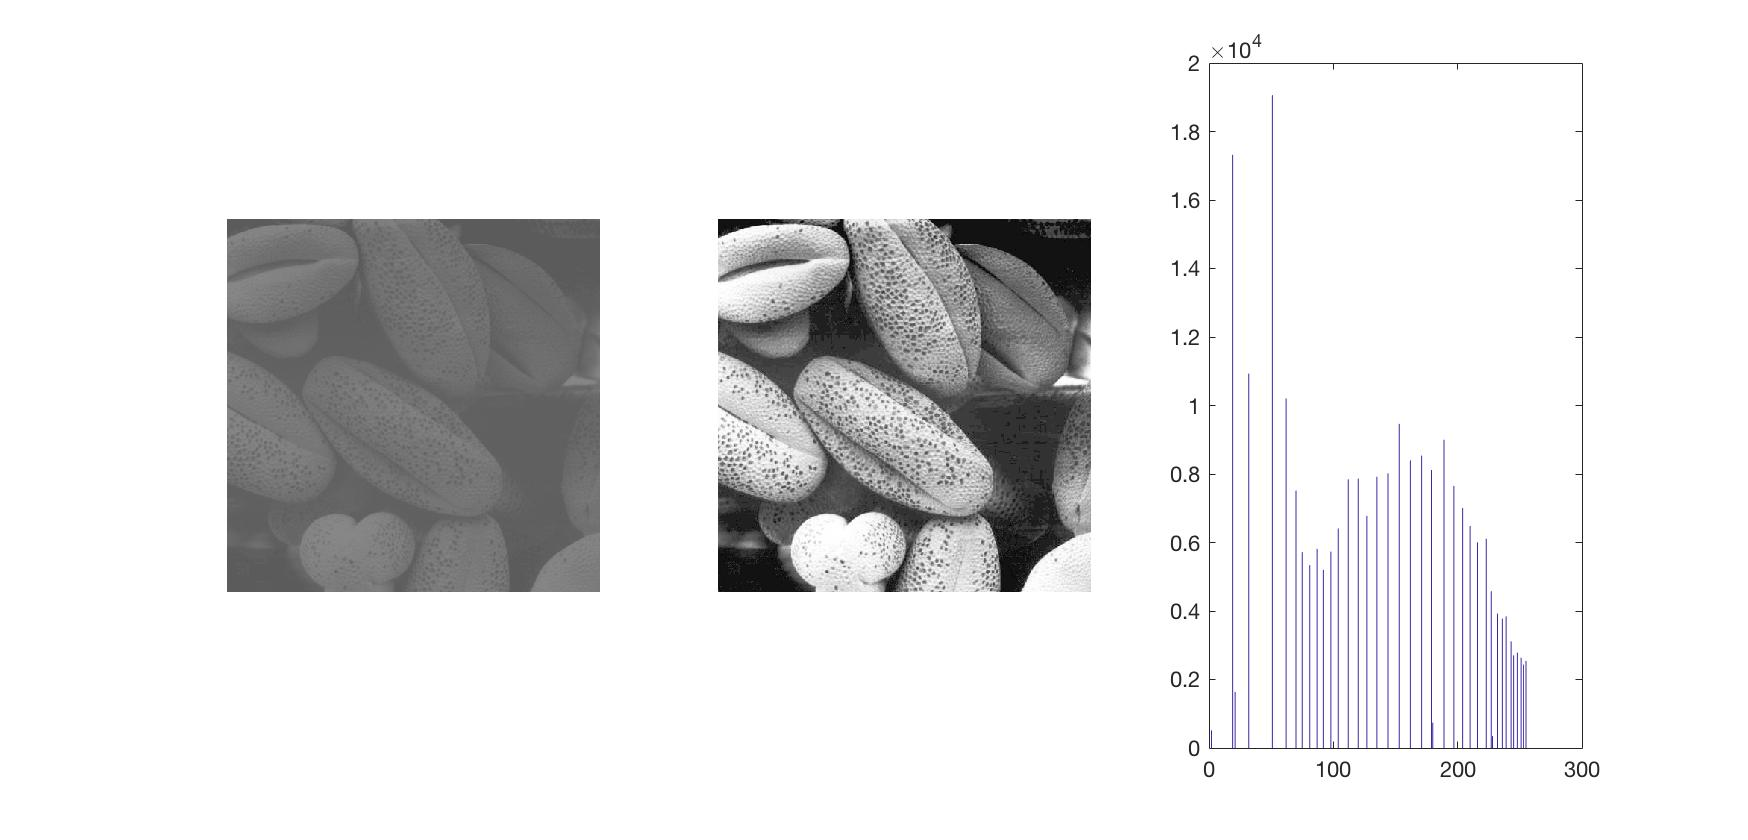
\includegraphics[width=1.0\textwidth]{images/1/image2.jpg}
   \caption{original image and enhanced image and histogram comparation of fig2.jpg}  
\end{figure}





\chapter{Combining spatial enhancement methods}
\section{OverView}
   Implement the image enhancement task of Section 3.7 (Fig 3.43, page 171). The image to be enhanced is skeleton\_orig.tif. You should implement all steps in Figure 3.43. (You are encouraged to implement all functions by yourself, not to directly use Matlab functions such as imfilter or fspecial.)

\section{Image b}
\subsection{Laplacian Transform Filter}
We apply Laplacian Transform on the original image to get the image (b) using the following filter.
\begin{gather*}
\begin{bmatrix} -1&-1&-1 \\ -1&8&-1 \\ -1&-1&-1\end{bmatrix}
\end{gather*}
\subsection{Laplacian Transform}
Image b:
\begin{figure}[!htb]
   \centering  
   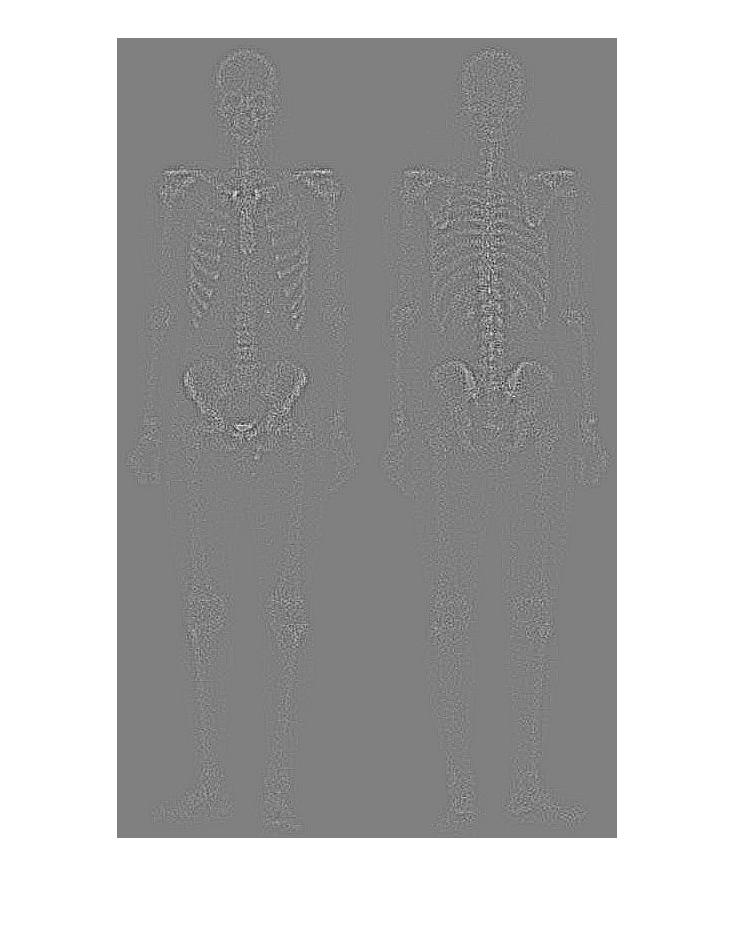
\includegraphics[width=0.625\textwidth]{images/2/b.jpg}
   \caption{Laplacian Transform of skeleton\_orig.tif}  
\end{figure}

\section{Image c}
The we add the Laplacian of the original image to the original image, we will get the new image c. The new image c is a rather noisy sharpened image.\\
Image c:
\begin{figure}[!htb]
   \centering  
   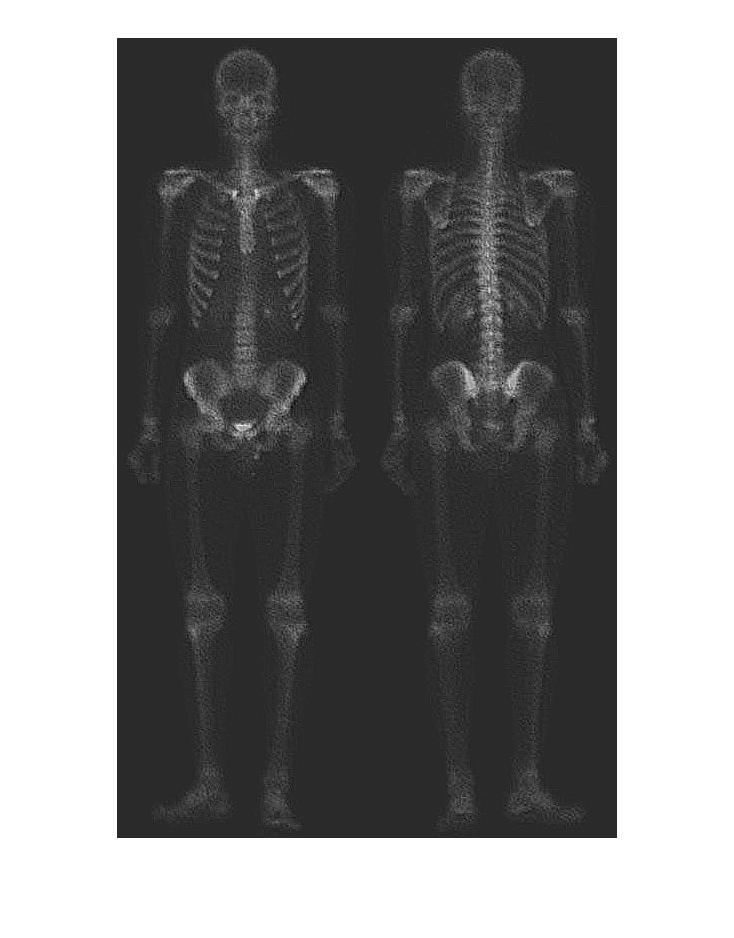
\includegraphics[width=1.0\textwidth]{images/2/c.jpg}
   \caption{Laplacian Transform of skeleton\_orig.tif}  
\end{figure}

\section{Image d}
\subsection{Sobel Gradient Masks}
We will use two mask to separately get the components $g_x$ and $g_y$. Then add the two components together, we will get the the sober gradient of the original image. The new image is as follows. As we can see, edges are much more dominant in this image than in the Laplacian image.\\
$g_x$:
\begin{gather*}
  \begin{bmatrix}
    -1&-2&-1 \\ 0&0&0 \\ 1&2&1
  \end{bmatrix}
\end{gather*}
$g_y$:
\begin{gather*}
  \begin{bmatrix}
    -1&0&1 \\ -2&0&2 \\ -1&0&1
  \end{bmatrix}
\end{gather*}
\subsection{Image d}
Image d:
\begin{figure}[!htb]
   \centering  
   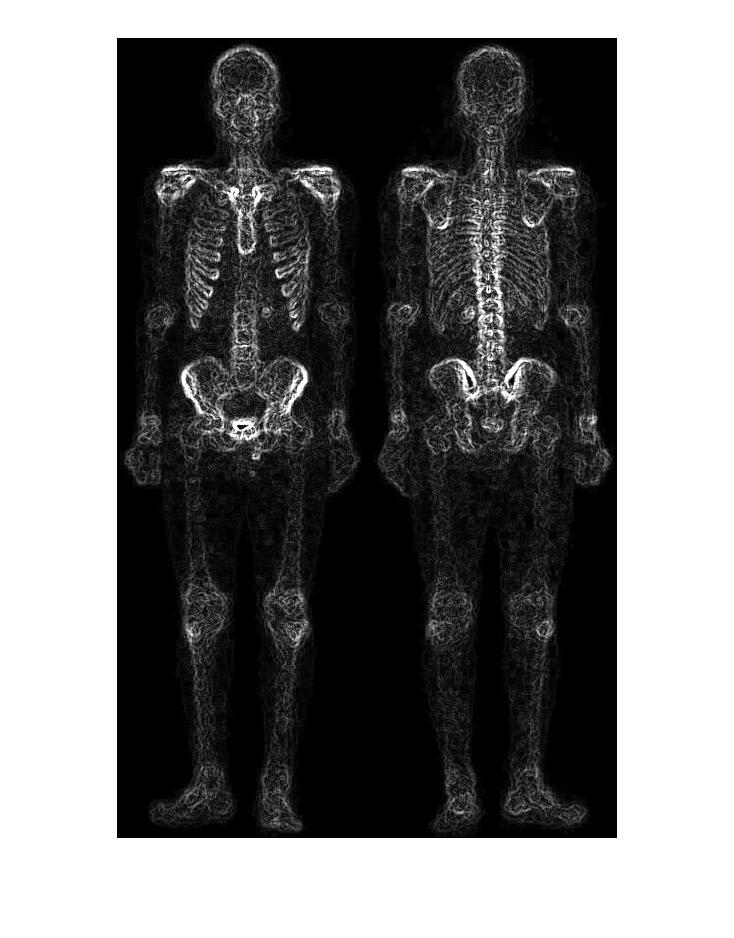
\includegraphics[width=0.625\textwidth]{images/2/d.jpg}
   \caption{Laplacian Transform of skeleton\_orig.tif}  
\end{figure}

\section{Image e}
Image e is formed by smoothing image d by 5*5 mean filter.\\
Image e:
\begin{figure}[!htb]
   \centering  
   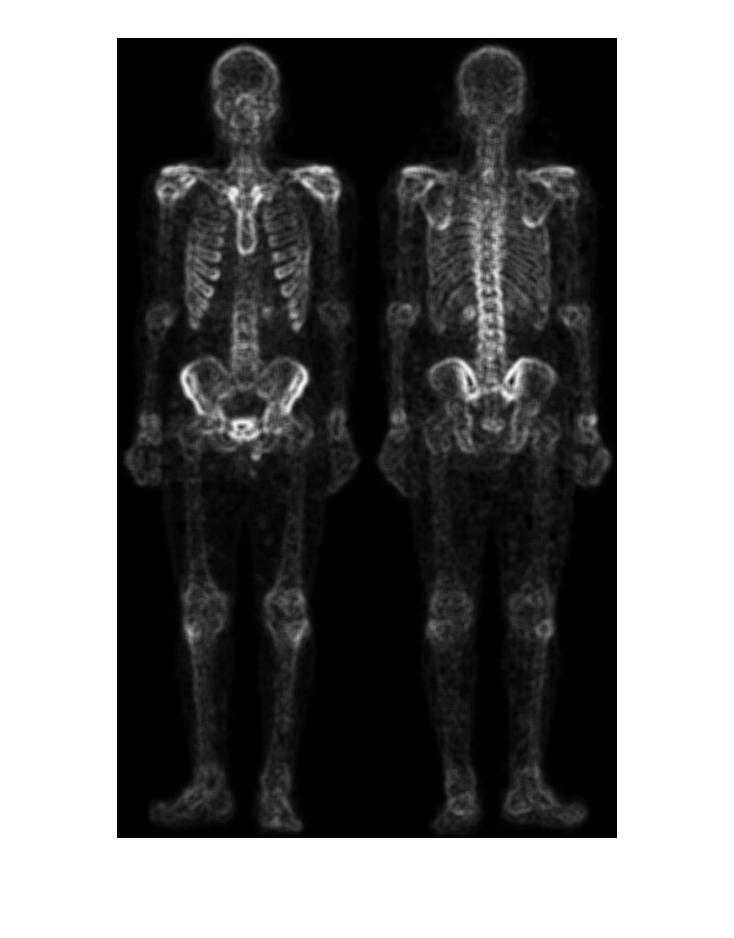
\includegraphics[width=1.0\textwidth]{images/2/e.jpg}
   \caption{Laplacian Transform of skeleton\_orig.tif}  
\end{figure}

\section{Image f}
Image f is formed by the product of Laplacian and smoothed-gradient image.
The dominance of the strong edges and the relative lack of visible noise, which is the key objective behind masking the Laplacian with a smoothed gradient image.\\
Image f:
\begin{figure}[!htb]
   \centering  
   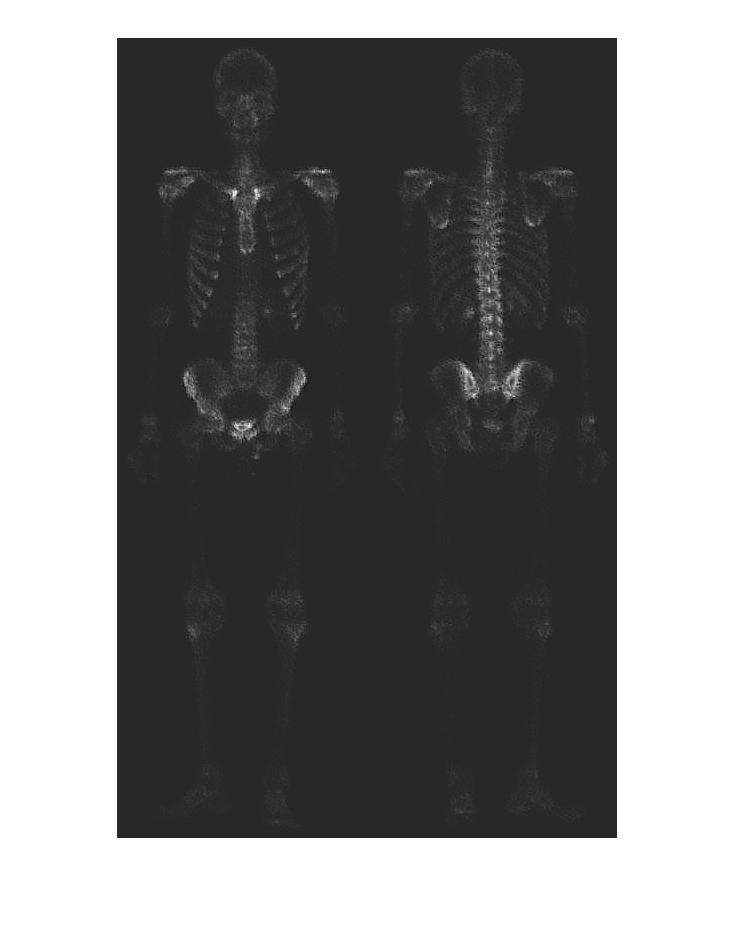
\includegraphics[width=1.0\textwidth]{images/2/f.jpg}
   \caption{Laplacian Transform of skeleton\_orig.tif}  
\end{figure}

\section{Image g}
Adding the image f to the original image and then we get image g.\\
image g:
\begin{figure}[!htb]
   \centering  
   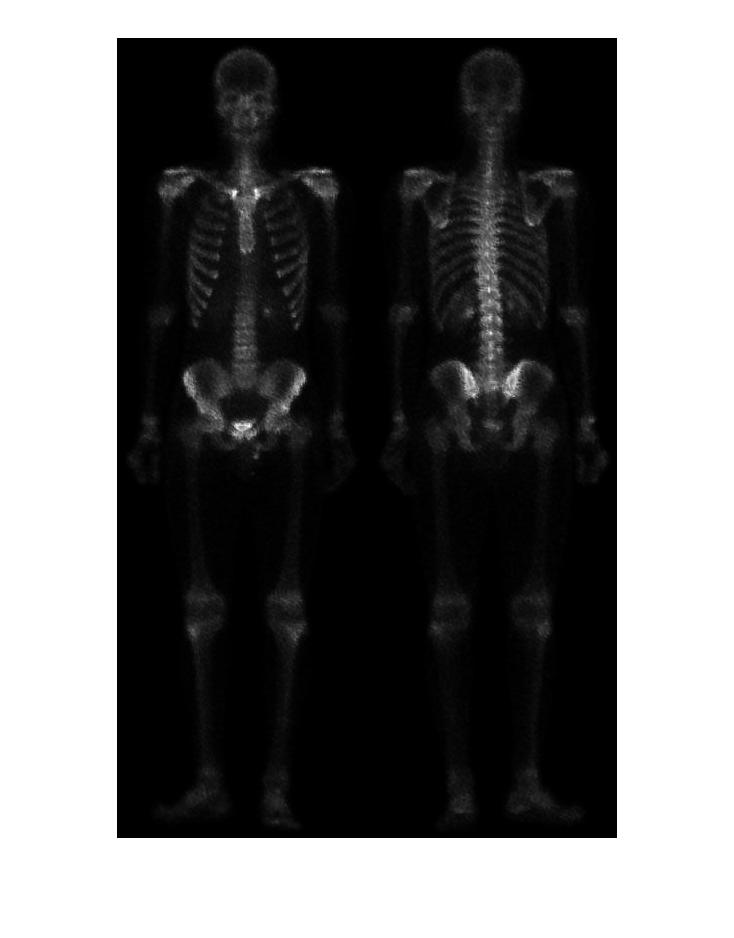
\includegraphics[width=1.0\textwidth]{images/2/g.jpg}
   \caption{Laplacian Transform of skeleton\_orig.tif}  
\end{figure}

\section{Image h}
\subsection{Power-Law Transformation}
We use the following function to perform Power-Law Transformation on image g.
\begin{align}
s=cr^{\gamma}\ (c\ =\ 1\ and\ \gamma \ =\ 1)
\end{align}
\subsection{Image h}
Image h:
\begin{figure}[!htb]
   \centering  
   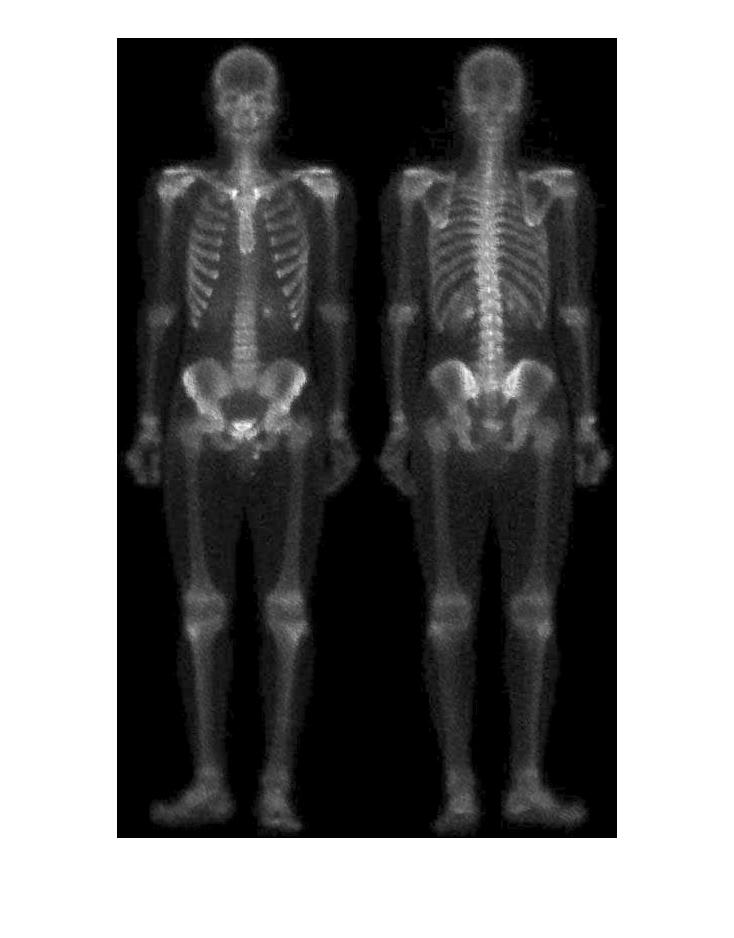
\includegraphics[width=0.85\textwidth]{images/2/h.jpg}
   \caption{Laplacian Transform of skeleton\_orig.tif}  
\end{figure}
\chapter{Filtering in frequency domain}
\section{OverView}
Implement the ideal, Butterworth and Gaussian lowpass and highpass filters and compare the results under different parameters using the image characters\_test\_pattern.tif (this image file can be found at the ftp server ftp://ftp.cs.sjtu.edu.cn:990/lu-ht/DIP/images) as the test pattern.

\section{Fourier Transform}
\subsection{Transform Function}
We first need transform the image to gray image and then use the 2D Fourier transformation belw to change it to the frequence domain.
\begin{align}
F(u,v)=\sum_{x=0}^{M-1}\sum_{y=0}^{N-1}f(x,y)e^{-j2\pi(\frac{ux}{M}+\frac{vy}{N})}\\
f(x,y)=\frac{1}{MN}\sum_{u=0}^{M-1}\sum_{v=0}^{N-1}F(u,v)e^{j2\pi(\frac{ux}{M}+\frac{vy}{N})}
\end{align}
\subsection{Fast Fourier Transform}
The inverse funtion of FFT is as folows:
\begin{align}
F(u+\frac{M}{2},v+\frac{N}{2})&=\sum_{x=0}^{M-1}\sum_{y=0}^{N-1}f(x,y)e^{-j2\pi(\frac{ux+x\frac{M}{2}}{M}+\frac{vy+v\frac{N}{2}}{N})}\\
&=\sum_{x=0}^{M-1}\sum_{y=0}^{N-1}f(x,y)e^{-j2\pi(\frac{ux}{M}+\frac{vy}{N})}*e^{-j\pi x}*e^{-j\pi y}\\
&=\sum_{x=0}^{M-1}\sum_{y=0}^{N-1}-1^{x+y}f(x,y)e^{-j2\pi(\frac{ux}{M}+\frac{vy}{N})}
\end{align}
\section{Filtering}
\begin{itemize}
    \item Expand image$(M*N)$ to image a$((2*M)*(2*N))$
    \item Perform the fourier transform on the new image and get image b
    \item Shift image b and get image c
    \item Perform the convolution on image c and filter and get image d
    \item Shift image d back and get image e
    \item Perform the inverse fourier transform on image e and get image f
    \item Cut image f to get the final result image$(M*N)$;

\end{itemize}
\newpage
\section{Ideal Filter}
\subsection{Ideal Low Pass}
\subsubsection{Ideal Low Pass Filter}
The ideal low pass filter is defined as follows:\\
\begin{eqnarray}H(u,v)=
\begin{cases}
1, &D(u,v)\le0\cr 0, &D(u,v)>0\end{cases}
\end{eqnarray}
\begin{align}
D(u,v)=\sqrt{[(u-\frac{P}{2})^2+(v-\frac{Q}{2})^2]}
\end{align}
\subsubsection{Result}
\begin{figure}[!htb]
   \centering  
   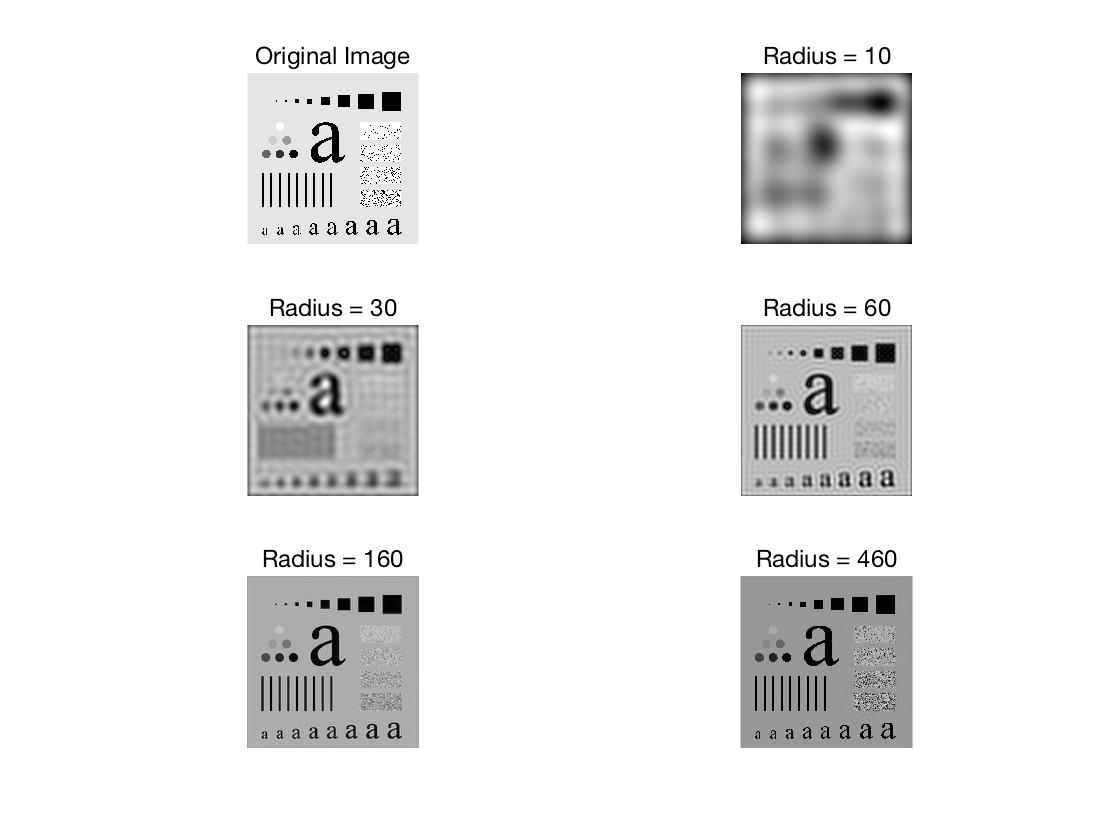
\includegraphics[width=1.0\textwidth]{images/3/ILPF.jpg}
   \caption{ILPF of characters\_test\_pattern.tif}  
\end{figure}

\subsection{Ideal High Pass}
\subsubsection{Ideal High Pass Filter}
The ideal high pass filter is defined as follows:\\
\begin{eqnarray}H(u,v)=
\begin{cases}
0, &D(u,v)\le0\cr 1, &D(u,v)>0\end{cases}
\end{eqnarray}
$D(u,v)$ is defined in $(3.7)$
\subsubsection{Result}
\begin{figure}[!htb]
   \centering  
   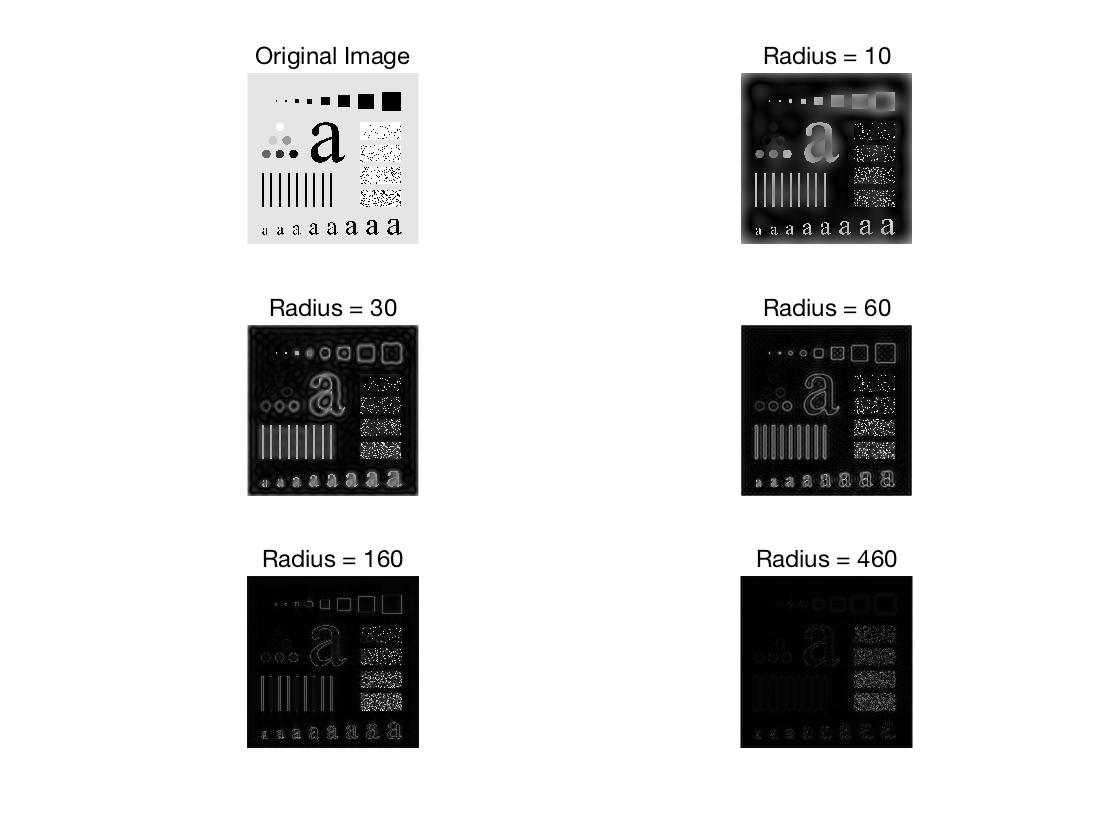
\includegraphics[width=1.0\textwidth]{images/3/IHPF.jpg}
   \caption{ILPF of characters\_test\_pattern.tif}  
\end{figure}
\newpage

\section{Butterworth Filter}
\subsection{Butterworth Low Pass}
\subsubsection{Butterworth Low Pass Filter}
The butterworth low pass filter is defined as follows:\\
\begin{align}
H(u,v)=\frac{1}{1+[D(u,v)/D_0]^{2n}}
\end{align}
$D(u,v)$ is defined in $(3.7)$
\subsubsection{Result}
\begin{figure}[!htb]
   \centering  
   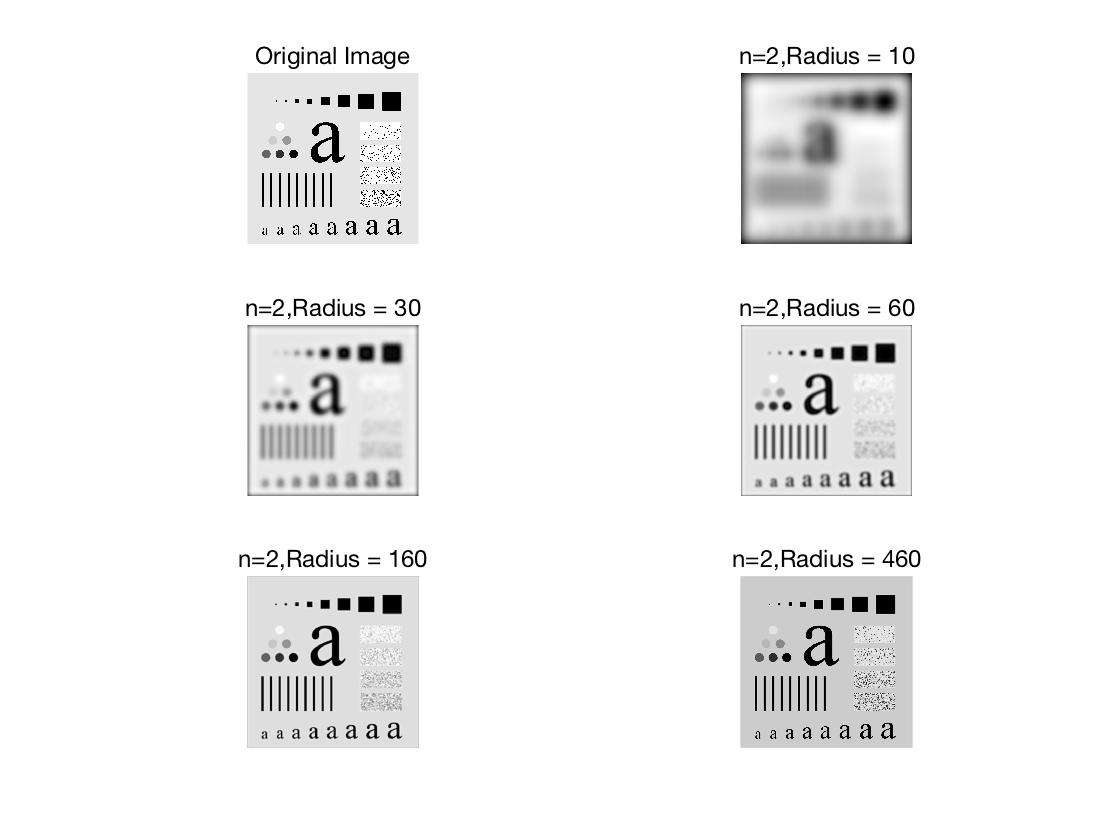
\includegraphics[width=1.0\textwidth]{images/3/BLPF.jpg}
   \caption{BLPF of characters\_test\_pattern.tif}  
\end{figure}

\subsection{Butterworth High Pass}
\subsubsection{Butterworth High Pass Filter}
The butterworth high pass filter is defined as follows:\\
\begin{align}
H(u,v)=\frac{1}{1+[D_0/D(u,v)]^{2n}}
\end{align}
$D(u,v)$ is defined in $(3.7)$
\subsubsection{Result}
\begin{figure}[!htb]
   \centering  
   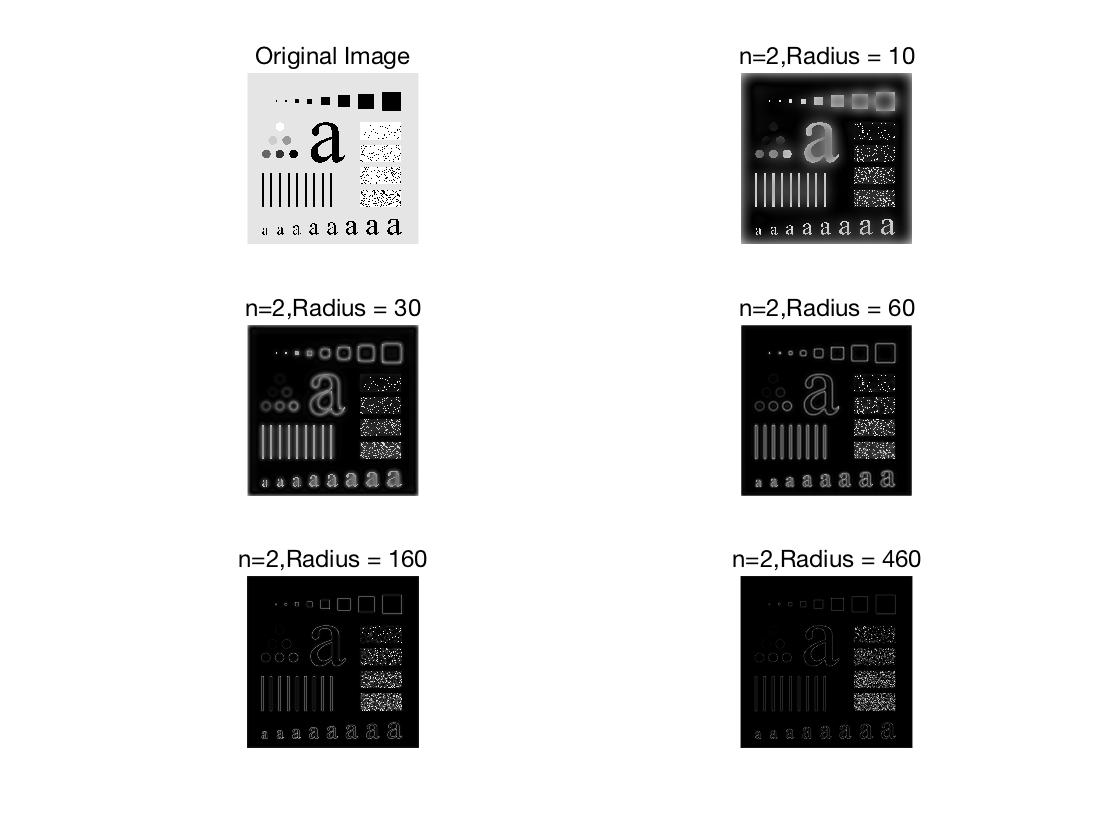
\includegraphics[width=1.0\textwidth]{images/3/BHPF.jpg}
   \caption{BLPF of characters\_test\_pattern.tif}  
\end{figure}
\newpage


\section{Gaussian Filter}
\subsection{Gaussian Low Pass}
\subsubsection{Gaussian Low Pass Filter}
The gaussian low pass filter is defined as follows:\\
\begin{align}
H(u,v)=e^{-\frac{D^2(u,v)}{2\sigma^2}}
\end{align}
$D(u,v)$ is defined in $(3.7)$
\subsubsection{Result}
\begin{figure}[!htb]
   \centering  
   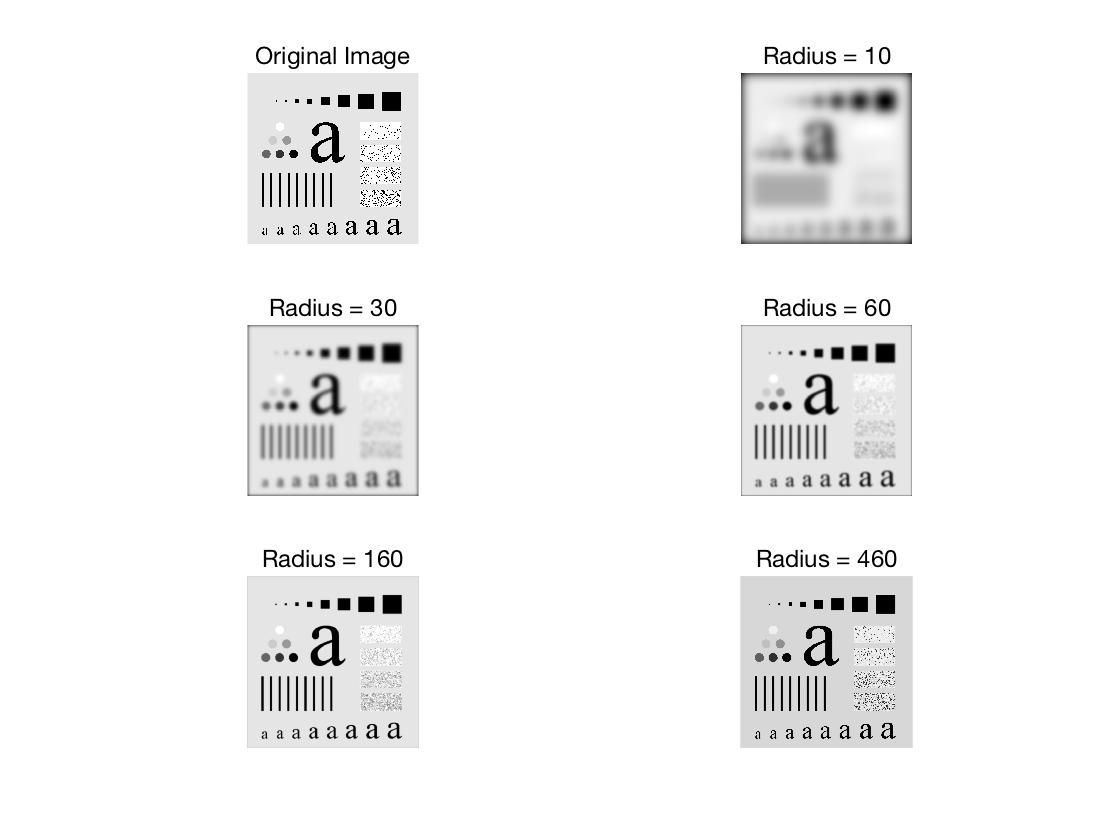
\includegraphics[width=1.0\textwidth]{images/3/GLPF.jpg}
   \caption{GLPF of characters\_test\_pattern.tif}  
\end{figure}

\subsection{Gaussian High Pass}
\subsubsection{Gaussian High Pass Filter}
The gaussian high pass filter is defined as follows:\\
\begin{align}
H(u,v)=1-e^{-\frac{D^2(u,v)}{2\sigma^2}}
\end{align}
$D(u,v)$ is defined in $(3.7)$
\subsubsection{Result}
\begin{figure}[!htb]
   \centering  
   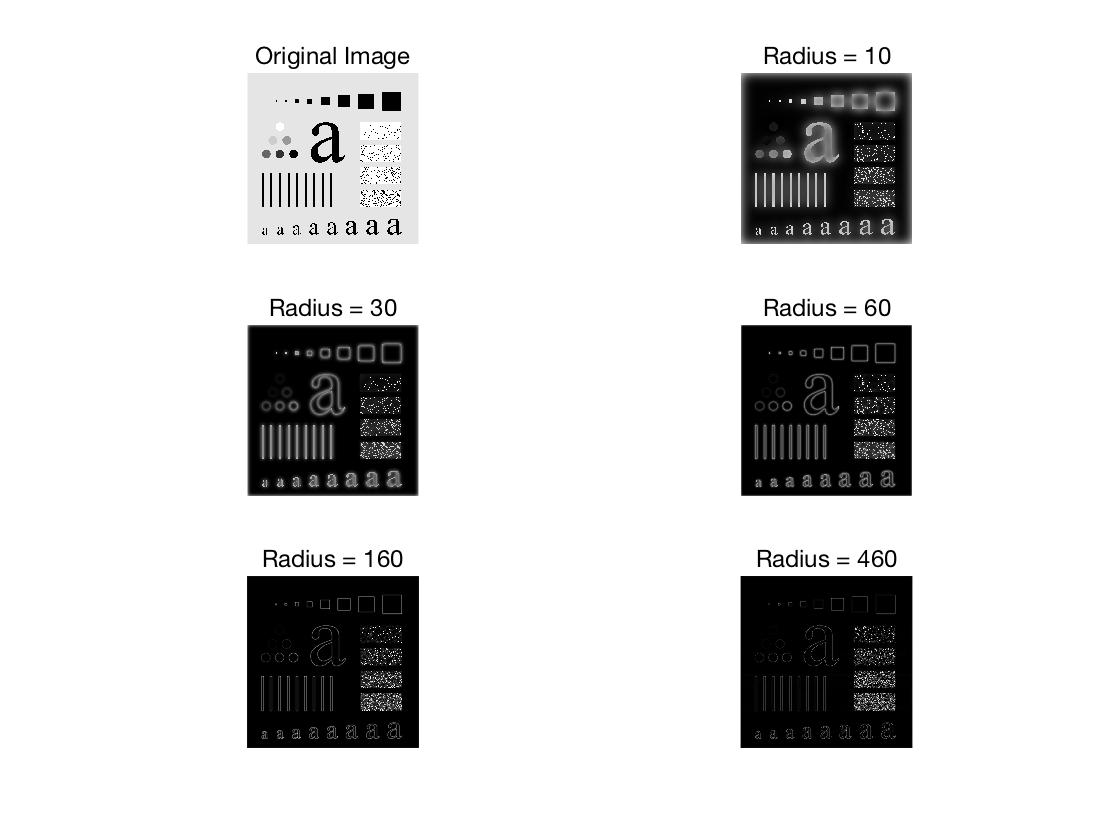
\includegraphics[width=1.0\textwidth]{images/3/GHPF.jpg}
   \caption{GLPF of characters\_test\_pattern.tif}  
\end{figure}




\chapter{Noise and different noise reduction methods}
\section{OverView}
In this problem, you are required to write a program to generate different types of random noise (Uniform, Gaussian, Rayleigh, Gamma, Exponential and Impulse, first started from the uniform noise and then use some functions to convert the uniform noise to Gaussian, Rayleigh, Gamma and Exponential; Impulse noise is generated in a different way, consulting the textbook and some other references) and then add these noises to the test patter image Fig0503(original\_pattern).tif to compare the visual results of the noisy images.

Add some of these noises to the circuit image Circuit.tif (images can be found at ftp://ftp.cs.sjtu.edu.cn:990/lu-ht/DIP/images) and investigate the noise reduction results using different mean filters and order statistics filters as the textbook did at pages 344-352 (Pages 322-329 in the electronic version of the textbook).

\section{Noise}
\subsection{Uniform Noise}
The PDF of $uniform noise$ is given by\\
\begin{eqnarray}p(z)=
\begin{cases}
\frac{1}{b-a}, &if\ a \le z\le b\cr 0, &otherwise\end{cases}
\end{eqnarray}
The mean of this density function is given by\\
\begin{align}
\overline z =\frac{a+b}{2}
\end{align}
and its variance by\\
\begin{align}
\sigma ^{2} = \frac{(b-a)^2}{12}
\end{align}

\begin{figure}[!htb]
   \centering  
   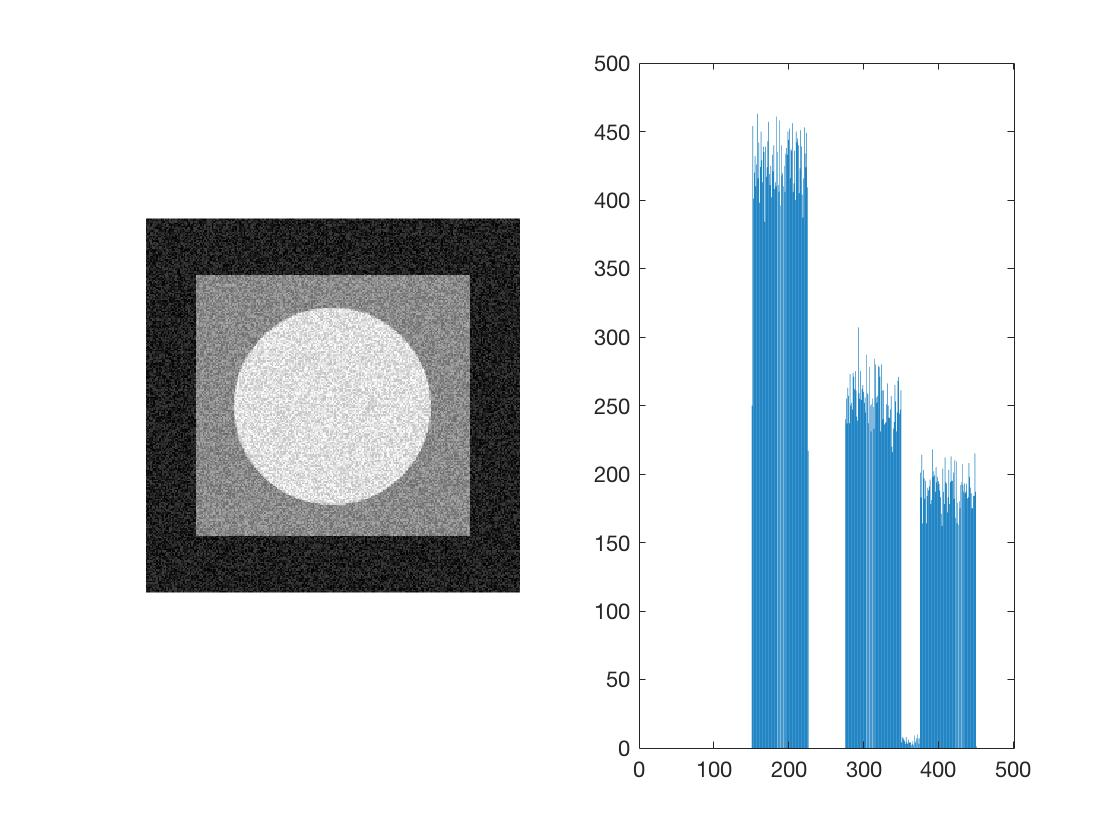
\includegraphics[width=0.5\textwidth]{images/4/uniform.jpg}
   \caption{Uniform Noise}  
\end{figure}
\newpage
\subsection{Gaussian Noise}
The PDF of a $Gaussian$ random variable, z, is given by\\
\begin{align}
p(z) = \frac{1}{\sqrt{2\pi}\sigma}e^{-\frac{(z-\overline z)^2}{z\sigma ^2}}
\end{align}
and it can generate form uniform noise by\\
\begin{align}
X = \sqrt{-2lnU}cos(2\pi V)\\
Y = \sqrt{-2lnU}sin(2\pi V)
\end{align}
$U$ and $V$ come form uniform(0,1).
\begin{figure}[!htb]
   \centering  
   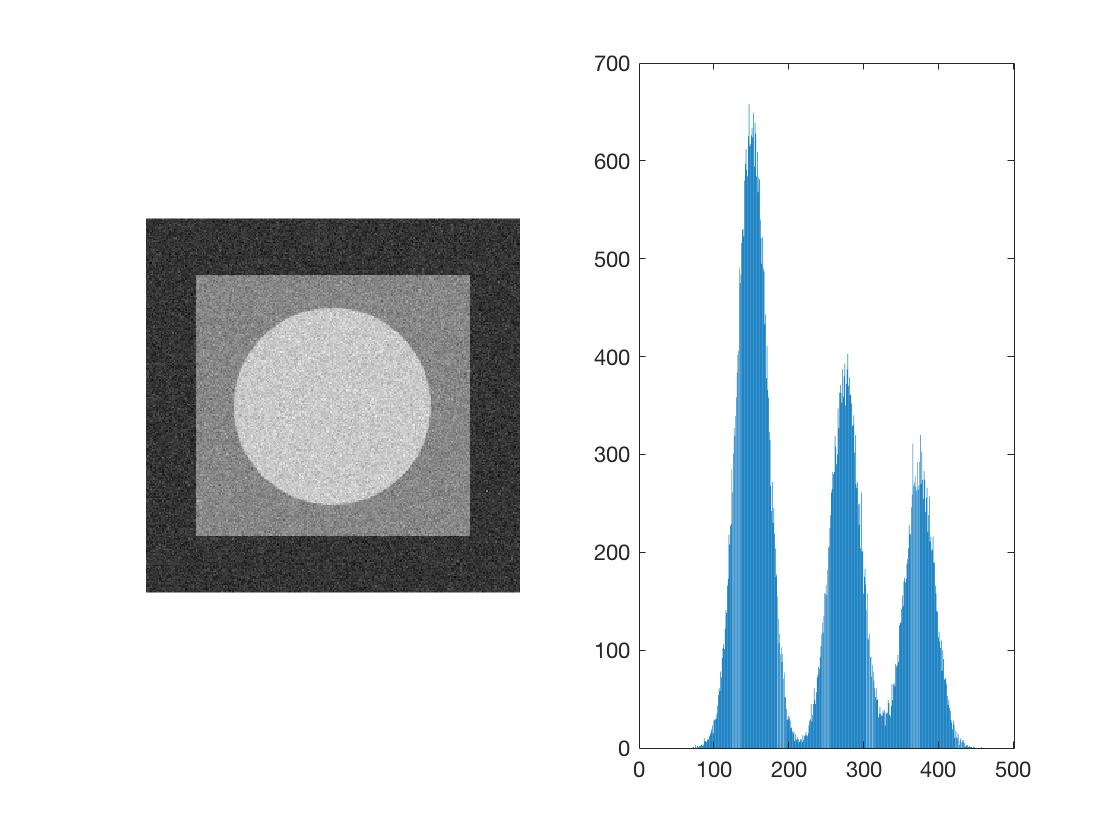
\includegraphics[width=1.0\textwidth]{images/4/gaussian.jpg}
   \caption{Gaussian Noise}  
\end{figure}
\newpage
\subsection{Rayleigh Noise}
The PDF of $Rayleigh noise$ is given by\\
\begin{eqnarray}p(z)=
\begin{cases}
\frac{2}{b}(z-a)e^{-\frac{(z-a)^2}{b}}, &for\ z \ge a\cr 0, &for\ z <a\end{cases}
\end{eqnarray}
The mean and variance of this density are given by\\
\begin{align}
\overline z = a + \sqrt{\frac{b\pi}{4}}
\end{align}
and
\begin{align}
\sigma ^2 = \frac{b(4-\pi)}{4}
\end{align}
and it can generate form uniform noise by\\
\begin{align}
  z=a+\sqrt{-bln[1-U(0,1)]}
\end{align}
\begin{figure}[!htb]
   \centering  
   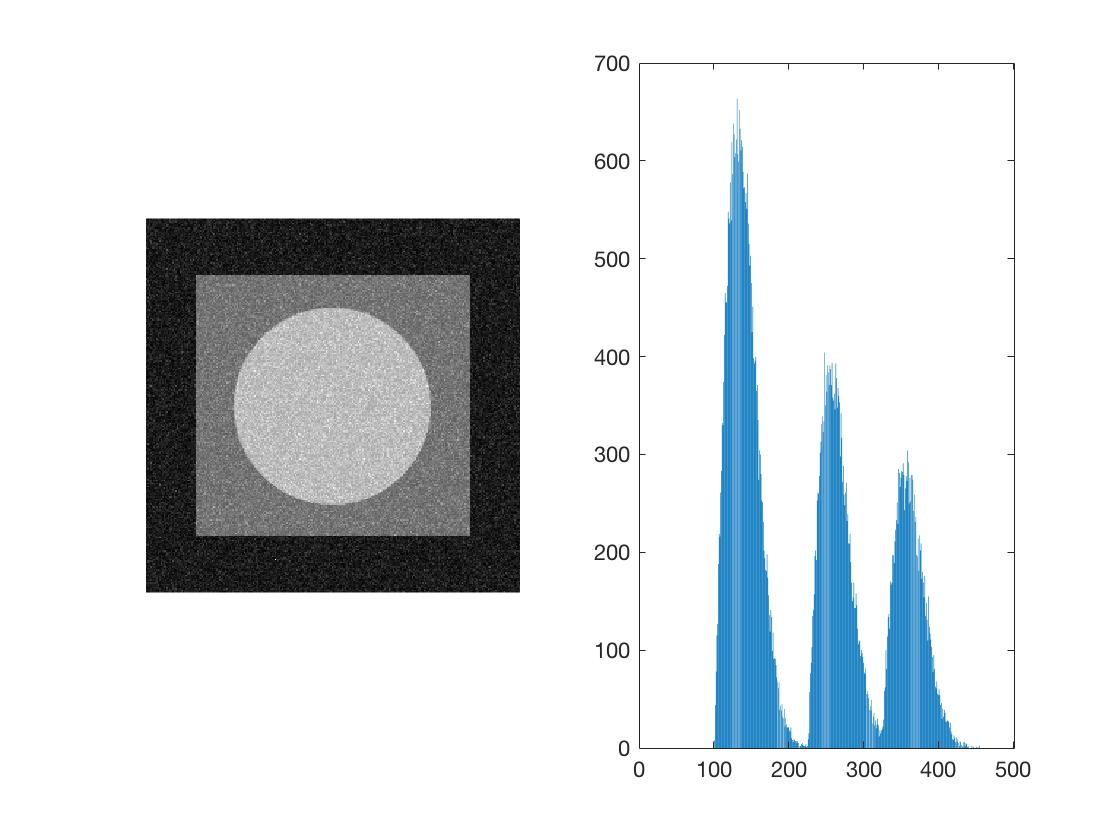
\includegraphics[width=1.0\textwidth]{images/4/rayleigh.jpg}
   \caption{Rayleigh Noise}  
\end{figure}
\newpage
\subsection{Erlang(Gamma) Noise}
The PDF of $Erlang noise$ is given by\\
\begin{eqnarray}p(z)=
\begin{cases}
\frac{a^bz^{b-1}}{(b-1)!}e^{-az}, &for\ z \ge 0\cr 0, &for\ z <0\end{cases}
\end{eqnarray}
The mean and variance of this density are given by\\
\begin{align}
\overline z = \frac{b}{a}
\end{align}
and\\
\begin{align}
 \sigma ^2 = \frac{b}{a^2}
\end{align}
and it can generate form uniform noise by\\
\begin{align}
  E_i = -\frac{1}{a}ln[1-U(0,1)]\\
  z=E_1+E_2+\cdots+E_b
\end{align}
\begin{figure}[!htb]
   \centering  
   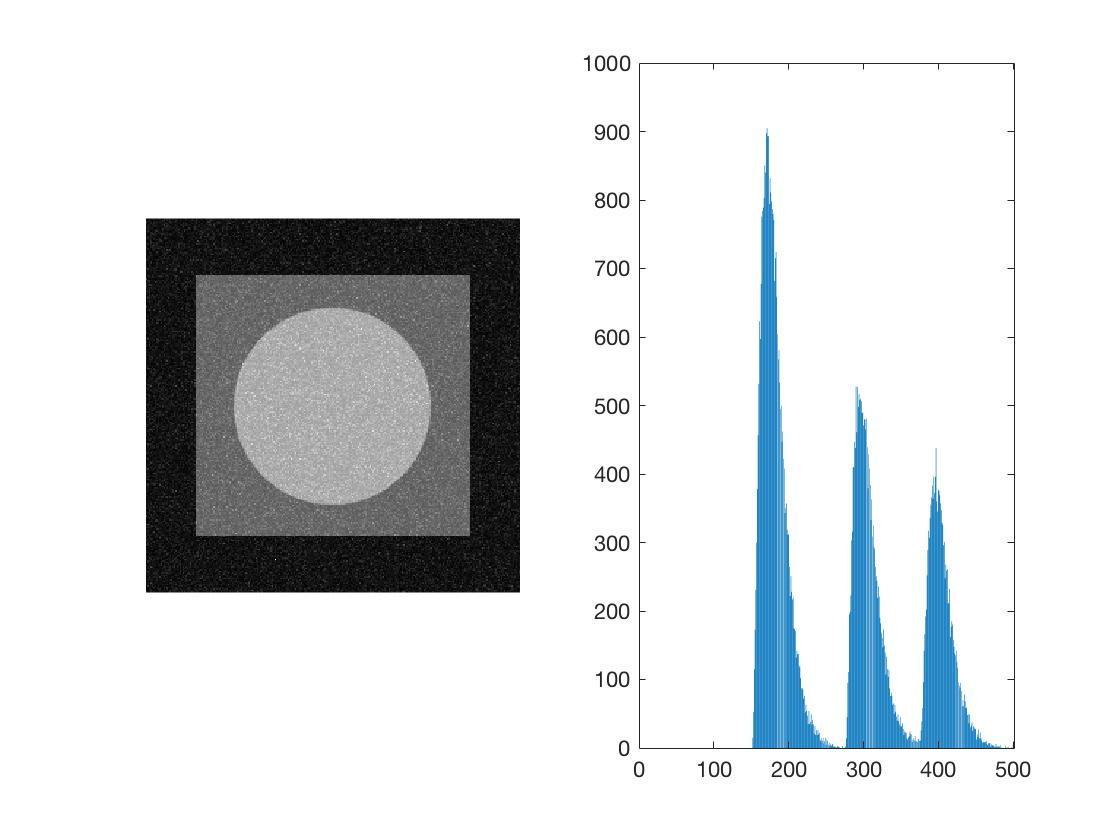
\includegraphics[width=0.9\textwidth]{images/4/gamma.jpg}
   \caption{Gamma Noise}  
\end{figure}
\newpage
\subsection{Exponential Noise}
The PDF of $exponential noise$ is given by\\
\begin{eqnarray}p(z)=
\begin{cases}
ae^{-az}, &for\ z \ge 0\cr 0, &for\ z <0\end{cases}
\end{eqnarray}
The mean and variance of this density function are\\
\begin{align}
\overline z = \frac{1}{a}
\end{align}
and\\
\begin{align}
\sigma ^2 = \frac{1}{a^2}
\end{align}
and it can generate form uniform noise by\\
\begin{align}
z = -\frac{1}{a}ln[1-U(0,1)]
\end{align}
\begin{figure}[!htb]
   \centering  
   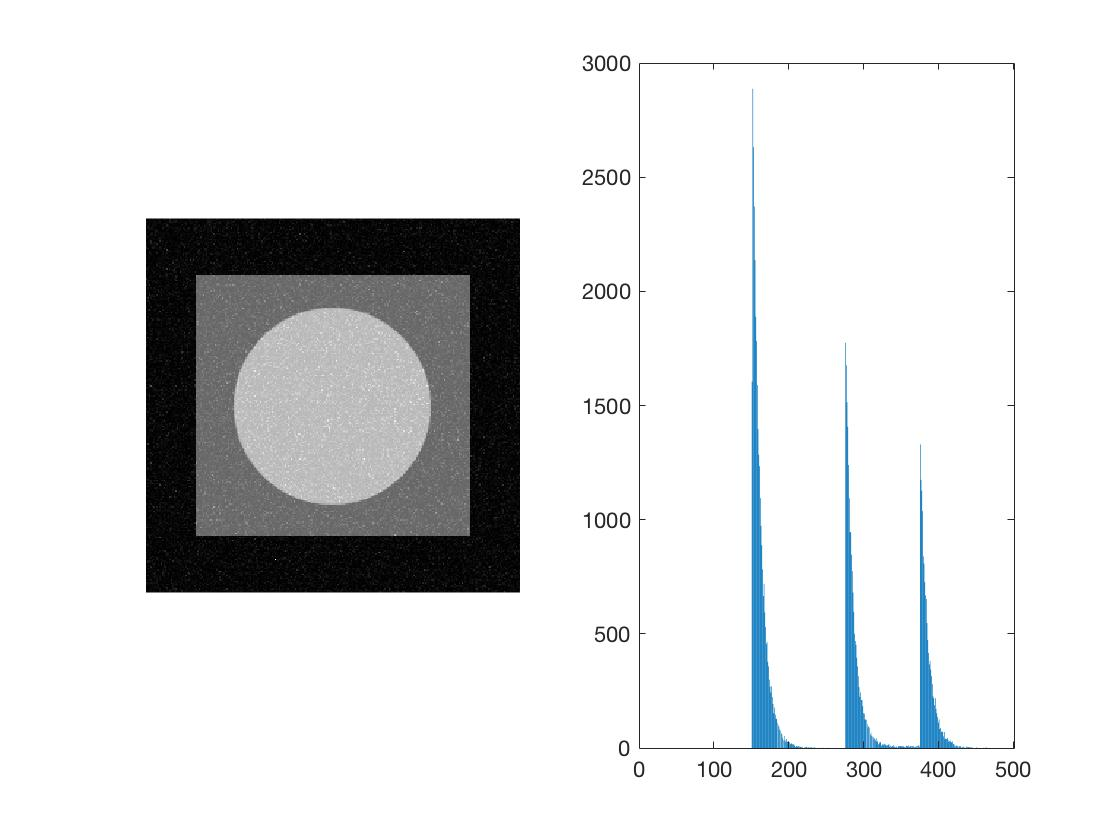
\includegraphics[width=0.9\textwidth]{images/4/exponential.jpg}
   \caption{Exponential Noise}
\end{figure}
\newpage
\subsection{Impulse Noise}
The PDF of $(bipolar) impulse noise$ is given by\\
\begin{eqnarray}p(z)=
\begin{cases}
P_a, &for\ z=a \cr P_b, &for\ z = b\cr 0,&otherwise\end{cases}
\end{eqnarray}
\begin{figure}[!htb]
   \centering  
   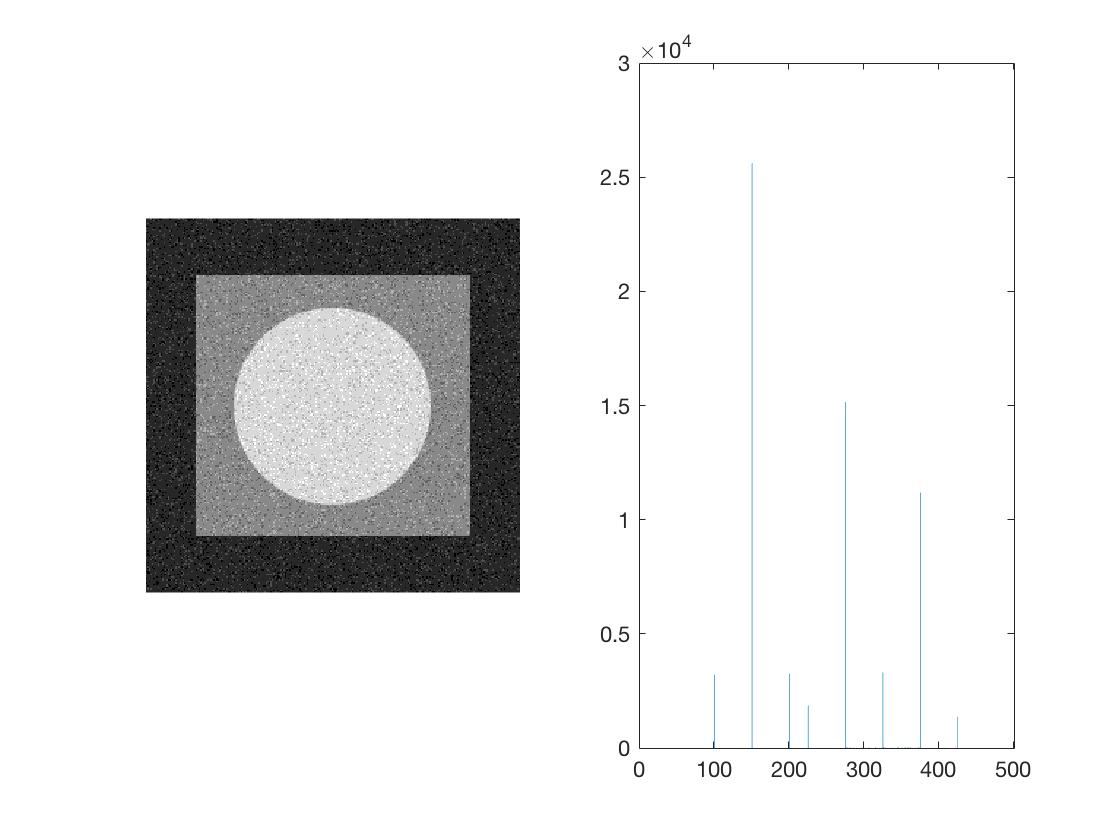
\includegraphics[width=1.0\textwidth]{images/4/impulse.jpg}
   \caption{Impulse Noise}
\end{figure}
\newpage

\section{Mean Filters}
\subsection{Filters}
\subsubsection{Arithmetic mean filter}
\begin{align}
\hat{f}(x,y)=\frac{1}{mn}\sum_{(s,t)\in S_{xy}}g(s,t)
\end{align}
\subsubsection{Geometric mean filter}
\begin{align}
\hat{f}(x,y)=[\prod_{(s,t)\in S_{xy}}g(s,t)]^{\frac{1}{mn}}
\end{align}
\subsubsection{Harmonic mean filter}
\begin{align}
\hat{f}(x,y) = \frac{mn}{\sum_{(s,t)\in S_{xy}}\frac{1}{g(s,t)}}
\end{align}
\subsubsection{Contraharmonic mean filter}
\begin{align}
\hat{f}(x,y) = \frac{\sum_{(s,t)\in S_{xy}}g(s,t)^{Q+1}}{\sum_{(s,t)\in S_{xy}}g(s,t)^Q}
\end{align}
\subsection{Results}
\begin{figure}[!htb]
   \centering  
   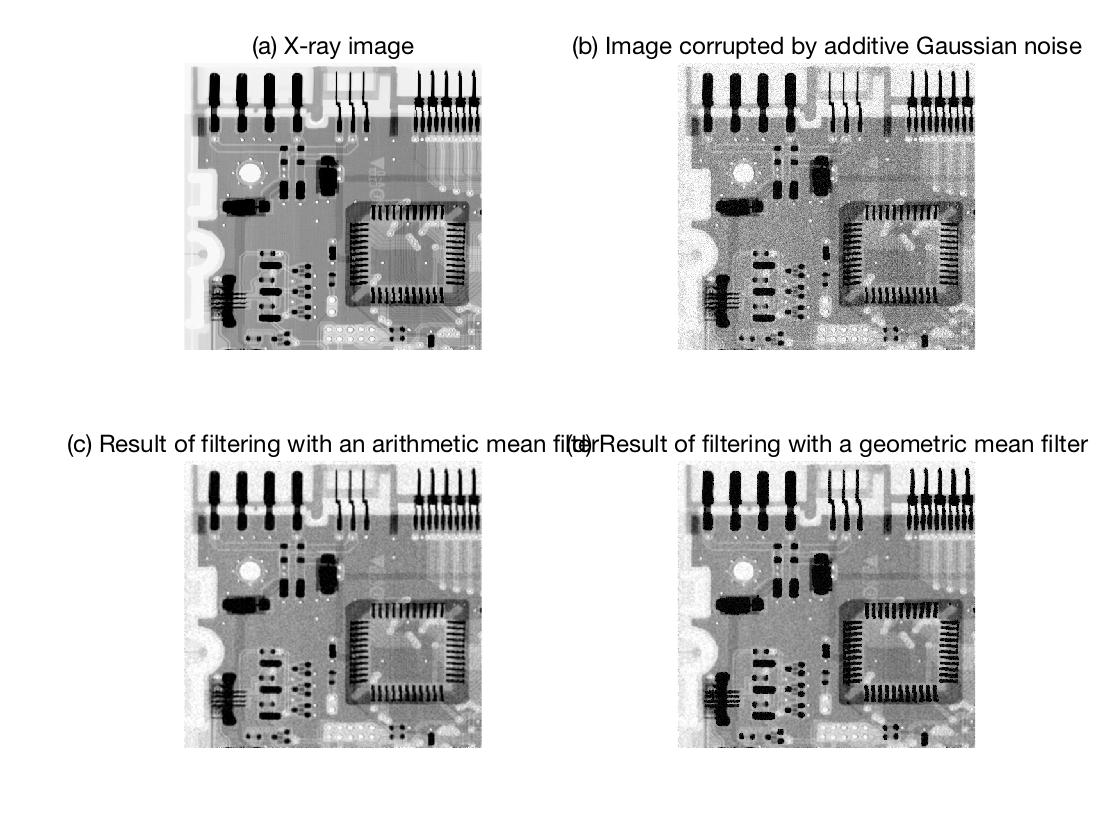
\includegraphics[width=0.75\textwidth]{images/4/mean1.jpg}
   \caption{Original Book FIGURE 5.7}
\end{figure}
\newpage
\begin{figure}[!htb]
   \centering  
   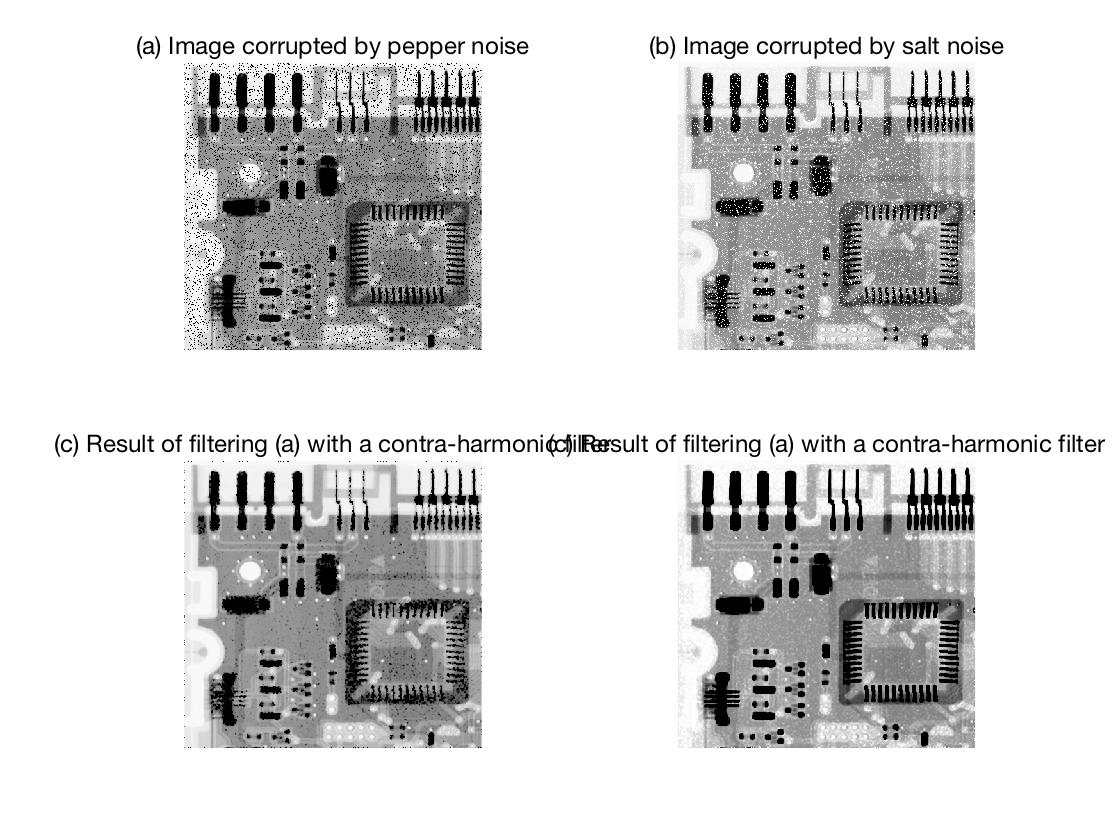
\includegraphics[width=1.0\textwidth]{images/4/mean2.jpg}
   \caption{Original Book FIGURE 5.8}
\end{figure}
\begin{figure}[!htb]
   \centering  
   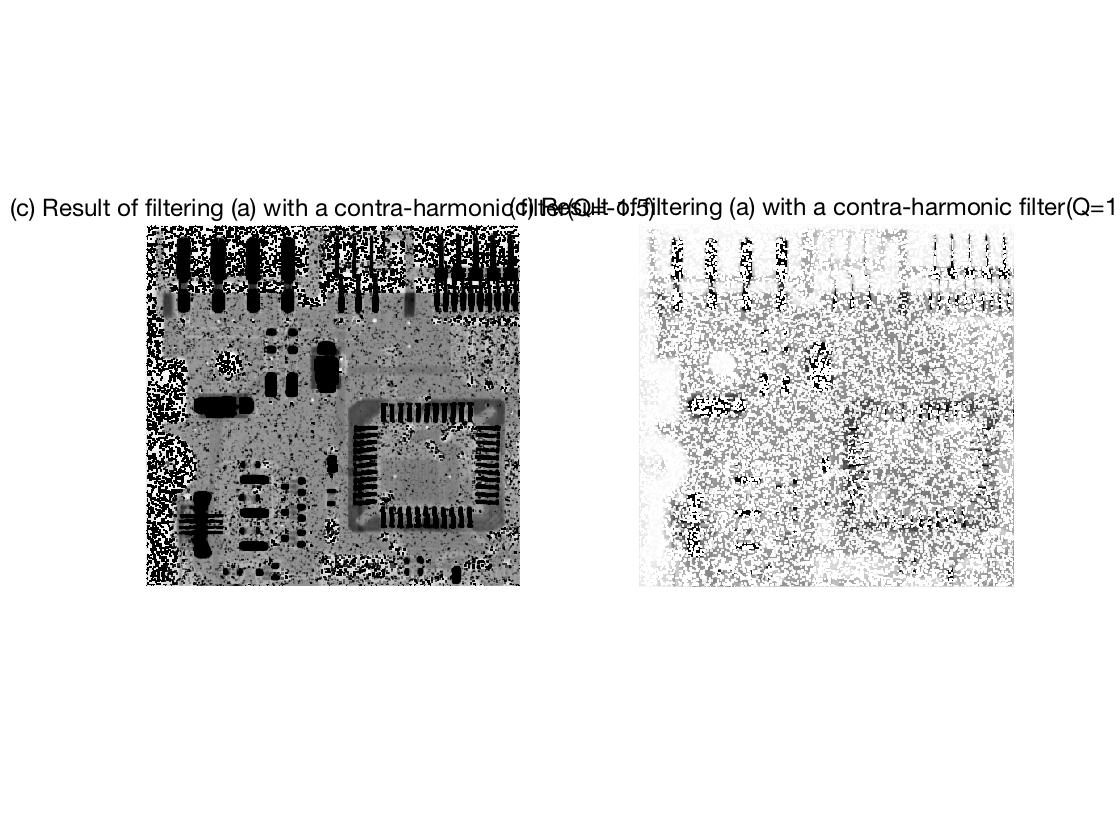
\includegraphics[width=0.7\textwidth]{images/4/mean3.jpg}
   \caption{Original Book FIGURE 5.9}
\end{figure}
\newpage

\section{Order-Statistic Filters}
\subsection{Filters}
\subsubsection{Median filter}
\begin{align}
\hat{f}(x,y) = {median}_{(s,t)\in S_{xy}}{g(s,t)}
\end{align}
\subsubsection{Max filters}
\begin{align}
\hat{f}(x,y) = {max}_{(s,t)\in S_{xy}}{g(s,t)}
\end{align}
\subsubsection{Min filters}
\begin{align}
\hat{f}(x,y) = {min}_{(s,t)\in S_{xy}}{g(s,t)}
\end{align}
\subsubsection{Midpoint filter}
\begin{align}
\hat{f}(x,y) = \frac{1}{2}[{max}_{(s,t)\in S_{xy}}{g(s,t)}+{min}_{(s,t)\in S_{xy}}{g(s,t)}]
\end{align}
\subsubsection{Alpha-trimmed mean filter}
\begin{align}
\hat{f}(x,y) = \frac{1}{mn-d}\sum_{(s,t)\in S_{xy}}g_r(s,t)
\end{align}
\newpage
\subsection{Results}
\begin{figure}[!htb]
   \centering  
   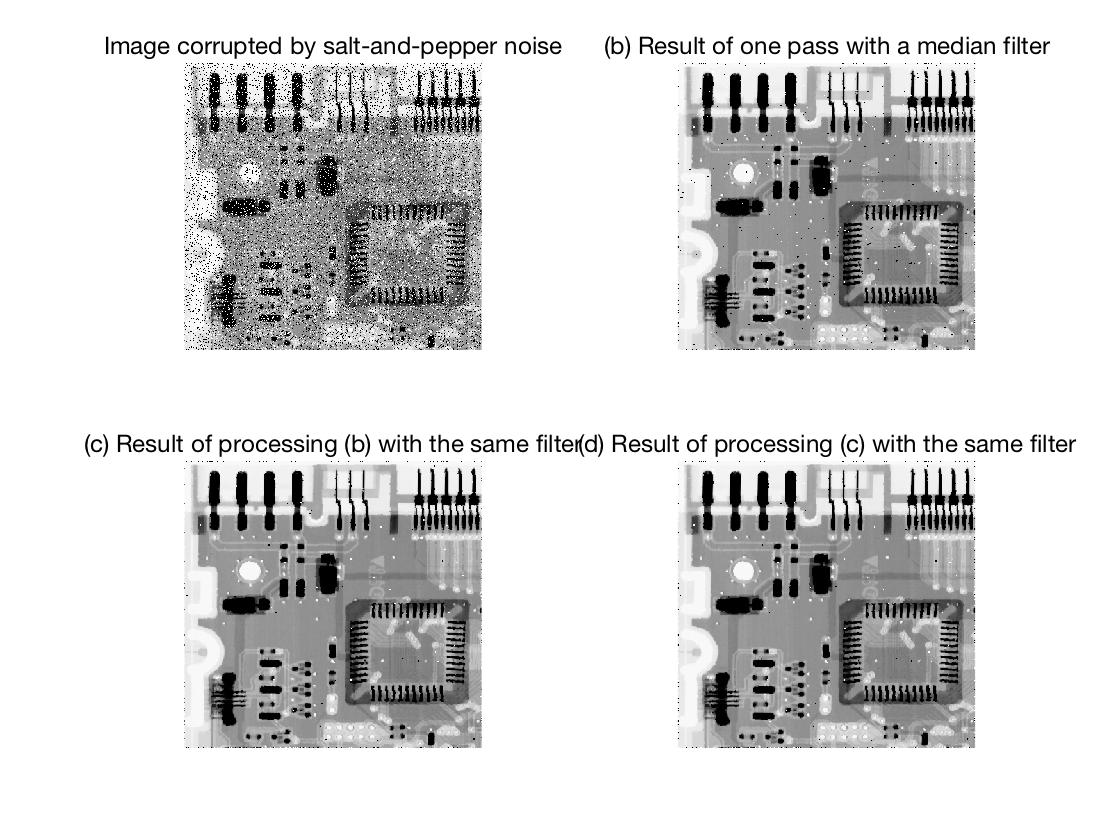
\includegraphics[width=1.0\textwidth]{images/4/order1.jpg}
   \caption{Original Book FIGURE 5.10}
\end{figure}
\begin{figure}[!htb]
   \centering  
   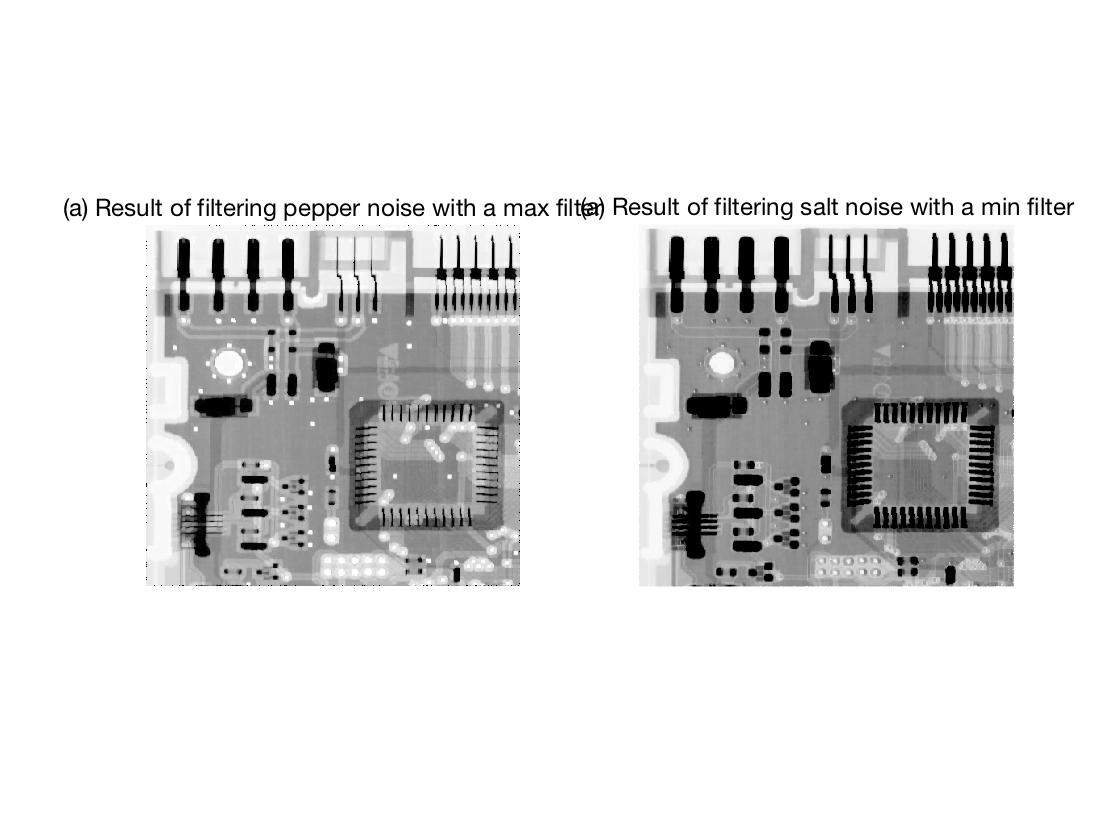
\includegraphics[width=0.7\textwidth]{images/4/order2.jpg}
   \caption{Original Book FIGURE 5.11}
\end{figure}
\begin{figure}[!htb]
   \centering  
   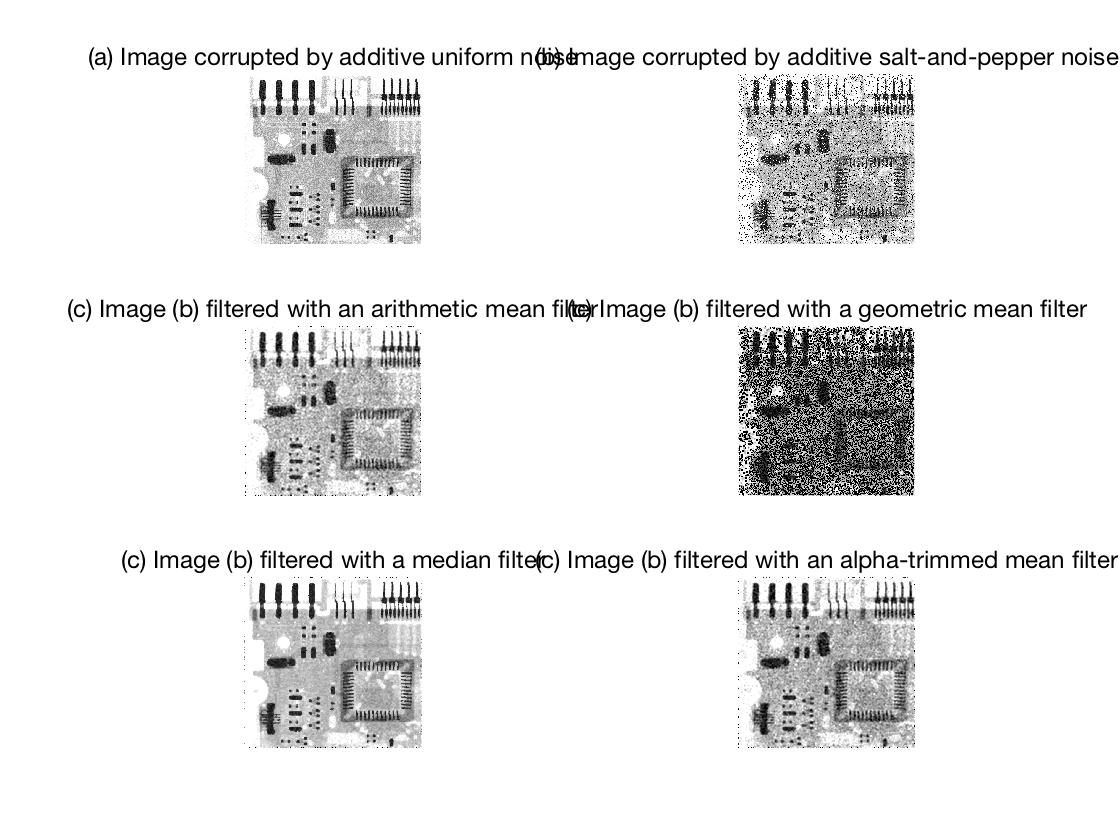
\includegraphics[width=1.0\textwidth]{images/4/order3.jpg}
   \caption{Original Book FIGURE 5.12}
\end{figure}
\newpage
\chapter{Image restoration}
\section{OverView}


\section{This is a section}
\subsection{This is a subsection}
\subsection{This is a subsection}



\chapter{Geometric transform}
\section{OverView}
Develop a geometric transform program that will rotate, translate, and scale an image by specified amounts, using the nearest neighbor and bilinear interpolation methods, respectively.

\section{Spatial Transformation}
\subsection{Rotate}
$(v, w)$ are pixel coordinates in the original image and $(x, y)$ are the corresponding pixel coordinates in the transformed image
\begin{align}
\left[               
  \begin{array}{ccc}  
    x & y & 1\\ 
  \end{array}
\right] 
=
\left[               
  \begin{array}{ccc}  
    v & w & 1\\ 
  \end{array}
\right]
T
=
\left[               
  \begin{array}{ccc}  
    v & w & 1\\ 
  \end{array}
\right]
\left[               
  \begin{array}{ccc}  
    cos\Theta & sin\Theta & 0\\
    -sin\Theta & cos\Theta & 0\\
    0 & 0 & 1\\ 
  \end{array}
\right]
\end{align}
\subsection{Results}
\begin{figure}[!htb]
   \centering  
   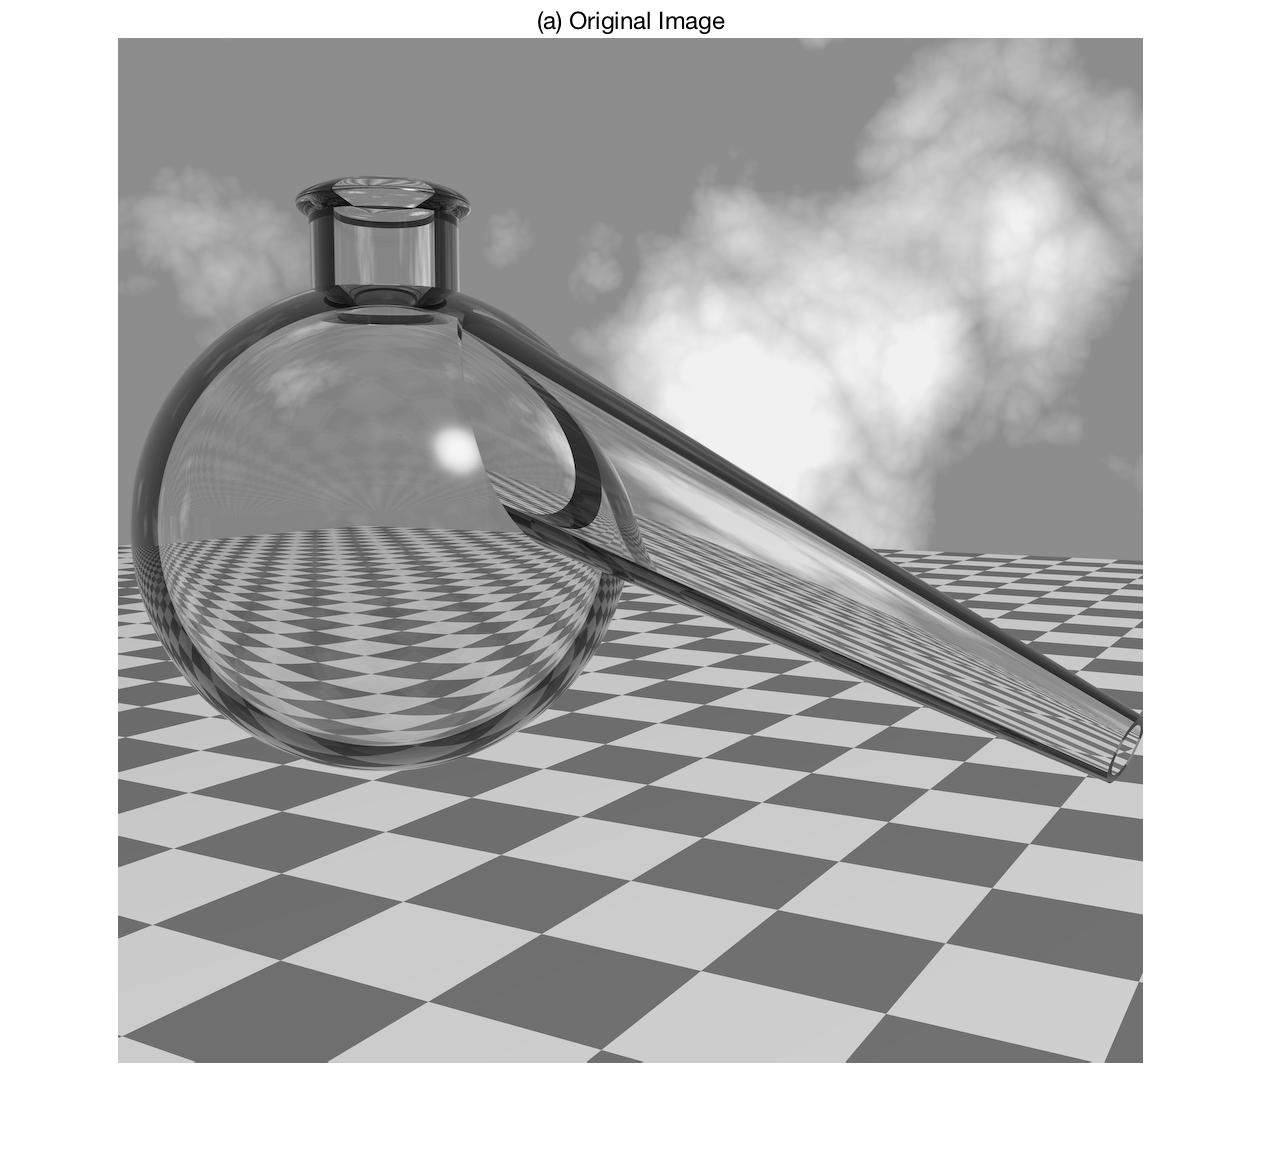
\includegraphics[width=0.8\textwidth]{images/6/rotate.jpg}
   \caption{Original Image}
\end{figure}
\newpage
\begin{figure}[!htb]
   \centering  
   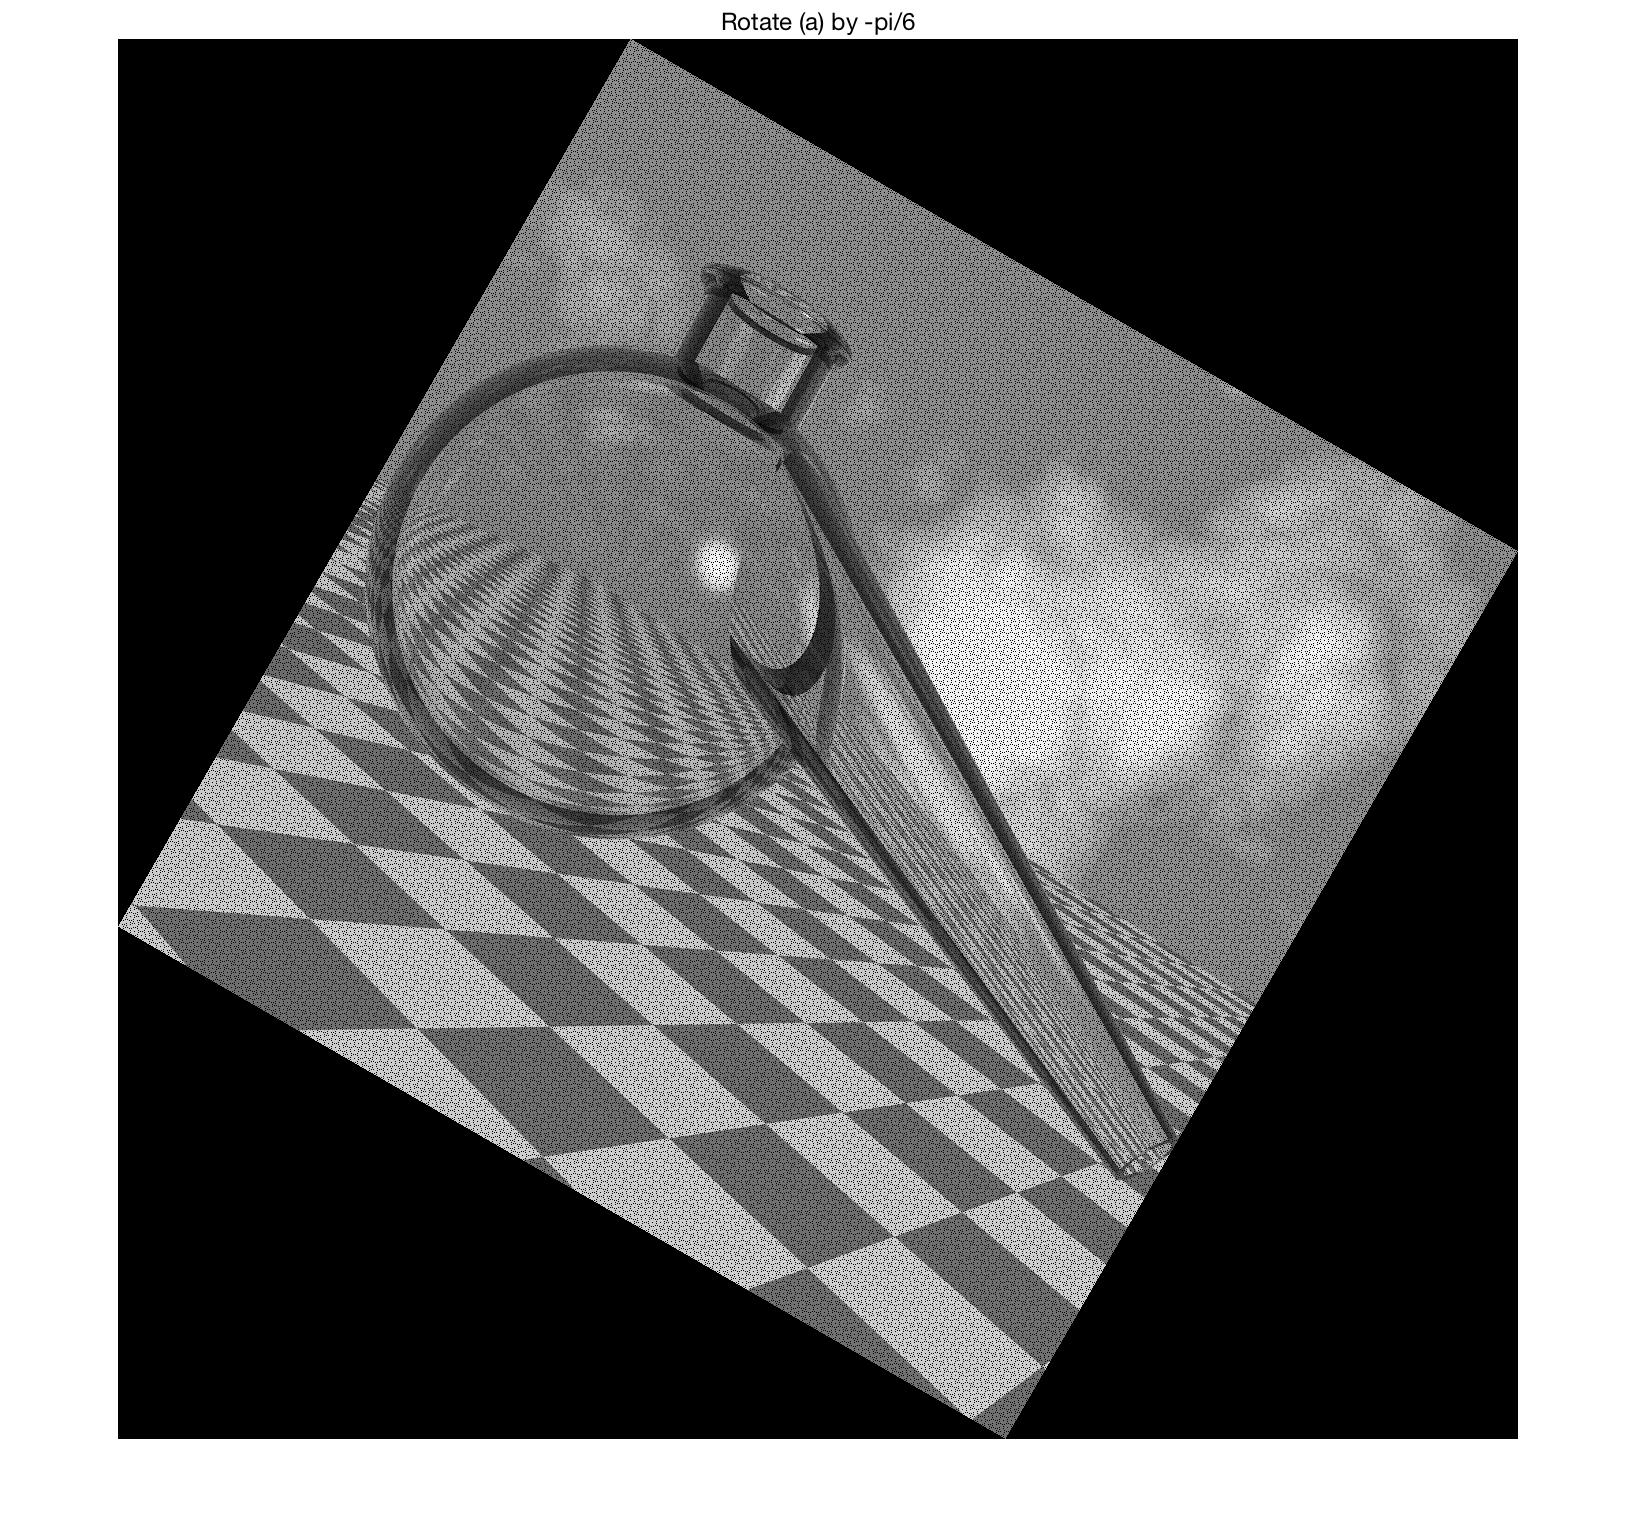
\includegraphics[width=0.7\textwidth]{images/6/rotate_pi.jpg}
   \caption{Rotate pi/6 without interpolation}
\end{figure}
\begin{figure}[!htb]
   \centering  
   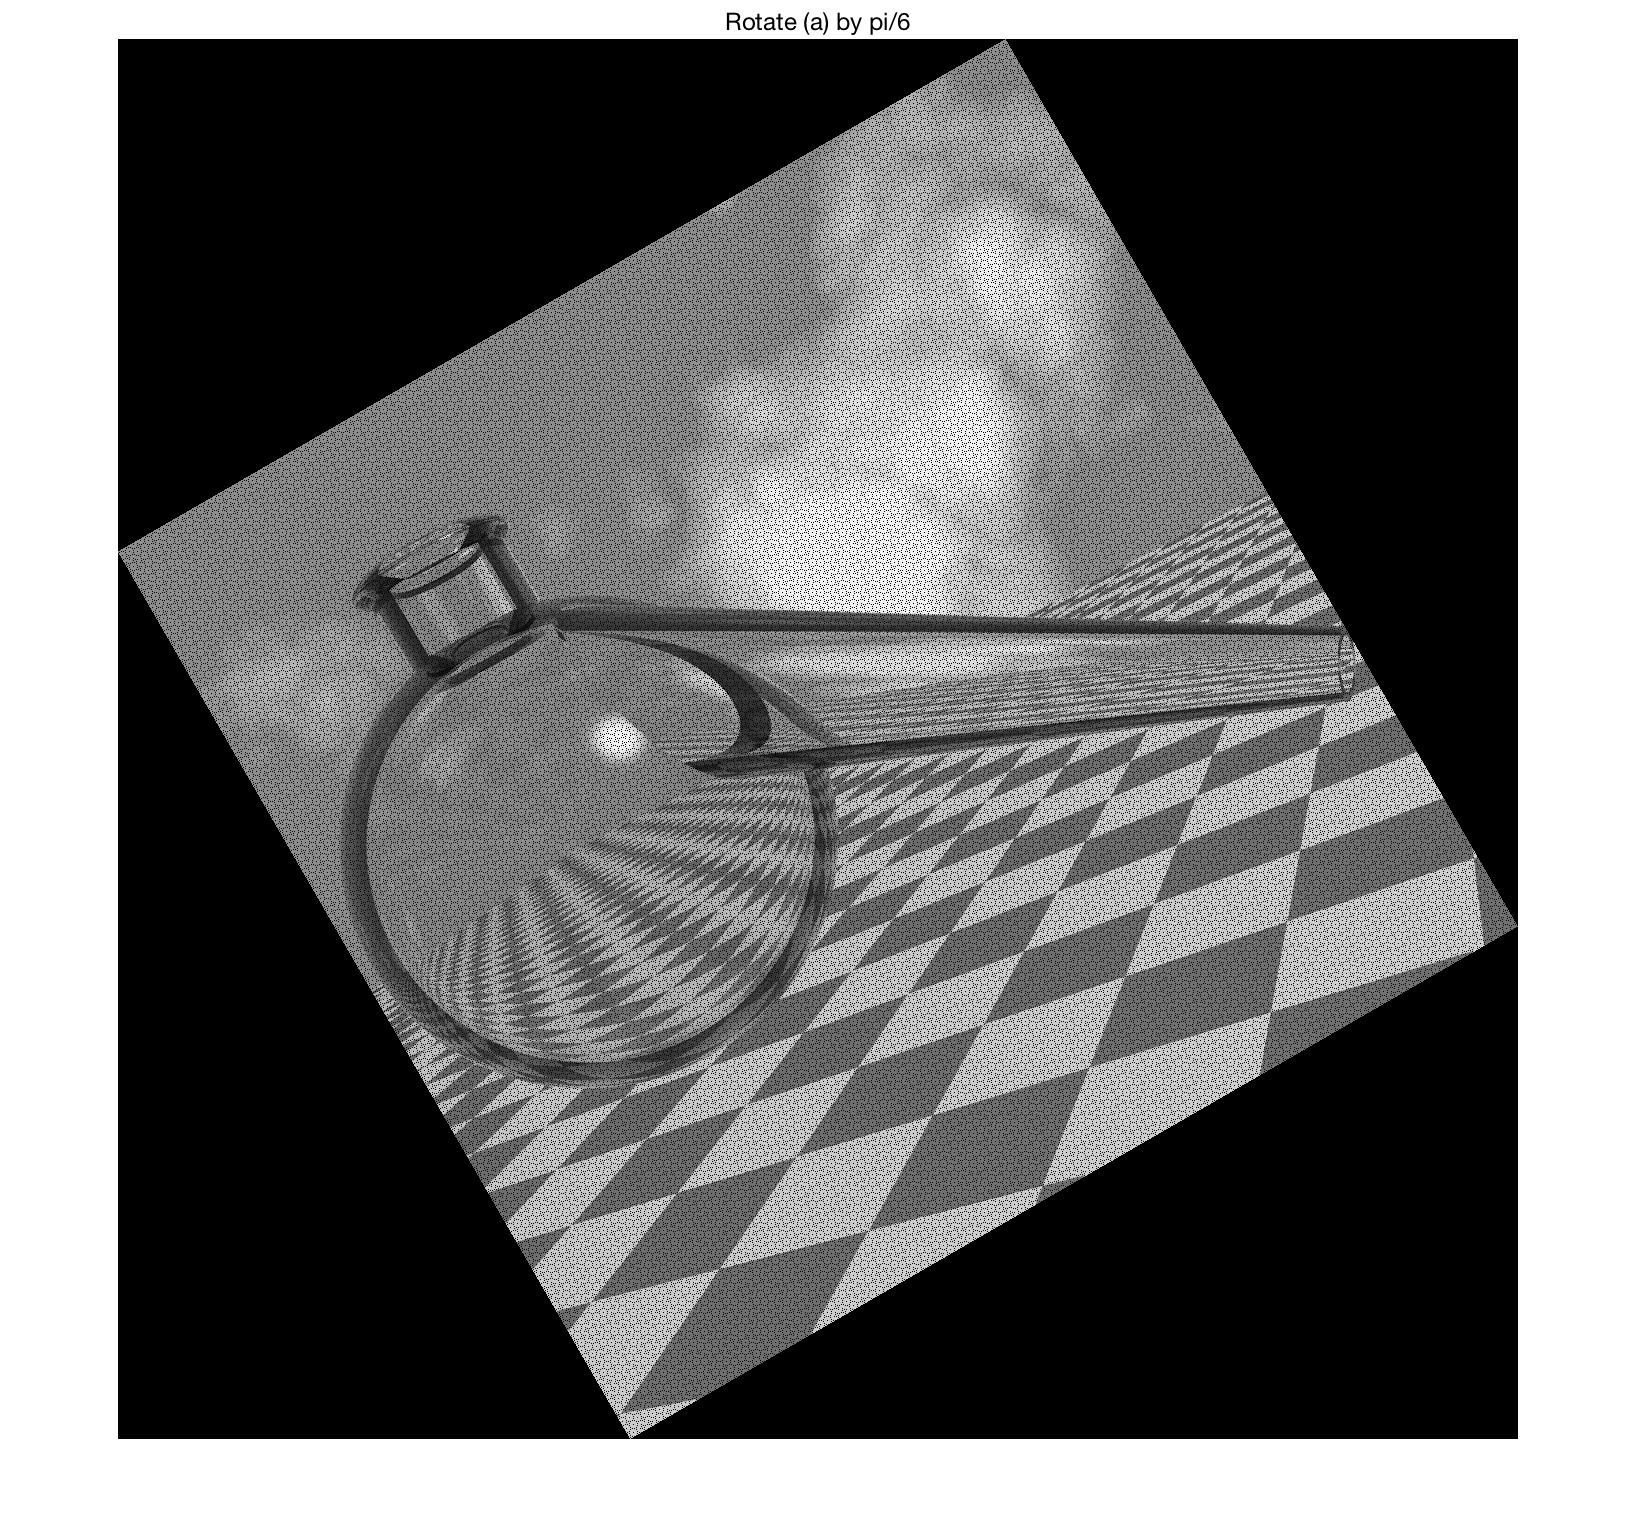
\includegraphics[width=0.7\textwidth]{images/6/rotate_pi_.jpg}
   \caption{Rotate -pi/6 without interpolation}
\end{figure}
\newpage

\subsection{Translate}
$(v, w)$ are pixel coordinates in the original image and $(x, y)$ are the corresponding pixel coordinates in the transformed image
\begin{align}
\left[               
  \begin{array}{ccc}  
    x & y & 1\\ 
  \end{array}
\right] 
=
\left[               
  \begin{array}{ccc}  
    v & w & 1\\ 
  \end{array}
\right]
T
=
\left[               
  \begin{array}{ccc}  
    v & w & 1\\ 
  \end{array}
\right]
\left[               
  \begin{array}{ccc}  
    1 & 0 & 0\\
    0 & 1 & 0\\
    t_x & t_y & 1\\ 
  \end{array}
\right]
\end{align}
\subsection{Results}
\begin{figure}[!htb]
   \centering  
   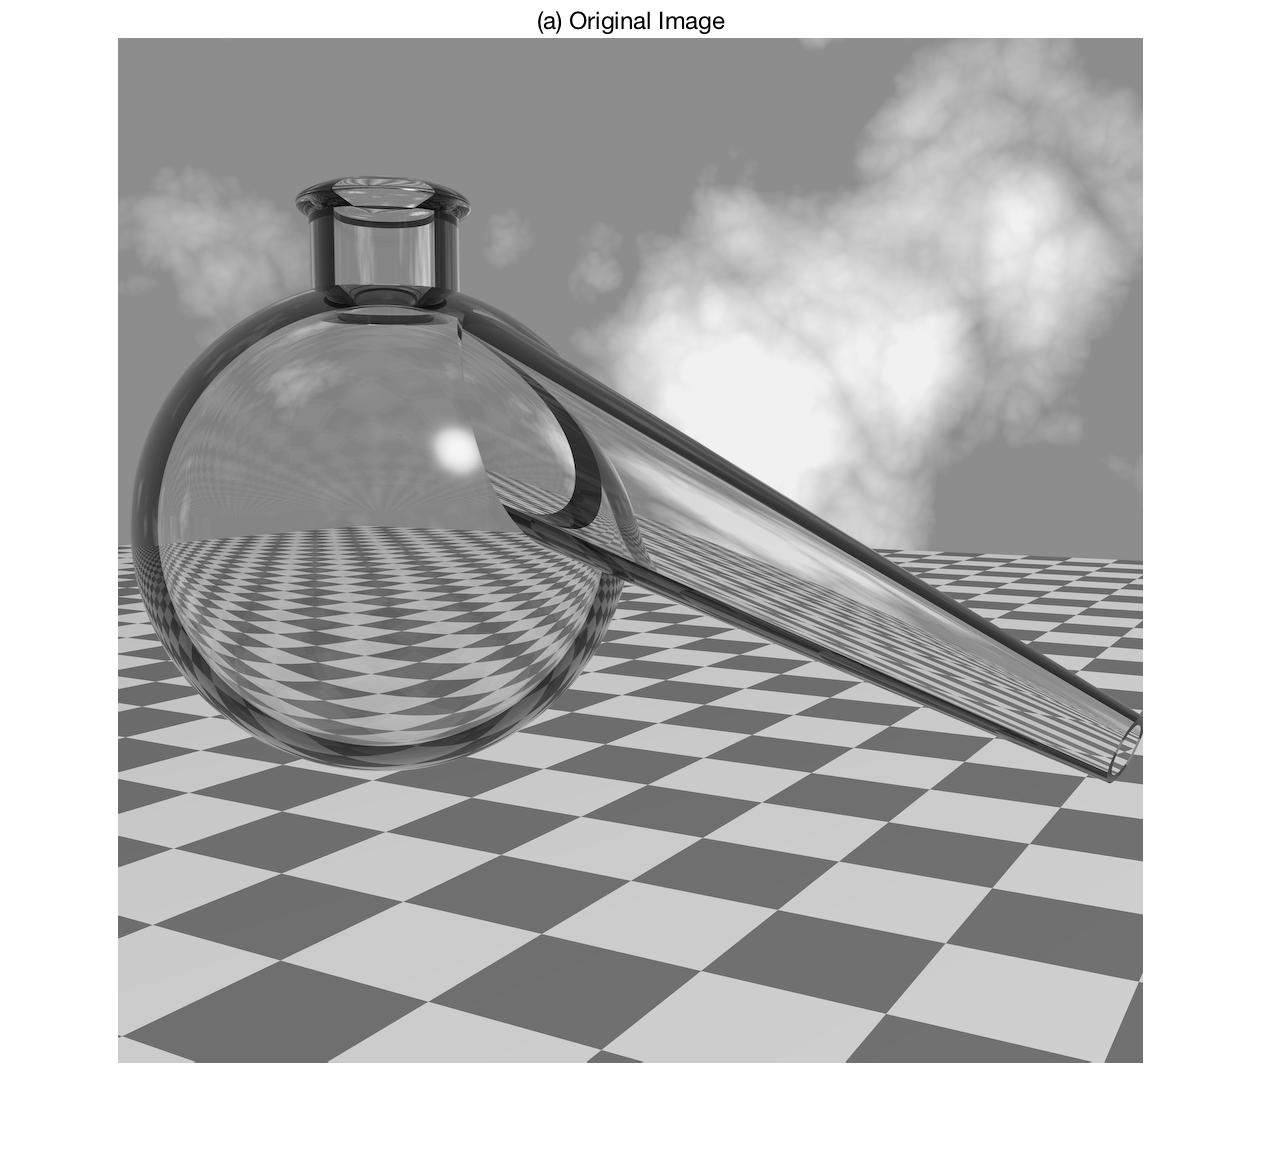
\includegraphics[width=1\textwidth]{images/6/translate.jpg}
   \caption{Original Image}
\end{figure}
\newpage
\begin{figure}[!htb]
   \centering  
   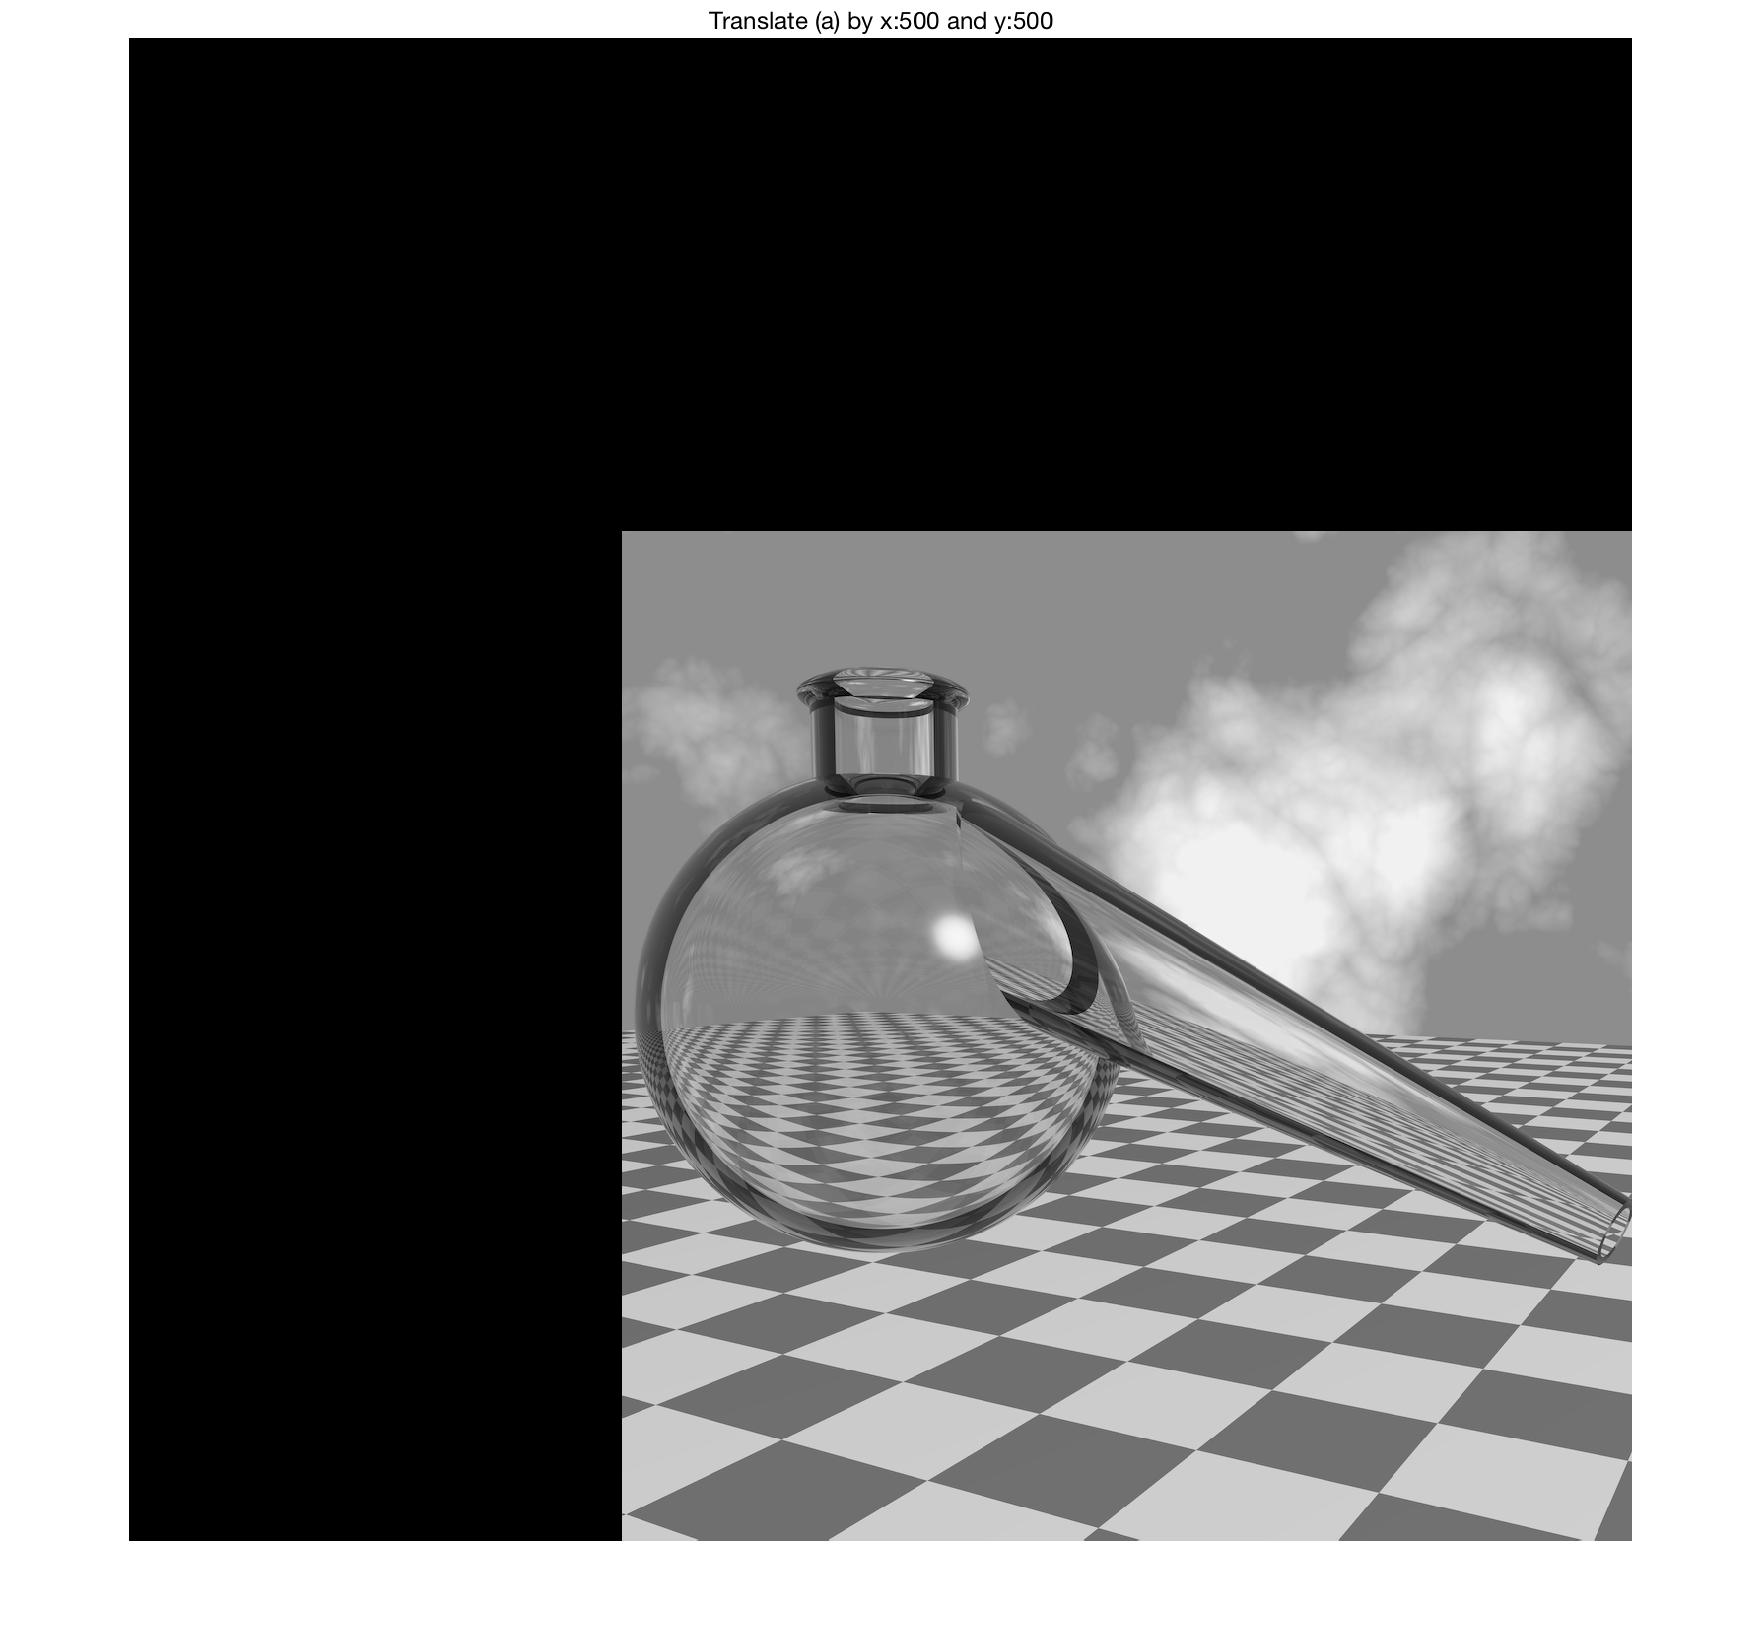
\includegraphics[width=0.7\textwidth]{images/6/translate_.jpg}
   \caption{Translate X:500 and Y:500}
\end{figure}
\begin{figure}[!htb]
   \centering  
   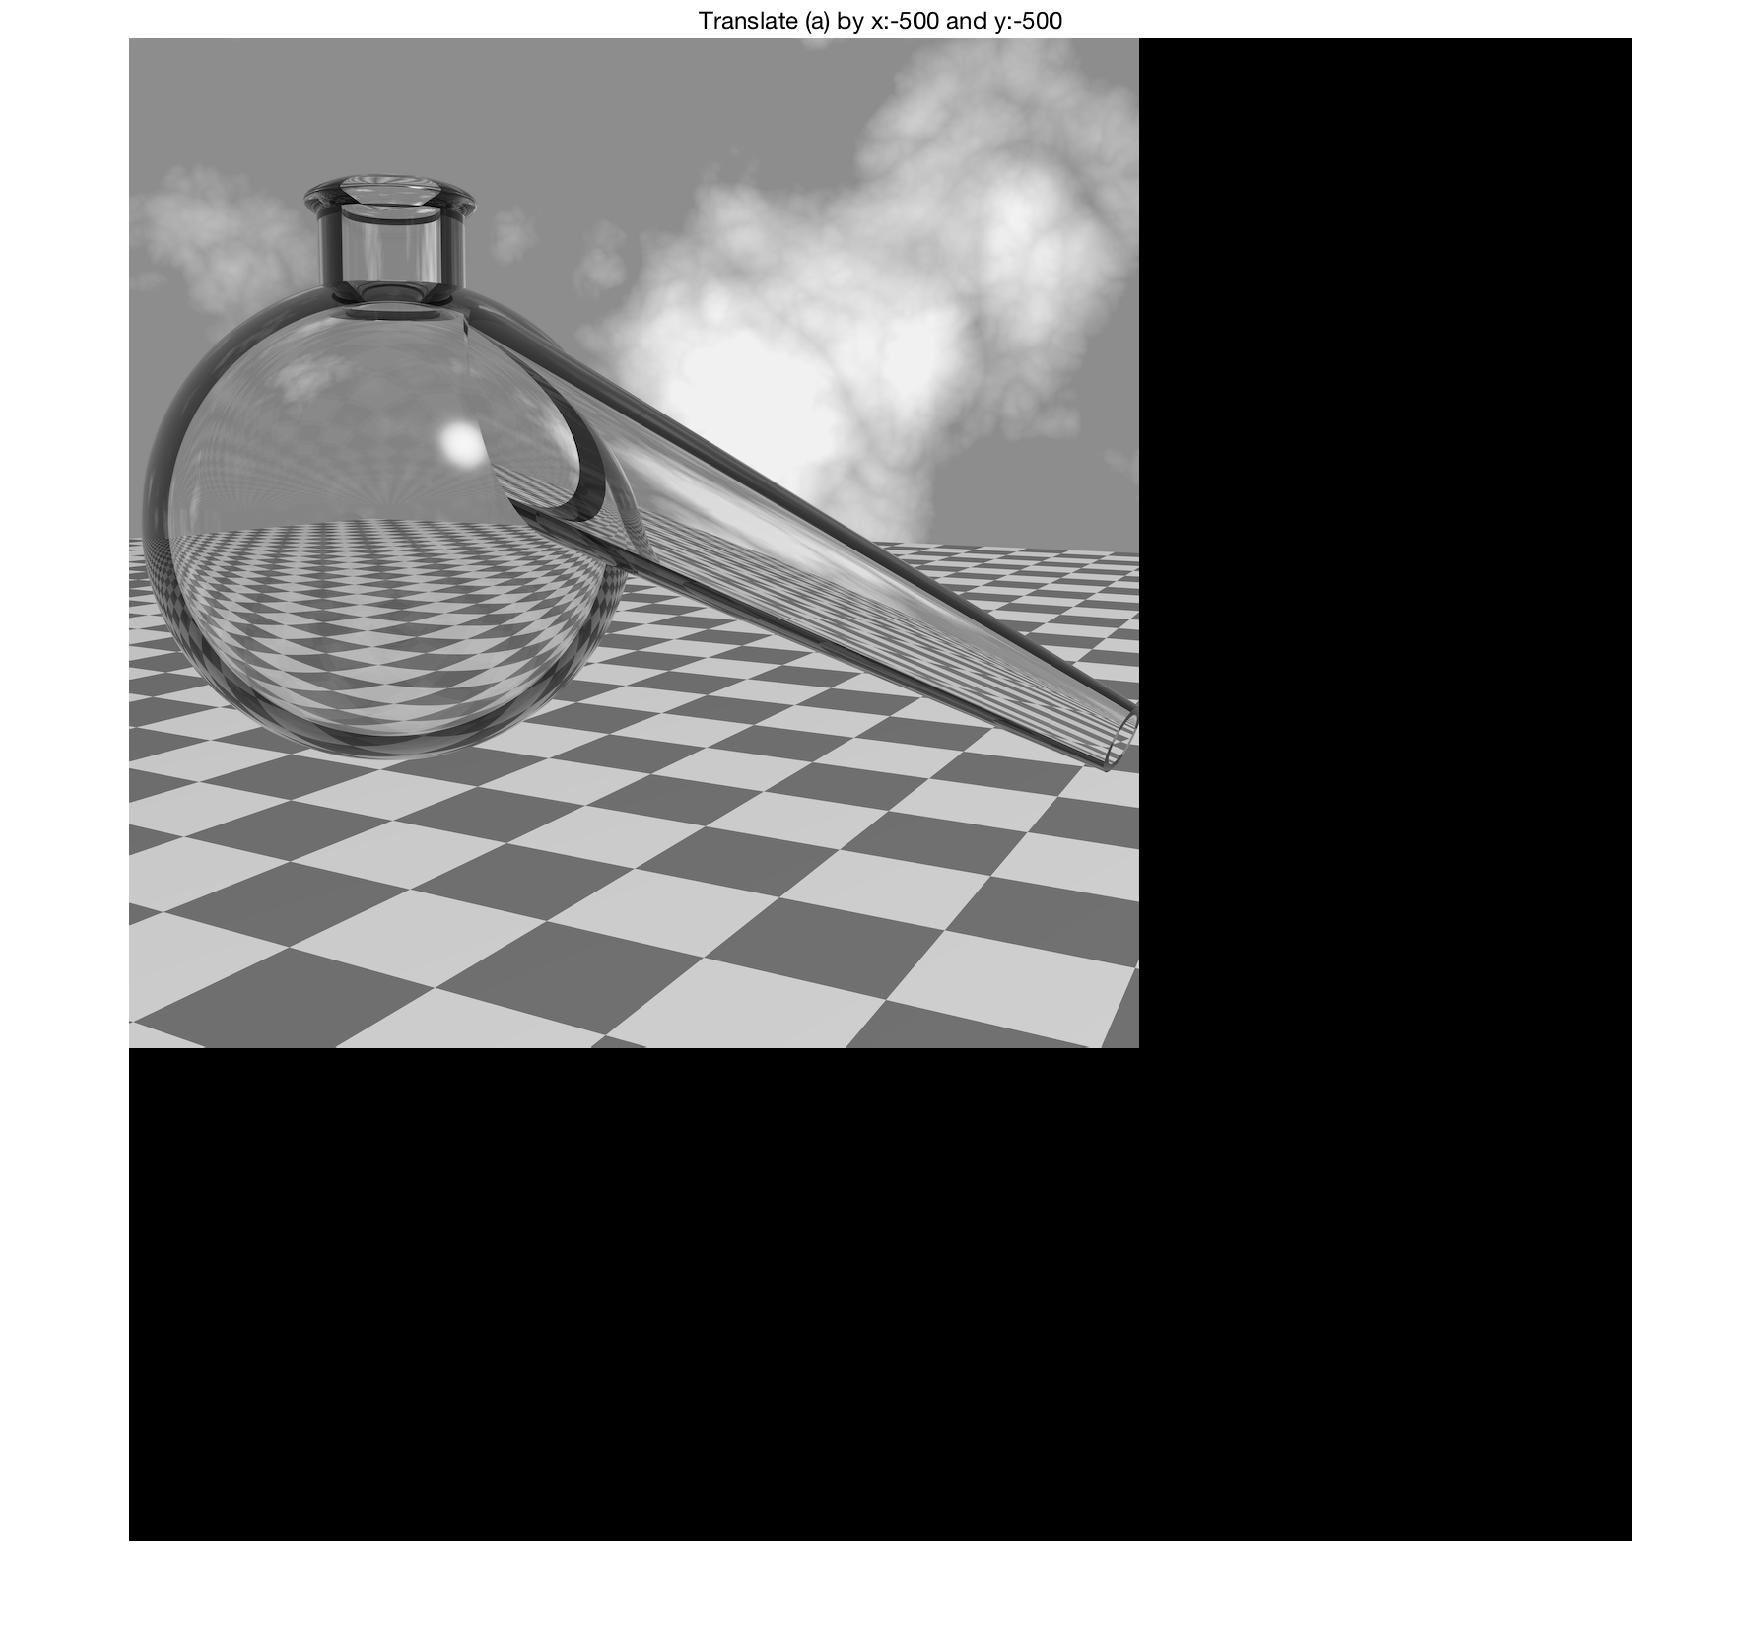
\includegraphics[width=0.7\textwidth]{images/6/translate__.jpg}
   \caption{Translate X:-500 and Y:-500}
\end{figure}
\newpage

\subsection{Scaling}
$(v, w)$ are pixel coordinates in the original image and $(x, y)$ are the corresponding pixel coordinates in the transformed image
\begin{align}
\left[               
  \begin{array}{ccc}  
    x & y & 1\\ 
  \end{array}
\right] 
=
\left[               
  \begin{array}{ccc}  
    v & w & 1\\ 
  \end{array}
\right]
T
=
\left[               
  \begin{array}{ccc}  
    v & w & 1\\ 
  \end{array}
\right]
\left[               
  \begin{array}{ccc}  
    c_x & 0 & 0\\
    0 & c_y & 0\\
    0 & 0 & 1\\ 
  \end{array}
\right]
\end{align}

\subsection{Results}
Since the original image is too large to show the detial change, I scale the original image to 0.25*0.25(b) and then scale (b) to 2*2.


\begin{figure}[!htb]
   \centering  
   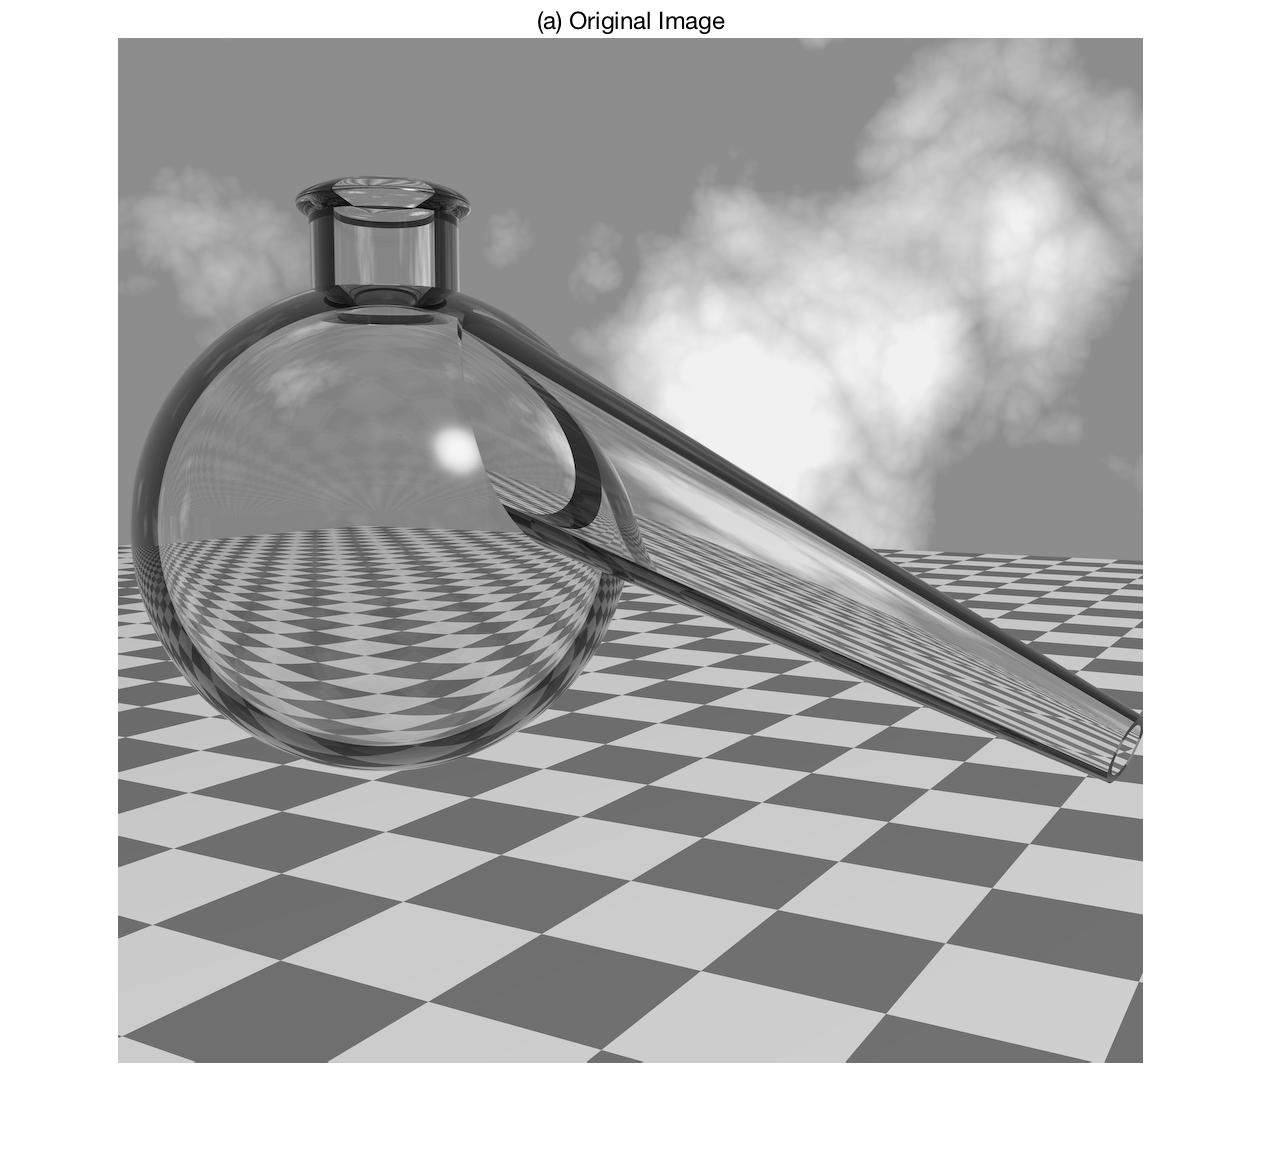
\includegraphics[width=1\textwidth]{images/6/scale.jpg}
   \caption{Original Image}
\end{figure}
\newpage
\begin{figure}[!htb]
   \centering  
   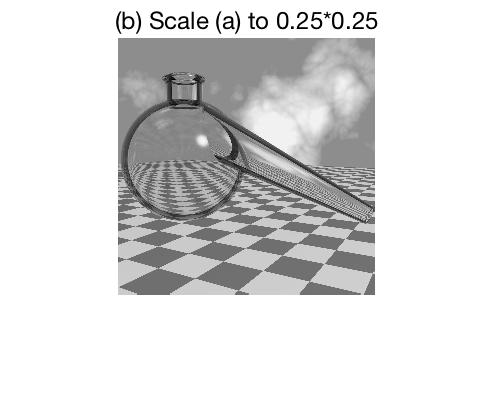
\includegraphics[width=0.7\textwidth]{images/6/scale_5.jpg}
   \caption{Scaling 0.25*0.25 without interpolation}
\end{figure}
\begin{figure}[!htb]
   \centering  
   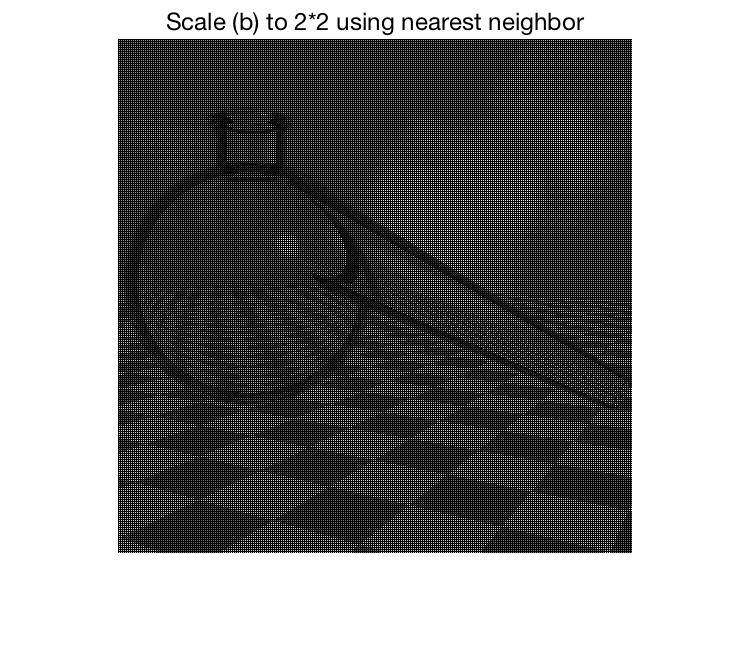
\includegraphics[width=0.7\textwidth]{images/6/scale_2.jpg}
   \caption{Scaling 2*2 without interpolation}
\end{figure}
\newpage

\section{Interpolation Methods}
\subsection{Methods}
\subsubsection{Nearest Neighbor Interpolation}
We look for its closest pixel in the original image and assign the intensity of that pixel to the new pixel.
\subsubsection{Bilinear Interpolation}
We use the four nearest neighbors to estimate the intensity at a given location.
\subsection{Results}
\begin{figure}[!htb]
   \centering  
   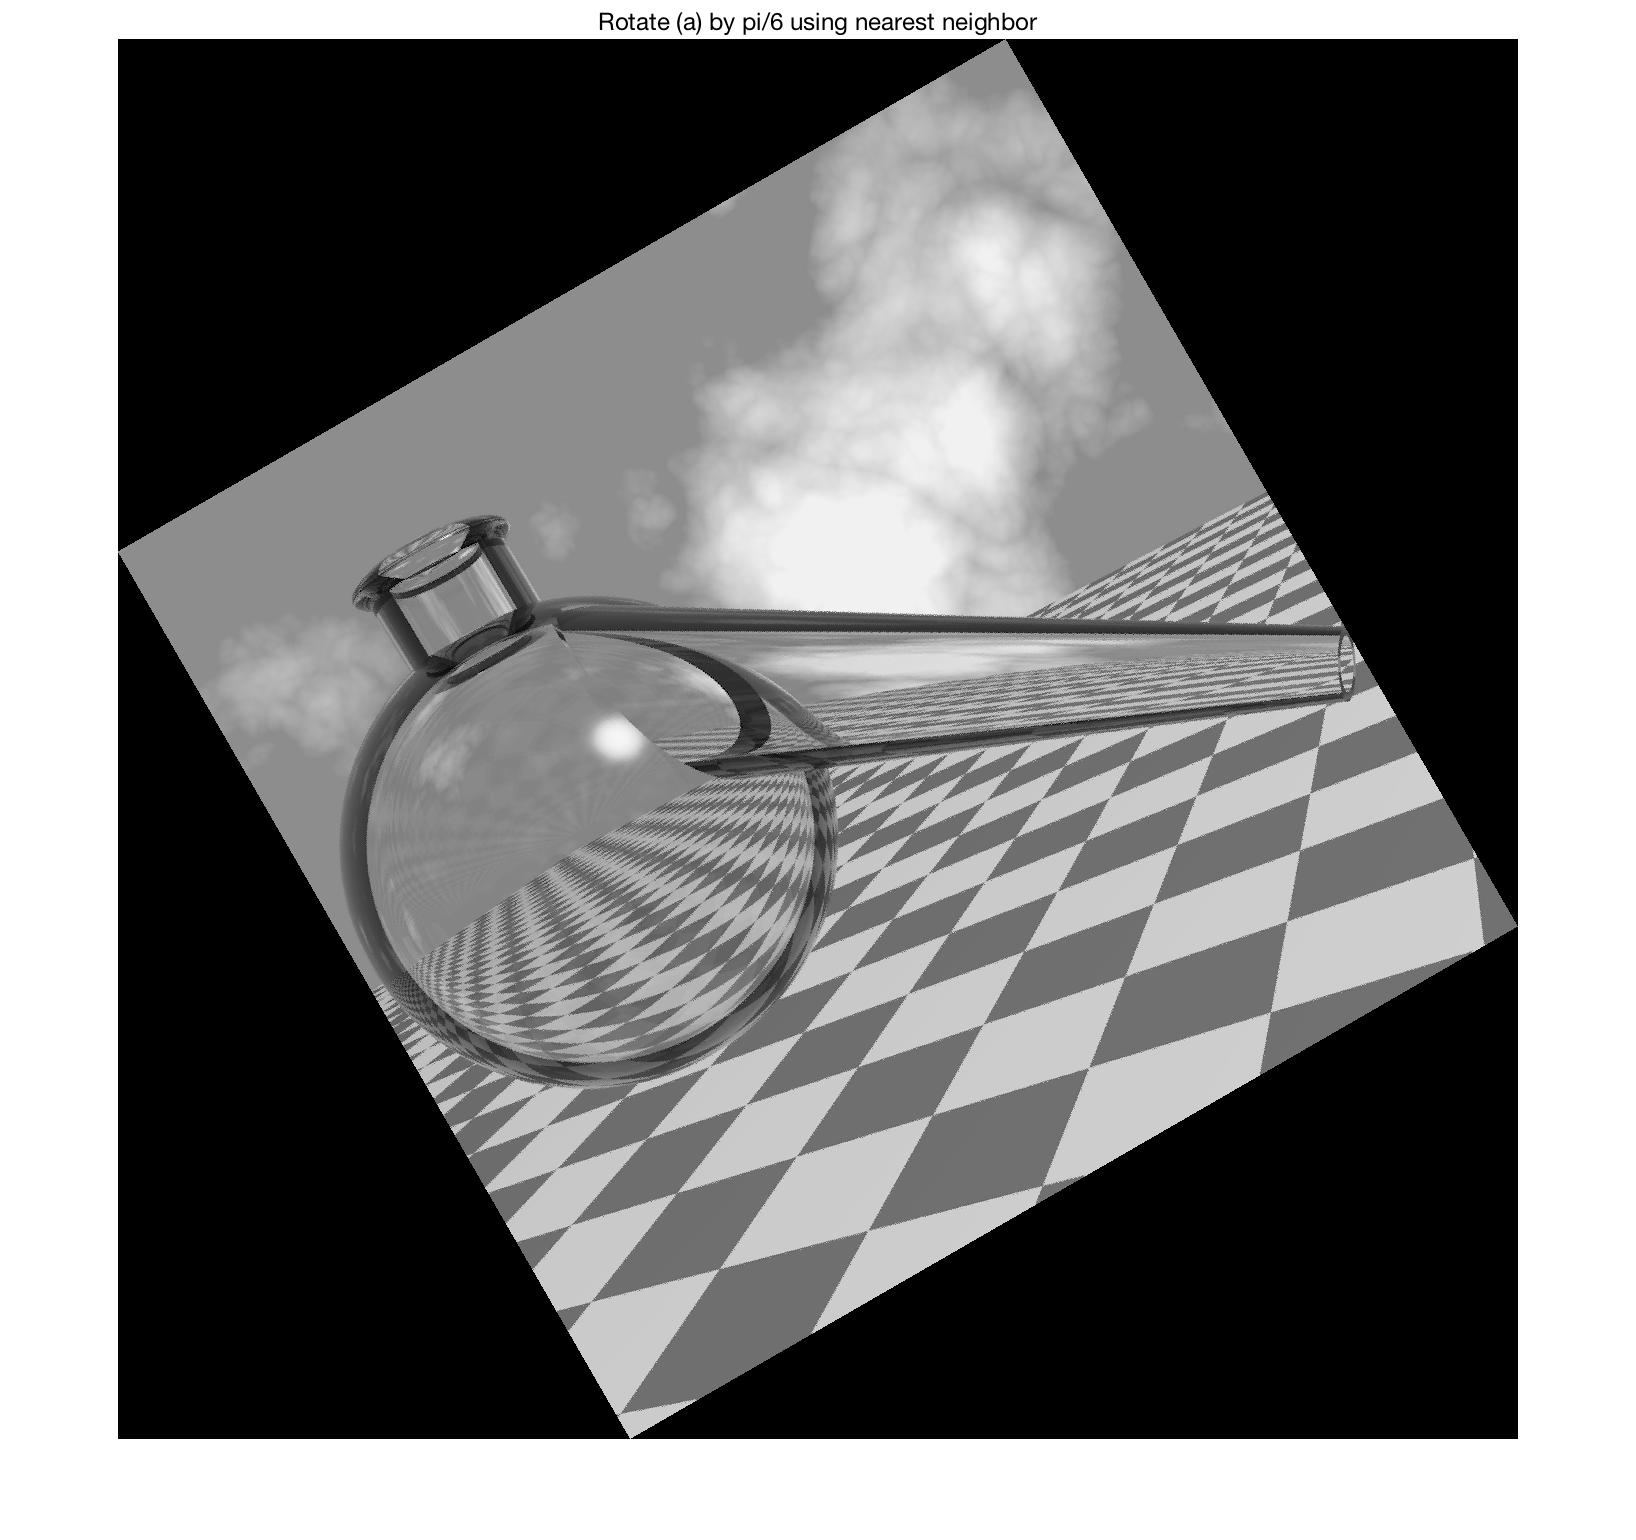
\includegraphics[width=1\textwidth]{images/6/rotate_nn.jpg}
   \caption{Rotate pi/6 using nearest neighbor interpolation}
\end{figure}

\begin{figure}[!htb]
   \centering  
   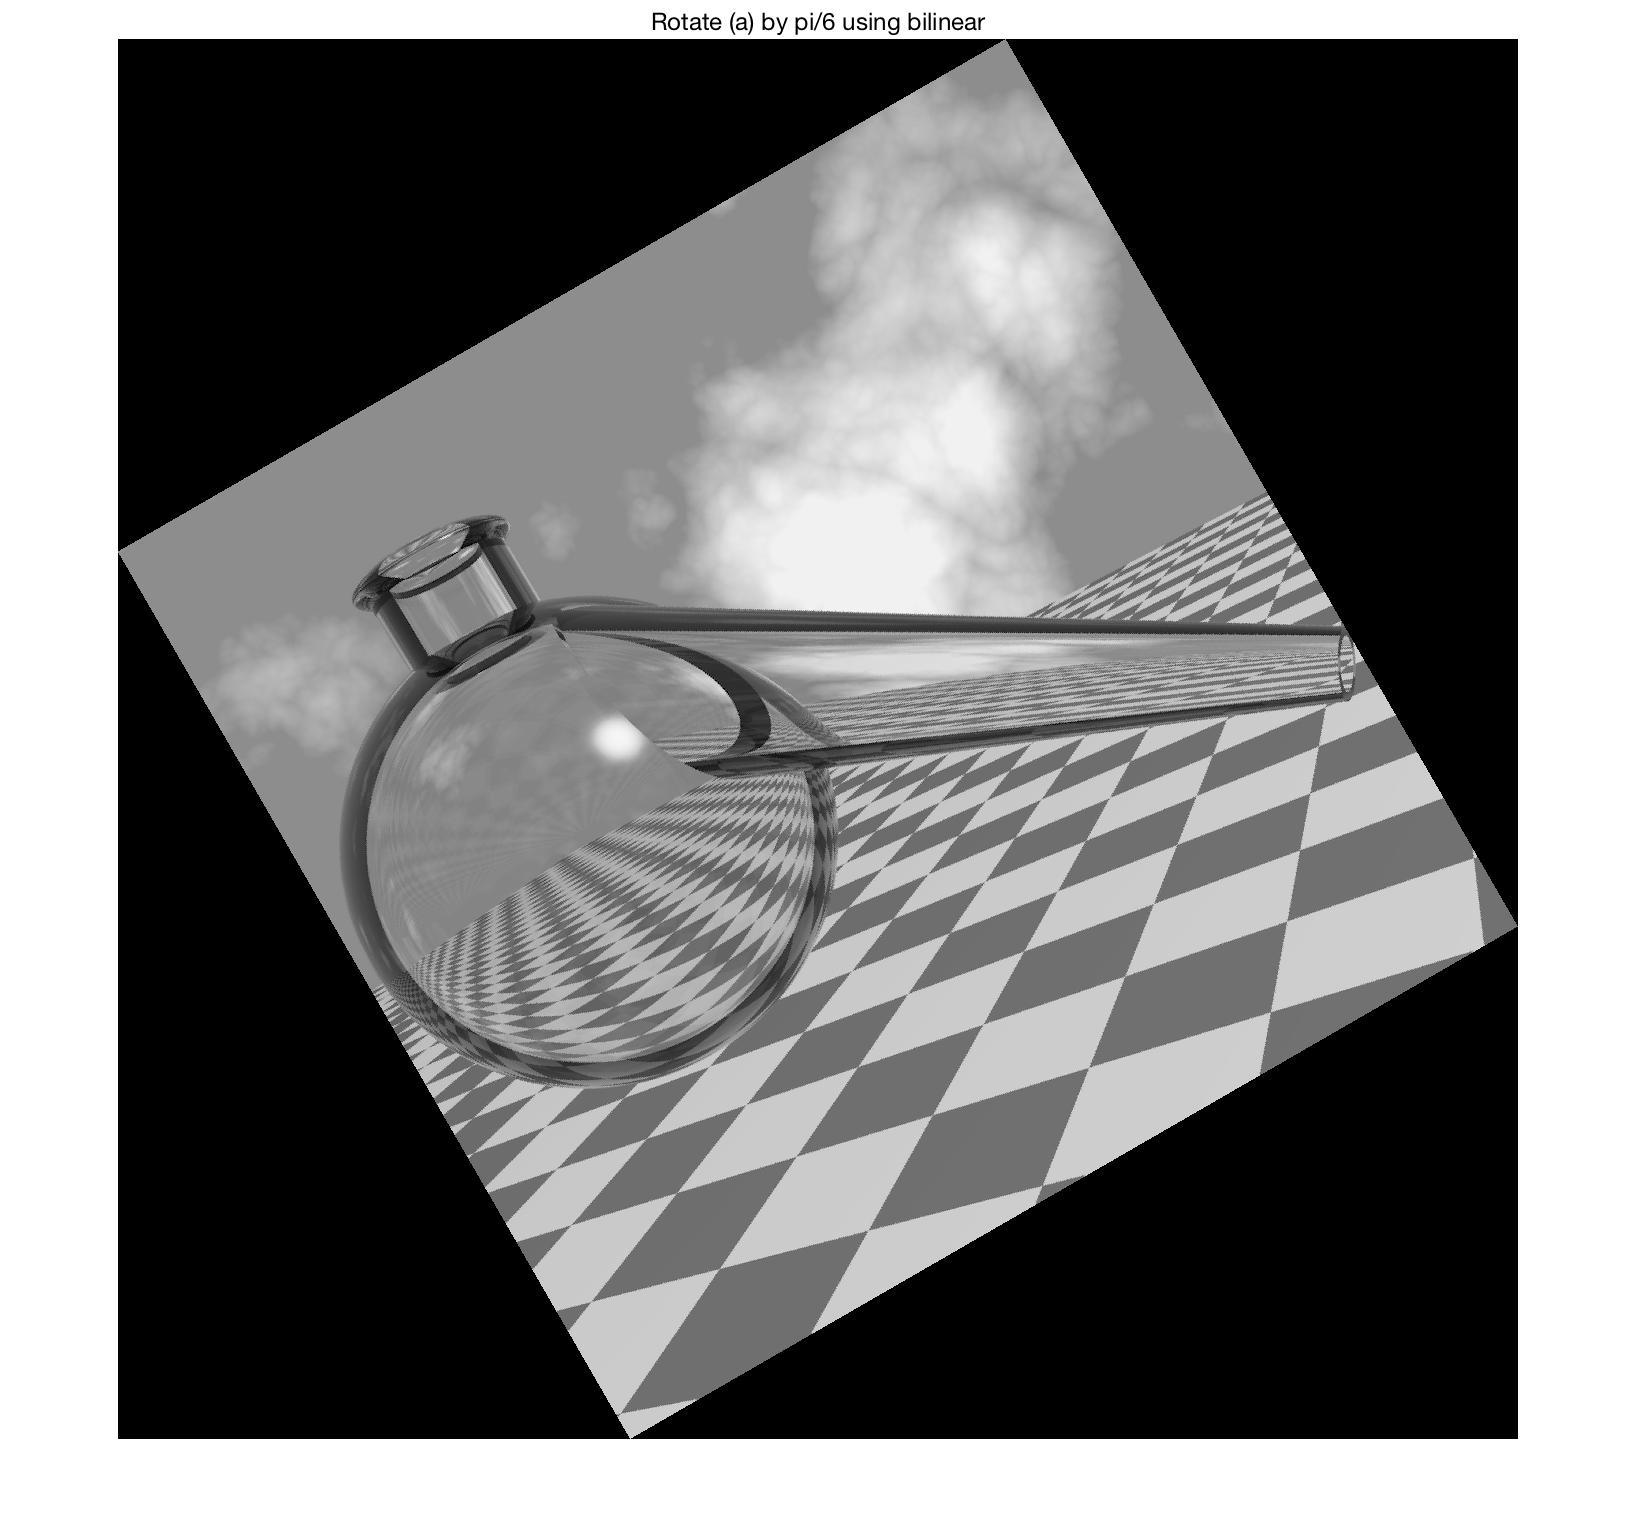
\includegraphics[width=0.7\textwidth]{images/6/rotate_b.jpg}
   \caption{Rotate pi/6 using bilinear interpolation}
\end{figure}

\begin{figure}[!htb]
   \centering  
   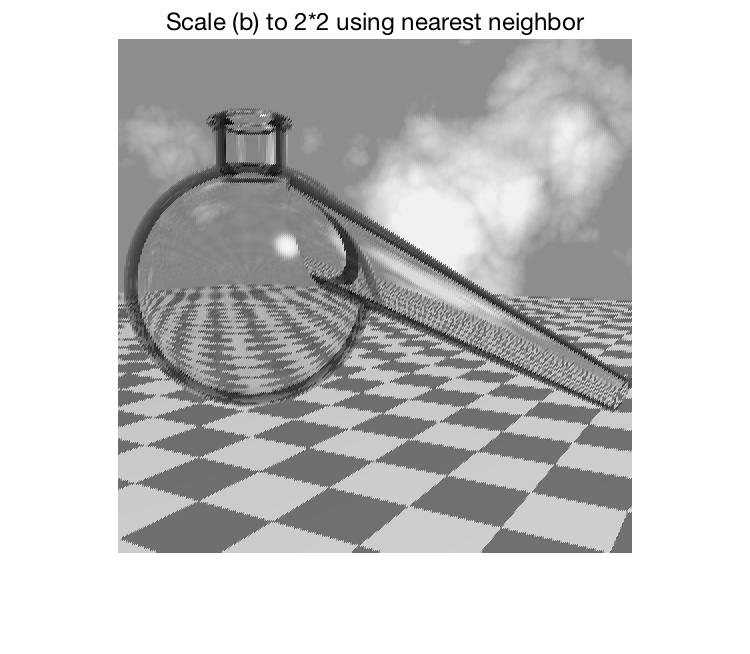
\includegraphics[width=0.7\textwidth]{images/6/scale_nn.jpg}
   \caption{Scaling 2*2 using nearest neighbor interpolation}
\end{figure}
\begin{figure}[!htb]
   \centering  
   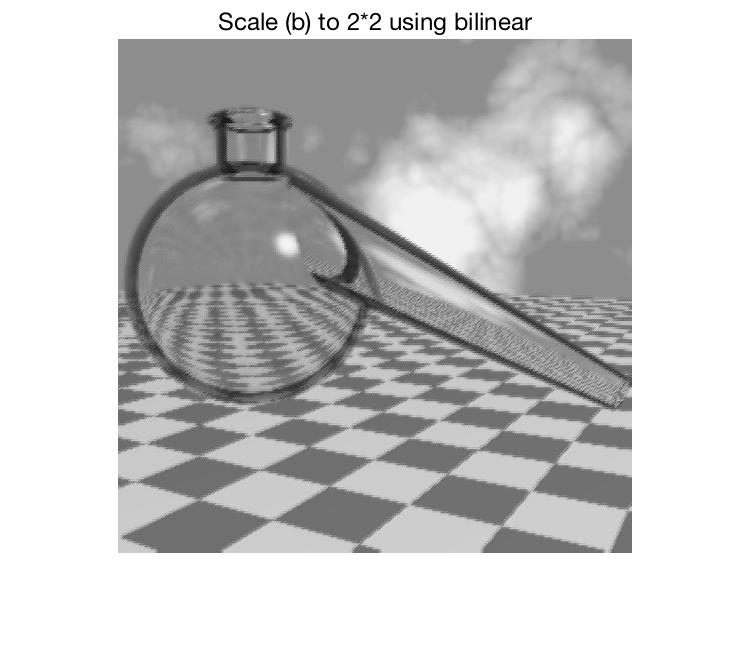
\includegraphics[width=1\textwidth]{images/6/scale_b.jpg}
   \caption{Scaling 2*2 using bilinear interpolation}
\end{figure}

\newpage

%%%%%%
\begin{appendices}
\chapter{Codes}
\section{Problem1}

\begin{lstlisting}[numbers=left, numberstyle=\tiny,keywordstyle=\color{blue!70},commentstyle=\color{red!50!green!50!blue!50},frame=shadowbox, rulesepcolor=\color{red!20!green!20!blue!20}] 
% Problem 1
% by Xue Fanyong
% Student ID:515030910443
% Histogram Equalizatio

%% Main Part
image1 = imread('Image Path/Fig1.jpg');
image2 = imread('Image Path/Fig2.jpg');

[histogram1,histogram_e1,transfer_f1,image_e1] = 
histogram_equalization(image1);
[histogram2,histogram_e2,transfer_f2,image_e2] = 
histogram_equalization(image2);

plot_data(image1,image_e1,histogram1,histogram_e1,transfer_f1);
plot_data(image2,image_e2,histogram2,histogram_e2,transfer_f2);

%% Functions Part

% get histogram of image
% image: get histogram of it
% histogram: the histogram of image
function histogram = get_histogram(image)
    histogram = zeros(256,1);
    [row,col]=size(image);
    for r = 1:row
        for c = 1:col
            gray = image(r,c);
            histogram(gray+1)=histogram(gray+1)+1;
        end
    end
end

% do the histogram_equalization for image
% image: do histogram_equalization for it
% histogram: original histogram; histogram_e: 
% histogram after histogram
% equalizatio; transfer_f: transfer function; 
% image_e: image after histogram
% equalizatio
function [histogram,histogram_e,transfer_f,image_e] = 
histogram_equalization(image)
    [row,col]=size(image);
    transfer_f = zeros(256,1);
    histogram = get_histogram(image);
    transfer_f(1) = 256*histogram(1)/(row*col);
    
    for i = 2:256
        transfer_f(i) = transfer_f(i-1)+255*histogram(i)/(row*col);
    end
    transfer_f = round(transfer_f);
    
    image_e = image;
    for r = 1:row
        for c = 1:col
            image_e(r,c)=transfer_f(image(r,c)+1);
        end
    end
    histogram_e = get_histogram(image_e);
end

% plot data
% image:original image; image_e: 
% image after histogram equalizatio; 
% histogram: original histogram; 
% histogram_e: histogram after histogram equalizatio;
% transfer_f: transfer function
function plot_data(image,image_e,histogram,histogram_e,transfer_f)
    figure();
    subplot(2,3,1);
    imshow(image);
    title("Original Image");
    subplot(2,3,2);
    imshow(image_e);
    title("Image(Histogram Equalization)");
    subplot(2,3,3);
    bar(histogram);
    title("Histogram");
    subplot(2,3,4);
    bar(histogram_e);
    title("Histogram(Equalization)");
    subplot(2,3,5);
    plot(transfer_f);
    title("Transfer Funciton");
end

\end{lstlisting}


\section{Problem 2}

\begin{lstlisting}[numbers=left, numberstyle=\tiny,keywordstyle=\color{blue!70},commentstyle=\color{red!50!green!50!blue!50},frame=shadowbox, rulesepcolor=\color{red!20!green!20!blue!20}] 
% Problem 2
% by Xue Fanyong
% Student ID:515030910443
% Combining spatial enhancement methods

%% Main Part
image = imread('Image Path/skeleton_orig.tif');
[row,col] = size(image);
mask = [-1 -1 -1;-1 8 -1;-1 -1 -1];
mask = double(mask);
b_image = laplace_transformations(image,mask);
c_image = b_image+im2double(image);
d_image = sobel_gradient(image);
e_image = smooth(d_image);
f_image = im2double(e_image).*c_image;
g_image = abs(f_image)+im2double(image);
h_image = sqrt(g_image);
plot_data(image,b_image,c_image,d_image,
          e_image,f_image,g_image,h_image);

%% Function Part

% Laplace Transfromation for image using mask
% Input:
%   image:image you want to perform
%   mask:Laplace mask you want to use
% Output:
%   image_l:image after laplace transformation

function image_l = laplace_transformations(image,mask)
    [row,col] = size(image);
    mask = double(mask);
    %append image
    image_l = im2double(image);
    image = [zeros(row,2) image zeros(row,2)];
    image = [zeros(2,col+4);image;zeros(2,col+4)];
    image_append = im2double(image);
    
    for r = 1:row
        for c = 1:col
            image_l(r,c) = sum(sum(image_append(r:r+2,c:c+2).*mask));
        end
    end
end
%{
    sobel gradient for image
%}
function image_s = sobel_gradient(image)
    [row,col] = size(image);
    x_mask = [-1 -2 -1;0 0 0;1 2 1];
    y_mask = [-1 0 1;-2 0 2;-1 0 1];
    image_s = image;
    image = double(image);
    
    for r = 2:row-1
        for c = 2:col-1
            image_s(r,c) = 
            abs(sum(sum(image(r-1:r+1,c-1:c+1).*x_mask)))+
            abs(sum(sum(image(r-1:r+1,c-1:c+1).*y_mask)));
        end
    end
end
%{
    smooth image using 5*5 mean filter
%}
function image_s = smooth(image)
    [row,col] = size(image);
    image_s = image;
    for r = 3:row-2
        for c = 3:col-2
            image_s(r,c) = mean(mean(image(r-2:r+2,c-2:c+2)));
        end
    end
end
%{
    plot data
%}
function plot_data(a,b,c,d,e,f,g,h)
    figure();
    
    subplot(241);
    imshow(a);
    title('(a) Oringinal Image');
    
    subplot(242);
    imshow(b,[]);
    title('(b) Laplacian of (a)');
    
    subplot(245);
    imshow(c,[]);
    title('(c) Sharpened image');
    
    subplot(246);
    imshow(d);
    title('(d) Sobel gradient');
    
    subplot(243);
    imshow(e);
    title('(e) Smoothed sobel image');
    
    subplot(244);
    imshow(f,[]);
    title('(f) Product of (c) and (e)');
    
    subplot(247);
    imshow(g,[]);
    title('(g) Sharpened image');
    
    subplot(248);
    imshow(h,[]);
    title('(h) Final result');
end

\end{lstlisting}


\section{Problem 3}

\begin{lstlisting}[numbers=left, numberstyle=\tiny,keywordstyle=\color{blue!70},commentstyle=\color{red!50!green!50!blue!50},frame=shadowbox, rulesepcolor=\color{red!20!green!20!blue!20}] 
%{
    Problem 3
    by Fanyong Xue 
    Student ID:515030910443
    Filtering in frequency domain
    
%}

%% Main Part
image = imread('Image Path/characters_test_pattern.tif');

ideal_low_plot_data(image);
ideal_high_plot_data(image);
butterworth_low_plot_data(image);
butterworth_high_plot_data(image);
gaussian_low_plot_data(image);
gaussian_high_plot_data(image);


%% Function Part

% Ideal
function ideal_high_plot_data(image)

    figure('name','Ideal High Pass');
    
    subplot(321);
    imshow(image);
    title('Original Image');
    
    subplot(322);
    imshow(IHPF(image,10),[]);
    title('Radius = 10');
    
    subplot(323);
    imshow(IHPF(image,30),[]);
    title('Radius = 30');
    
    subplot(324);
    imshow(IHPF(image,60),[]);
    title('Radius = 60');
    
    subplot(325);
    imshow(IHPF(image,160),[]);
    title('Radius = 160');
    
    subplot(326);
    imshow(IHPF(image,460),[]);
    title('Radius = 460');
    
end
function ideal_low_plot_data(image)

    figure('name','Ideal Low Pass');
    
    subplot(321);
    imshow(image);
    title('Original Image');
    
    subplot(322);
    imshow(ILPF(image,10),[]);
    title('Radius = 10');
    
    subplot(323);
    imshow(ILPF(image,30),[]);
    title('Radius = 30');
    
    subplot(324);
    imshow(ILPF(image,60),[]);
    title('Radius = 60');
    
    subplot(325);
    imshow(ILPF(image,160),[]);
    title('Radius = 160');
    
    subplot(326);
    imshow(ILPF(image,460),[]);
    title('Radius = 460');
    
end
function image_i = ILPF(image,radius)
    
    fliter = ILPF_fliter(image,radius);
    image_i = transfer(image,fliter);
    %{
    image_f = fft2(image,2*row,2*col);
    image_f = fftshift(image_f);
    %image_f = log(1+abs(image_f));
    
    %%%%%%%
    image_i = image_f.*fliter;
    
    image_i = ifftshift(image_i);
    image_i = ifft2(image_i);
    
    %image_i = abs(image_i);
    image_i = image_i(1:row,1:col);
    image_i = real(image_i);
    image_f = log(1+abs(image_f));
    %}
end
function image_i = IHPF(image,radius)
    fliter = 1-ILPF_fliter(image,radius);
    image_i = transfer(image,fliter);
end
function fliter = ILPF_fliter(image,radius)
    [row,col]=size(image);
    fliter = zeros(2*row,2*col);
    
    for r = 1:2*row
        for c = 1:2*col
            if sqrt((r-row)^2+(c-col)^2) <= radius
                fliter(r,c) = 1;
            end
        end
    end
end


% Butterworth
function butterworth_low_plot_data(image)
    figure('name','Butterworth Low Pass');
    
    subplot(321);
    imshow(image);
    title('Original Image');
    
    subplot(322);
    imshow(BLFP(image,2,10),[]);
    title('n=2,Radius = 10');
    
    subplot(323);
    imshow(BLFP(image,2,30),[]);
    title('n=2,Radius = 30');
    
    subplot(324);
    imshow(BLFP(image,2,60),[]);
    title('n=2,Radius = 60');
    
    subplot(325);
    imshow(BLFP(image,2,160),[]);
    title('n=2,Radius = 160');
    
    subplot(326);
    imshow(BLFP(image,2,460),[]);
    title('n=2,Radius = 460');
    
end
function butterworth_high_plot_data(image)
    figure('name','Butterworth High Pass');
    
    subplot(321);
    imshow(image);
    title('Original Image');
    
    subplot(322);
    imshow(BHFP(image,2,10),[]);
    title('n=2,Radius = 10');
    
    subplot(323);
    imshow(BHFP(image,2,30),[]);
    title('n=2,Radius = 30');
    
    subplot(324);
    imshow(BHFP(image,2,60),[]);
    title('n=2,Radius = 60');
    
    subplot(325);
    imshow(BHFP(image,2,160),[]);
    title('n=2,Radius = 160');
    
    subplot(326);
    imshow(BHFP(image,2,460),[]);
    title('n=2,Radius = 460');
    
end
function image_b = BLFP(image, n,radius)
    
    fliter = BLFP_fliter(image, n,radius);
    image_b = transfer(image,fliter);
    
end
function image_b = BHFP(image, n,radius)
    
    fliter = 1-BLFP_fliter(image, n,radius);
    image_b = transfer(image,fliter);
    
end
function fliter = BLFP_fliter(image, n,radius)
    [row,col]=size(image);
    fliter = zeros(2*row,2*col);
    
    for r = 1:2*row
        for c = 1:2*col
            fliter(r,c) = 1/(1+(sqrt((r-row)^2+
                      (c-col)^2)/radius)^(2*n));
        end
    end
end

% Gaussian
function gaussian_low_plot_data(image)
    figure('name','Gaussian Low Pass');
    
    subplot(321);
    imshow(image);
    title('Original Image');
    
    subplot(322);
    imshow(GLFP(image,10),[]);
    title('Radius = 10');
    
    subplot(323);
    imshow(GLFP(image,30),[]);
    title('Radius = 30');
    
    subplot(324);
    imshow(GLFP(image,60),[]);
    title('Radius = 60');
    
    subplot(325);
    imshow(GLFP(image,160),[]);
    title('Radius = 160');
    
    subplot(326);
    imshow(GLFP(image,460),[]);
    title('Radius = 460');
end
function gaussian_high_plot_data(image)
    figure('name','Gaussian High Pass');
    
    subplot(321);
    imshow(image);
    title('Original Image');
    
    subplot(322);
    imshow(GHFP(image,10),[]);
    title('Radius = 10');
    
    subplot(323);
    imshow(GHFP(image,30),[]);
    title('Radius = 30');
    
    subplot(324);
    imshow(GHFP(image,60),[]);
    title('Radius = 60');
    
    subplot(325);
    imshow(GHFP(image,160),[]);
    title('Radius = 160');
    
    subplot(326);
    imshow(GHFP(image,460),[]);
    title('Radius = 460');
end
function image_g = GLFP(image,radius)
    fliter = GLFP_fliter(image,radius);
    image_g = transfer(image,fliter);
end
function image_g = GHFP(image,radius)
    fliter = 1-GLFP_fliter(image,radius);
    image_g = transfer(image,fliter);
end
function fliter = GLFP_fliter(image,radius)
    [row,col]=size(image);
    fliter = double(zeros(2*row,2*col));
    
    for r = 1:2*row
        for c = 2:2*col
            fliter(r,c) = exp(-1*(((r-row)^2+
                    (c-col)^2)/(2*radius^2)));
        end
    end
end

function image_t=transfer(image,fliter)
    [row,col]=size(image);
    image_f = fft2(image,2*row,2*col);
    image_f = fftshift(image_f);
    image_t = image_f.*fliter;
    image_t = ifftshift(image_t);
    image_t = ifft2(image_t);
    image_t = image_t(1:row,1:col);
    image_t = abs(image_t);
end
%{

function [ mfft2 ] = JCGuoFFT2( data )
    h = size(data, 1);
    w = size(data, 2);
    mfft2 = data;

    if power(2, log2(h)) ~= h || power(2, log2(w)) ~= w
        disp('JCGuoFFT2 exit: h and w must be the power of 2!')
    else
        for i = 1 : h
            mfft2(i, :) = IterativeFFT(mfft2(i, :));
        end

        for j = 1 : w
            mfft2(:, j) = IterativeFFT(mfft2(:, j));
        end
    end
end

function image_s = shift_image(image)

    [row,col]=size(image);
    image_s = image;
    
    for r = 1:row
        for c = 1:col
            image_s(r,c) = image(r,c)*(-1)^(r+c);
        end
    end
end


function image_f = DFT(image,rows,cols)
    [row,col]=size(image);
    
    %pad image to rows*cols
    image = [image zeros(row,cols-col)];
    image = [image;zeros(rows-row,cols)];
    image = double(image);
    for i = 1:rows
        k = cols/2;
        M = round(log2(cols));
        for j = 1:cols-2
            if j<k
                t = image(i,k);
                image(i,k) = image(i,j);
                image(i,j) = t;
            end
            l = cols/2;
            while l<=k
                k = k-1;
                l = l/2;
            end
            k = k+1;
        end
        for m = 1:M
            la = 2^m;
            lb = la/2;
            for l = 1:lb
                r = (l-1)*2^(M-m);
                n = l-1;
                while n<rows-1
                    lc = n+lb;
                    t = image(lc,j)*exp(2*pi*r/rows);
                    image(i,lc) = image(i,n) - t;
                    image(i,n) = image(i,n) + t;
                    n = n+la;
                end
            end
        end
    end
    image_f = image;
end
function image_f=DFT(image,rows,cols)

end

function v = DFT_1(V)
    n = length(V);
    fft_m = BitReverseCopy(V);
    
    for r = 1:log2(n)
        m = power(2,r);
        wm = exp(- 2 * pi * i / m);
        
        for k = 0 : m : n - 1
            w = 1;
            for j = 0 : m / 2 - 1
                t = w * fft_m(k + j + m / 2 + 1);
                u = fft_m(k + j + 1);
                fft_m(k + j + 1) = u + t;
                fft_m(k + j + m / 2 + 1) = u - t;
                w = w * wm;
            end
        end
    end
end
%}
\end{lstlisting}



\section{Problem 4}

\begin{lstlisting}[numbers=left, numberstyle=\tiny,keywordstyle=\color{blue!70},commentstyle=\color{red!50!green!50!blue!50},frame=shadowbox, rulesepcolor=\color{red!20!green!20!blue!20}] 
%{
    Problem 4
    by Fanyong Xue
  Student ID:515030910443
    Generating different types of noise and comparing different noise reduction methods
%}

%% Main Part
image = imread('Image Path/Fig0503.tif');
plot_data_noises(image);

circuit = imread('Image Path/Circuit.tif');
plot_data_noises(circuit);
plot_mean_filter(circuit);
plot_order_statistic_filter(circuit);

%% Function Part
% plot data by mean filters
function plot_mean_filter(image)
    figure('name','Mean Filters1');
    
    [row,col] = size(image);
    image = im2double(image);
    subplot(221);
    imshow(image);
    title('(a) X-ray image');
    
    n = uniform_noise(row,col,0,0.3);
    g = gaussian_noise(n,0,0.08);
    image_b = image+g;
    subplot(222);
    imshow(image_b);
    title('(b) Image corrupted by additive Gaussian noise');
    
    subplot(223);
    imshow(arithmetic_mean_filter(image_b,3,3));
    title('(c) Result of filtering with an arithmetic mean filter');
    
    subplot(224);
    imshow(geometric_mean_filter(image_b,3,3));
    title('(d) Result of filtering with a geometric mean filter');
    
    figure('name','Mean Filters2');
    
    subplot(221);
    image_a_ = impulse_noise(image,0.1,0,-1,0);
    imshow(image_a_);
    title('(a) Image corrupted by pepper noise');
    
    subplot(222);
    image_b_ = impulse_noise(image,0.1,0,1,0);
    imshow(image_b_);
    title('(b) Image corrupted by salt noise');
    
    
    subplot(223);
    imshow(contraharmonic_mean_filter(image_a_,1.5,3,3));
    title('(c) Result of filtering (a) with a contra-harmonic filter');
    
    subplot(224);
    imshow(contraharmonic_mean_filter(image_b_,-1.5,3,3));
    title('(c) Result of filtering (a) with a contra-harmonic filter');
    
    figure('name','Mean Filters3');
    
    subplot(121);
    imshow(contraharmonic_mean_filter(image_a_,-1.5,3,3));
    title('(c) Result of filtering (a) with a 
              contra-harmonic filter(Q=-1.5)');
    
    subplot(122);
    imshow(contraharmonic_mean_filter(image_b_,1.5,3,3));
    title('(c) Result of filtering (a) with a 
                contra-harmonic filter(Q=1.5)');
end
% plot data by order statistic filters
function plot_order_statistic_filter(image)
    figure('name','Order-Statistic Filters1');
    image = im2double(image);
    image_a = impulse_noise(image,0.1,0.1,-1,1);
    
    subplot(221);
    imshow(image_a);
    title('Image corrupted by salt-and-pepper noise');
    
    subplot(222);
    image_b = median_filter(image_a,3,3);
    imshow(image_b);
    title('(b) Result of one pass with a median filter');
    
    subplot(223);
    image_c = median_filter(image_b,3,3);
    imshow(image_c);
    title('(c) Result of processing (b) with the same filter');
    
    subplot(224);
    imshow(median_filter(image_c,3,3));
    title('(d) Result of processing (c) with the same filter');
    
    figure('name','Order-Statistic Filters2');
    
    image_a__ = impulse_noise(image,0.1,0,-1,0);
    subplot(121);
    imshow(max_filter(image_a__,3,3));
    title('(a) Result of filtering pepper noise with a max filter');
    
    image_b__ = impulse_noise(image,0.1,0,1,0);
    subplot(122);
    imshow(min_filter(image_b__,3,3));
    title('(a) Result of filtering salt noise with a min filter');
    
    figure('name','Order-Statistic Filters3');
    [row,col] = size(image);
    n = uniform_noise(row,col,0,0.3);
    image_a_ = image + n;
    subplot(321);
    imshow(image_a_);
    title('(a) Image corrupted by additive uniform noise');
    
    image_b_ = impulse_noise(image_a_,0.1,0.1,-1,1);
    subplot(322);
    imshow(image_b_);
    title('(b) Image corrupted by additive salt-and-pepper noise');
    
    subplot(323);
    imshow(arithmetic_mean_filter(image_b_,5,5));
    title('(c) Image (b) filtered with an arithmetic mean filter');
    
    subplot(324);
    imshow(geometric_mean_filter(image_b_,5,5));
    title('(c) Image (b) filtered with a geometric mean filter');
    
    subplot(325);
    imshow(median_filter(image_b_,5,5));
    title('(c) Image (b) filtered with a median filter');
    
    subplot(326);
    imshow(alpha_trimmed_mean_filter(image_b_,5,5,5));
    title('(c) Image (b) filtered with an alpha-trimmed mean filter');
end
% arithmetic mean filter with m*n mask
function image_ = arithmetic_mean_filter(image,m,n)
    [row,col] = size(image);
    image_ = image;
    %m and n should be odd numbers
    m_ = floor(m/2);
    n_ = floor(n/2);
    for r = ceil(m/2):row-m_
        for c = ceil(n/2):col-n_
            image_(r,c) = mean(mean(image(r-m_:r+m_,c-n_:c+n_)));
        end
    end
end
% geometric mean filter with m*n mask
function image_ = geometric_mean_filter(image,m,n)
    [row,col] = size(image);
    image_ = image;
    m_ = floor(m/2);
    n_ = floor(n/2);
    for r = ceil(m/2):row-m_
        for c = ceil(n/2):col-n_
            image_(r,c) = nthroot(prod(prod(
            image(r-m_:r+m_,c-n_:c+n_))),m*n);
        end
    end
end
% harmonic mean filter with m*n mask
function image_ = harmonic_mean_filter(image,m,n)
    [row,col] = size(image);
    image_ = image;
    m_ = floor(m/2);
    n_ = floor(n/2);
    for r = ceil(m/2):row-m_
        for c = ceil(n/2):col-n_
            image_(r,c) = (m*n)/
            (sum(sum(1./image(
            r-m_:r+m_,c-n_:c+n_))));
        end
    end
end
% contraharmonic mean filter with m*n mask and its oder is q
function image_ = contraharmonic_mean_filter(image,q,m,n)
    [row,col] = size(image);
    image_ = image;
    m_ = floor(m/2);
    n_ = floor(n/2);
    for r = ceil(m/2):row-m_
        for c = ceil(n/2):col-n_
            image_(r,c) = (sum(sum(image(
            r-m_:r+m_,c-n_:c+n_).^(q+1))))/
            (sum(sum(image(
            r-m_:r+m_,c-n_:c+n_).^q)));
        end
    end
    image_ = real(image_);
end
% median filter with m*n mask
function image_ = median_filter(image,m,n)
    [row,col] = size(image);
    image_ = image;
    m_ = floor(m/2);
    n_ = floor(n/2);
    for r = ceil(m/2):row-m_
        for c = ceil(n/2):col-n_
            image_(r,c) = median(median(image(r-m_:r+m_,c-n_:c+n_)));
        end
    end
end
% max filter with m*n mask
function image_ = max_filter(image,m,n)
    [row,col] = size(image);
    image_ = image;
    m_ = floor(m/2);
    n_ = floor(n/2);
    for r = ceil(m/2):row-m_
        for c = ceil(n/2):col-n_
            temp = image(r-m_:r+m_,c-n_:c+n_);
            image_(r,c) = max(temp(:));
        end
    end
end
% min filter with m*n mask
function image_ = min_filter(image,m,n)
    [row,col] = size(image);
    image_ = image;
    m_ = floor(m/2);
    n_ = floor(n/2);
    for r = ceil(m/2):row-m_
        for c = ceil(n/2):col-n_
            temp = image(r-m_:r+m_,c-n_:c+n_);
            image_(r,c) = min(temp(:));
        end
    end
end
% midpoint filter with m*n mask
function image_ = midpoint_filter(image,m,n)
    [row,col] = size(image);
    image_ = image;
    m_ = floor(m/2);
    n_ = floor(n/2);
    for r = ceil(m/2):row-m_
        for c = ceil(n/2):col-n_
            temp = image(r-m_:r+m_,c-n_:c+n_);
            image_(r,c) = (max(temp(:))+min(temp(:)))/2;
        end
    end
end
% alpha trimmed mean filter with m*n mask(deleta d pixels)
function image_ = alpha_trimmed_mean_filter(image,d,m,n)
    [row,col] = size(image);
    image_ = image;
    m_ = floor(m/2);
    n_ = floor(n/2);
    for r = ceil(m/2):row-m_
        for c = ceil(n/2):col-n_
            temp = image(r-m_:r+m_,c-n_:c+n_);
            temp_ = sort(temp(:));
            image_(r,c) = mean(temp_(floor(d/2):m*n-floor(d/2)));
        end
    end
end

% adding noises to image and plot them
function plot_data_noises(image)

    [row,col] = size(image);
    image = im2double(image);
    figure('name','Uniform Noise');
    n = uniform_noise(row,col,0,0.3);
    image_=image+n;
    subplot(121);
    imshow(image_,[]);
    subplot(122);
    bar(get_histogram(image_));

    figure('name','Gaussian Noise');
    g = gaussian_noise(n,0,0.08);
    image_ = image+g;
    subplot(121);
    imshow(image_,[]);
    subplot(122);
    bar(get_histogram(image_));

    figure('name','Rayleigh Noise');
    r = rayleigh_noise(n,-0.2,0.03);
    image_ = image+r;
    subplot(121);
    imshow(image_,[]);
    subplot(122);
    bar(get_histogram(image_));

    
    figure('name','Exponential Noise');
    e = exponential_noise(n,25);
    image_ = image+e;
    subplot(121);
    imshow(image_,[]);
    subplot(122);
    bar(get_histogram(image_));

    figure('name','Gamma Noise');
    ga = gamma_noise(n,25,3);
    image_ = image+ga;
    subplot(121);
    imshow(image_,[]);
    subplot(122);
    bar(get_histogram(image_));

    figure('name','Impulse Noise');
    image_ = impulse_noise(image,0.1,0.1,0.2,-0.2);
    subplot(121);
    imshow(image_,[]);
    subplot(122);
    bar(get_histogram(image_));
end
% row*col uniform noise from low~high
function n = uniform_noise(row,col,low,high)
    n = low + (high-low)*rand([row col]);
end
% normalizing uniform noise to 0~1
function n = normalized(uniform_noise)
    max_ = max(uniform_noise(:));
    min_ = min(uniform_noise(:));
    n = double(uniform_noise-min_);
    n = n/double(max_-min_);
end
% rayleigh noise
function n = rayleigh_noise(uniform_noise,a,b)
    uniform_noise_ = normalized(uniform_noise);
    n = a + sqrt(-b*log(1-uniform_noise_));
end
% exponential noise
function n = exponential_noise(uniform_noise,a)
    uniform_noise_ = normalized(uniform_noise);
    n = -1/a*log(1-uniform_noise_);
end
% impulse noise
function image_ = impulse_noise(image,pa,pb,a,b)
    [row,col]=size(image);
    uniform_noise_ = rand([row col]);
    image_ = image;
    for r = 1:row
        for c = 1:col
            if uniform_noise_(r,c)<pa
                image_(r,c) = image(r,c)+a;
            elseif uniform_noise_(r,c)>(1-pb)
                image_(r,c) = image(r,c)+b;
            end
        end
    end
end
% gamma noise
function n = gamma_noise(uniform_noise_,a,b)
    uniform_noise_ = normalized(uniform_noise_);
    n = -1/a*log(1-uniform_noise_);
    [row,col] = size(uniform_noise_);
    for i = 2:b
        uniform_noise__=uniform_noise(row,col,0,1);
        n = n-1/a*log(1-uniform_noise__);
    end
    
end
% gaussian noise
function n = gaussian_noise(uniform_noise,ex,sigma)
    [row,col] = size(uniform_noise);
    n_ = normalized(uniform_noise);
    n = n_;
    for r = 1:row
        if mod(col,2)==0
            for c = 1:2:col
                n(r,c) = sqrt(-2*log(n_(r,c)))*cos(2*pi*n_(r,c+1));
                n(r,c+1) = sqrt(-2*log(n_(r,c)))*sin(2*pi*n_(r,c+1));
            end
        else
            for c = 1:2:col-1
                n(r,c) = sqrt(-2*log(n_(r,c)))*cos(2*pi*n_(r,c+1));
                n(r,c+1) = sqrt(-2*log(n_(r,c)))*sin(2*pi*n_(r,c+1));
            end
            n(r,col) = sqrt(-2*log(n_(r,c)))*cos(2*pi*n_(r,1));
        end
    end
    n = n*double(sigma);
    n = n+ex;
end
% plot image' histogram (but add other 150 to 
% display the negative value)
function histogram = get_histogram(image)
    [row,col]=size(image);
    histogram = zeros(500,1);%-150~350
    for r = 1:row
        for c = 1:col
            gray = int16(image(r,c) /0.004);
            if gray >349
                gray = 349;
            end
            if gray <-150
                gray = -150;
            end
            histogram(gray+1+150)=histogram(gray+1+150)+1;
        end
    end
end
\end{lstlisting}


\section{Problem 6}

\begin{lstlisting}[numbers=left, numberstyle=\tiny,keywordstyle=\color{blue!70},commentstyle=\color{red!50!green!50!blue!50},frame=shadowbox, rulesepcolor=\color{red!20!green!20!blue!20}] 
%{
    Problem 6
    by Fanyong Xue 
    Student ID:515030910443
    Geometric transform
%}

image = imread('Image Path/ray_trace_bottle.tif');
figure('name','rotate');
subplot(311);
imshow(image);
title('(a) Original Image');
subplot(312);
imshow(rotate(image,pi/6,'nearest neighbor'));
title('Rotate (a) by pi/6 using nearest neighbor');
subplot(313);
imshow(rotate(image,pi/6,'bilinear'));
title('Rotate (a) by pi/6 using bilinear');

figure('name','translate');
subplot(311);
imshow(image);
title('(a) Original Image');
subplot(312);
imshow(translate(image,500,500));
title('Translate (a) by x:500 and y:500');
subplot(313);
imshow(translate(image,-500,-500));
title('Translate (a) by x:-500 and y:-500');


figure('name','scale');
subplot(221);
imshow(image);
title('(a) Original Image');
subplot(222);
image_b = scale(image,0.25,0.25,'bilinear');
imshow(image_b);
title('(b) Scale (a) to 0.25*0.25');
subplot(223);
imshow(scale(image_b,2,2,'nearest neighbor'));
title('Scale (b) to 2*2 using nearest neighbor');
subplot(224);
imshow(scale(image_b,2,2,'bilinear'));
title('Scale (b) to 2*2 using bilinear');
%% Function Part

% rotate the point(v,w) angle degrees to point(x,y)
function [x,y]=rotate_axis(v,w,angle)
    x = round(v*cos(angle)-w*sin(angle));
    y = round(v*sin(angle)+w*cos(angle));
end
%{ 
    totate the image angle degrees with specified interpolation
    interpolation:'nearest neighbor' or 'bilinear'
%}
function image_ = rotate(image,angle,interpolation)
    [row,col] = size(image);
    x1 = 0;
    y1 = 0;
    [x2,y2] = rotate_axis(0,col-1,angle);
    [x3,y3] = rotate_axis(row-1,col-1,angle);
    [x4,y4] = rotate_axis(row-1,0,angle);
    y_r = max([y1 y2 y3 y4]) - min([y1 y2 y3 y4]);
    x_r = max([x1 x2 x3 x4]) - min([x1 x2 x3 x4]);
    image_ = -1*(ones(x_r+1,y_r+1));
    
    x_min = min([x1 x2 x3 x4]);
    y_min = min([y1 y2 y3 y4]);
    for x = 1:row
        for y = 1:col
            [x_,y_] = rotate_axis(x-1,y-1,angle);
            image_(x_-x_min+1,y_-y_min+1) = image(x,y);
        end
    end
    
    edge = zeros(x_r+1,2);
    for x = 1:x_r+1
        for y = 1:y_r+1
            if image_(x,y) == -1
                image_(x,y) = 0;
                continue;
            else
                break;
            end
        end
        edge(x,1) = y;
        for y = y_r+1:-1:1
            if image_(x,y) == -1
                image_(x,y) = 0;
            else
                break;
            end
        end
        edge(x,2) = y;
    end
    if strcmp(interpolation,'nearest neighbor')
        for x = 1:x_r+1
            for y = 1:y_r+1
                if image_(x,y) == -1 
                    [x_ori,y_ori] = rotate_axis(x-1+x_min,
                    	y-1+y_min,-1*angle);
                    v = find_nearest(image,x_ori+1,y_ori+1);
                    image_(x,y) = v(1);
                end
            end
        end
    elseif strcmp(interpolation,'bilinear')
        for x = 1:x_r+1
            for y = 1:y_r+1
                if image_(x,y) == -1 
                    [x_ori,y_ori] = rotate_axis(x-1+x_min,
                    	y-1+y_min,-1*angle);
                    v = find_nearest(image,x_ori+1,y_ori+1);
                    image_(x,y) = mean(v);
                end
            end
        end
    end
    
    image_ = uint8(image_);
end
% find the nearest point(up,down,left,right if have) which value is not -1
% and store them on v
function v = find_nearest(image,x,y)
    [row,col] = size(image);
    v = 0;
    found = 0;
    %up
    if x > 1 && image(x-1,y)~=-1
        v = image(x-1,y);
        found = 1;
    end
    %down
    if x<row && image(x+1,y)~=-1
        if found
            v = [v image(x+1,y)];
        else
            v = image(x+1,y);
            found =1;
        end
        
    end
    %left
    if y<col && image(x,y+1)~=-1
        if found
            v = [v image(x,y+1)];
        else
            v = image(x,y+1);
            found =1;
        end
    end
    %right
    if y>1 && image(x,y-1)~=-1
        v = [v image(x,y-1)];
        if found
            v = [v image(x,y-1)];
        else
            v = image(x,y-1);
        end
    end
end

% translate the image by tx in x dimension and ty in y dimension

function image_ = translate(image,tx,ty)
    [row,col] = size(image);
    
    if tx>0
        image_ = [zeros(row,tx) image];
    else
        image_ = [image zeros(row,-1*tx)];
    end
    
    if ty>0
        image_ = [zeros(ty,col+abs(tx));image_];
    else
        image_ = [image_;zeros(abs(ty),col+abs(tx))];
    end
end
%{ 
    scale the image by cx in x dimension and cy in y dimension
    with specified interpolation
    interpolation:'nearest neighbor' or 'bilinear'
%}
function image_ = scale(image,cx,cy,interpolation)
    [row,col] = size(image);
    row_ = ceil(row*cx);
    col_ = ceil(col*cy);
    image_ = -1*ones(row_,col_);
    
    for x = 1:row
        for y = 1:col
            image_(ceil(x*cx),ceil(y*cy)) = image(x,y);
        end
    end
    if cx>1 || cy>1
        if strcmp(interpolation,'nearest neighbor')
            for x = 1:row_
                for y = 1:col_
                    if image_(x,y)==-1
                        x_ori = ceil(x/cx);
                        y_ori = ceil(y/cy);
                        v = find_nearest(image,x_ori,y_ori);
                        image_(x,y) = v(1);
                    end
                end
            end
        elseif strcmp(interpolation,'bilinear')
            for x = 1:row_
                for y = 1:col_
                    if image_(x,y)==-1
                        x_ori = ceil(x/cx);
                        y_ori = ceil(y/cy);
                        v = find_nearest(image,x_ori,y_ori);
                        image_(x,y) = mean(v);
                    end
                end
            end
        end
    end
    image_ = uint8(image_);
end
\end{lstlisting}

\end{appendices}

\end{document}

